\documentclass[letterpaper]{article}
\usepackage{amssymb}
\usepackage{fullpage}
\usepackage{changepage}
\usepackage{amsmath}
\usepackage{epsfig,float,alltt}
\usepackage{psfrag,xr}
\usepackage[T1]{fontenc}
\usepackage{url}
\usepackage{pdfpages}
\usepackage{epstopdf}
\usepackage[framed,numbered,autolinebreaks,useliterate]{mcode}
\usepackage{indentfirst}
\usepackage{tikz,mathpazo}
\usepackage{graphicx}
\usepackage{subfigure}
%\includepdfset{pagecommand=\thispagestyle{fancy}}
\author{Fan Bu\\ UMID: 68836435\\ Unique Name: fanbu}
\title{EECS 442 Computer Vision Homework 04}

\begin{document}
\date{11/21/2016}
\maketitle

\newcommand{\trace}{\mathrm{trace}}
\newcommand{\real}{\mathbb R}  % real numbers  {I\!\!R}
\newcommand{\nat}{\mathbb N}   % Natural numbers {I\!\!N}
\newcommand{\cp}{\mathbb C}    % complex numbers  {I\!\!\!\!C}
\newcommand{\ds}{\displaystyle}
\newcommand{\mf}[2]{\frac{\ds #1}{\ds #2}}
\newcommand{\spanof}[1]{\textrm{span} \{ #1 \}}
\newcommand{\sol}[0]{\textbf{Solution: }}
\newcommand{\pf}[0]{\textbf{Proof:}}
\newcommand{\rme}[0]{\textrm{e}}
\newcommand{\Null}[1]{\textrm{Null}\{#1\}}
\parindent 0pt
%%%%%%%%%%%%%%%%%%%%%%%%%%%%%%%%%%%%%%%%%%%%%%%%%%%%%%%%%%%%%%%%%%%%%%%%%%%%%%%
% Solution for Question 1 begins here - by Fan Bu
%%%%%%%%%%%%%%%%%%%%%%%%%%%%%%%%%%%%%%%%%%%%%%%%%%%%%%%%%%%%%%%%%%%%%%%%%%%%%%%
\section*{Question 1, Harris Corner Detection}
\subsection*{(a)}
In this section, we choose $w =3 $ for the size of the window $W$.\\

Image result is shown in Figure \ref{q1_a_w_3}:\\
\begin{figure}[H] \centering
\subfigure[Result for I1.png] { \label{q1_a_fig:a}
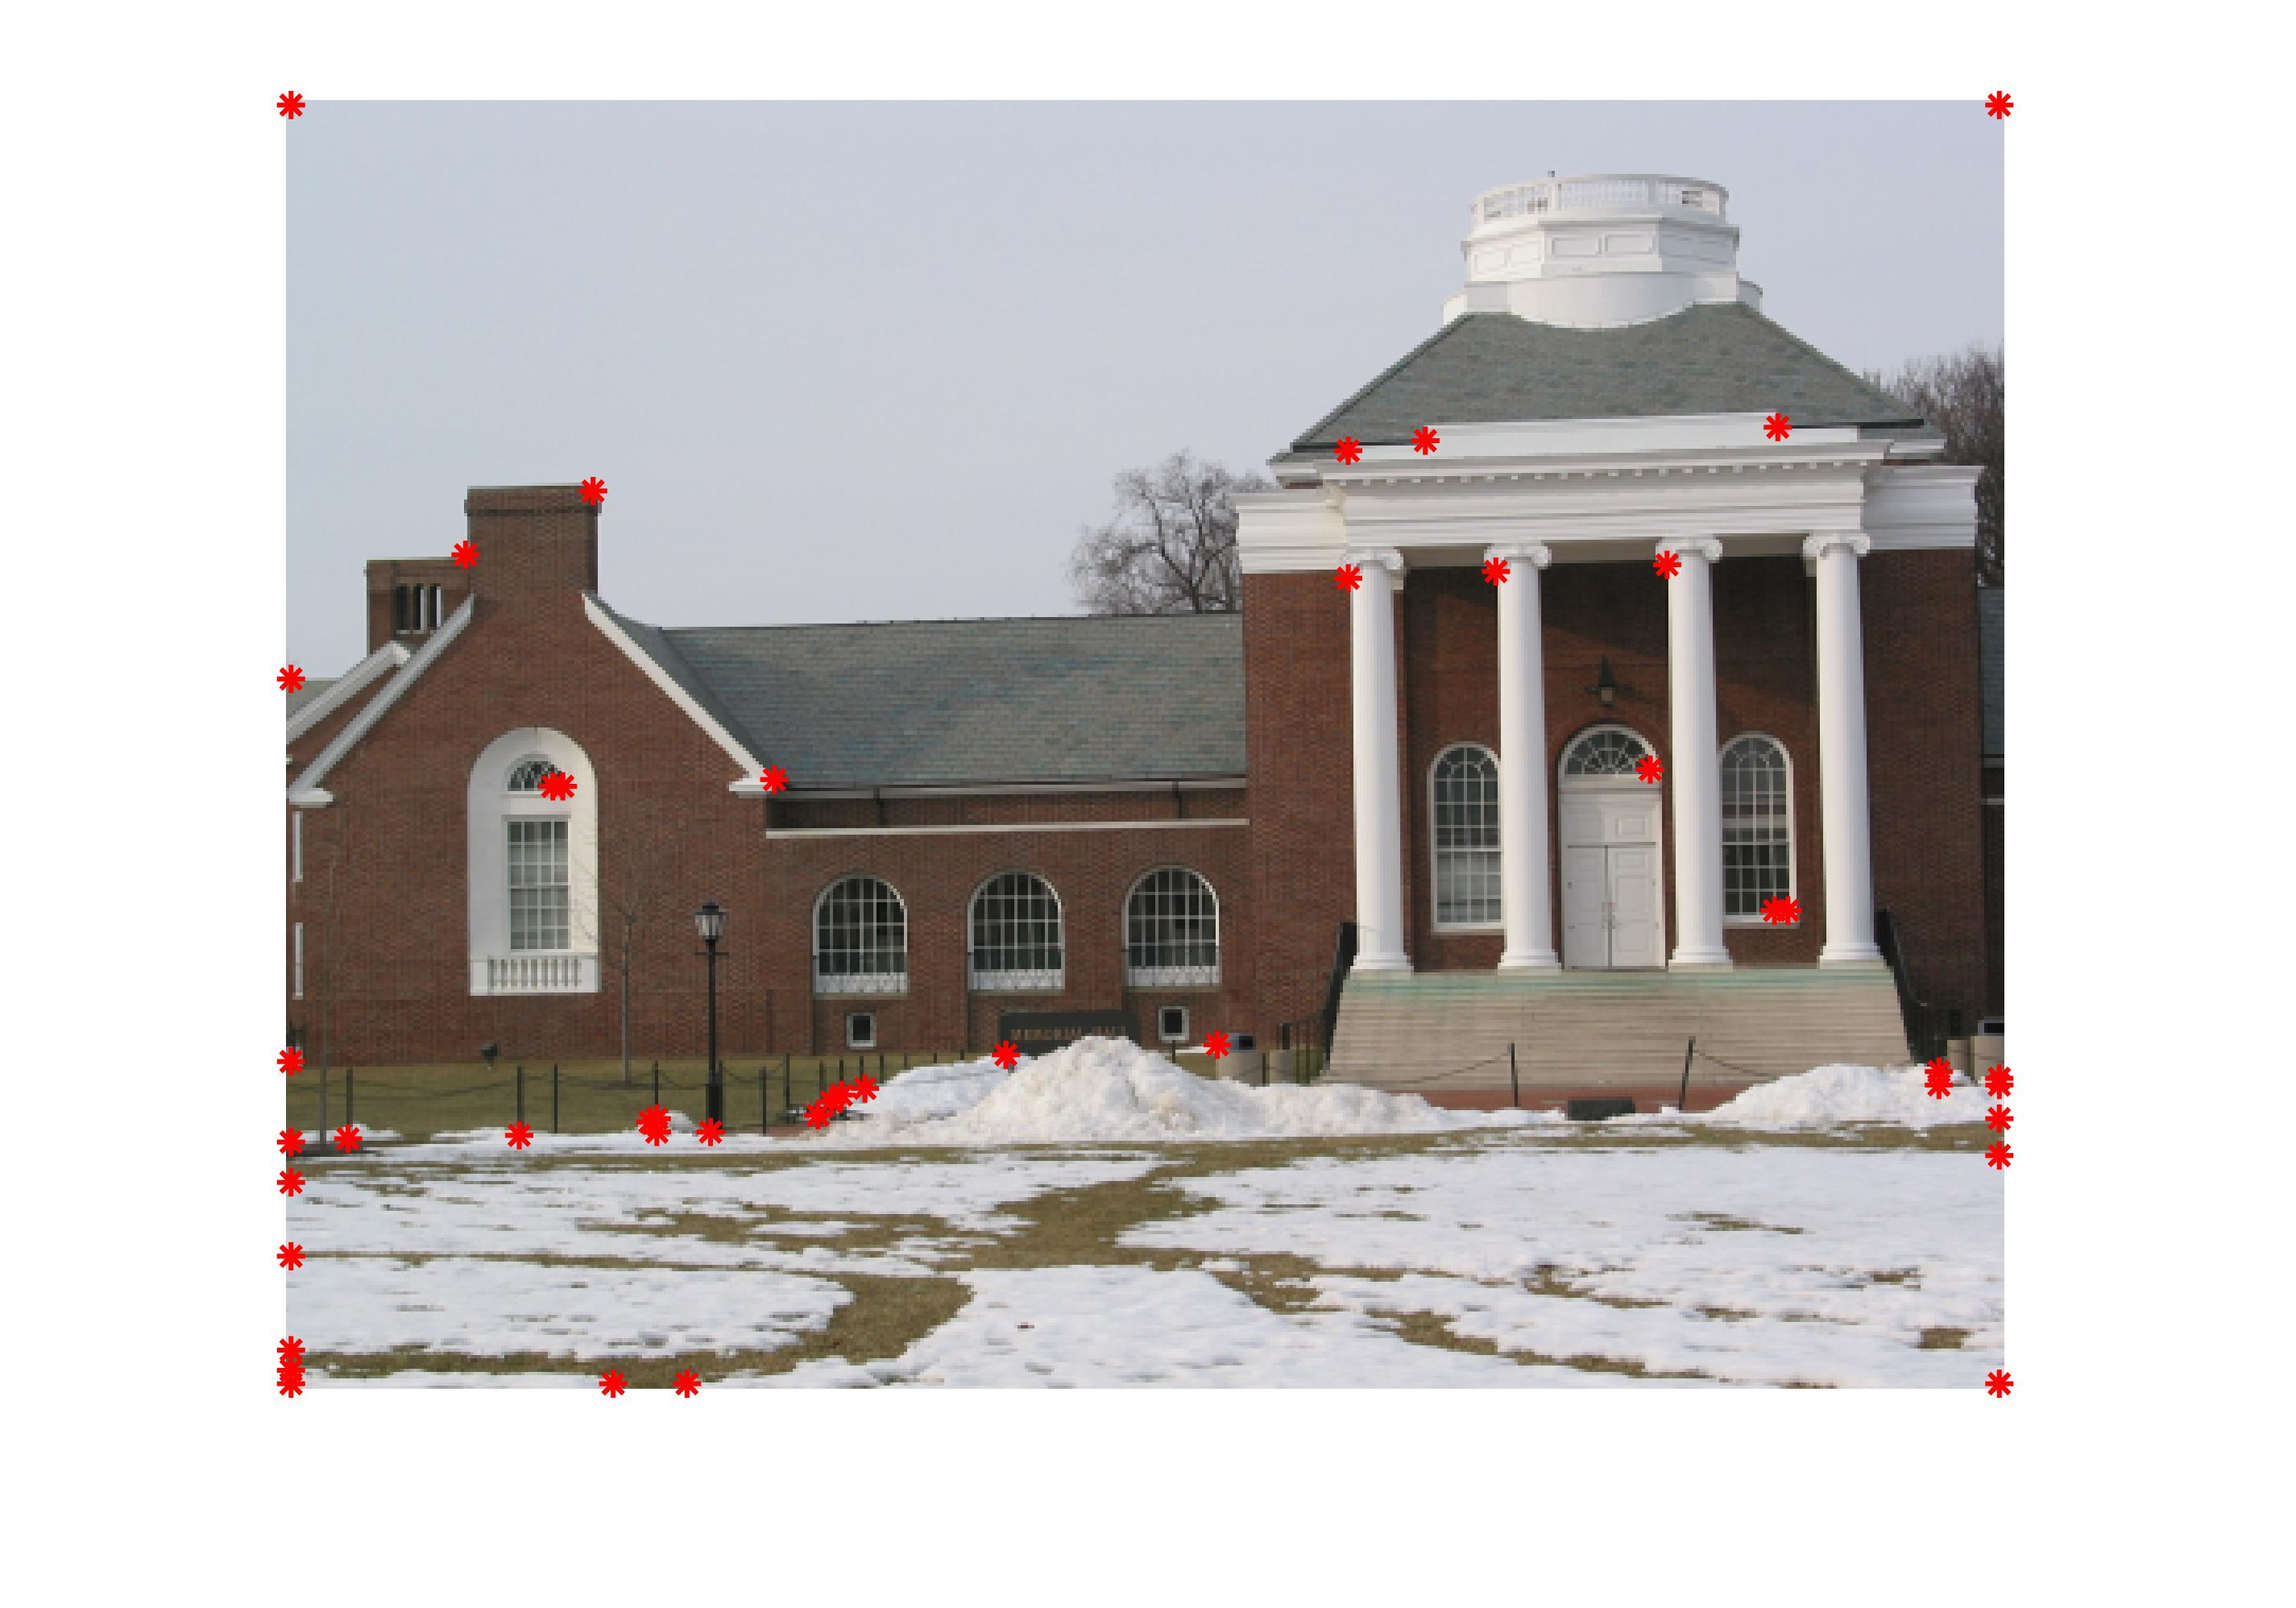
\includegraphics[width=0.45\columnwidth]{HW4_q1_a_I1.jpeg}
}
\subfigure[Result for I3.png] { \label{q1_a_fig:b}
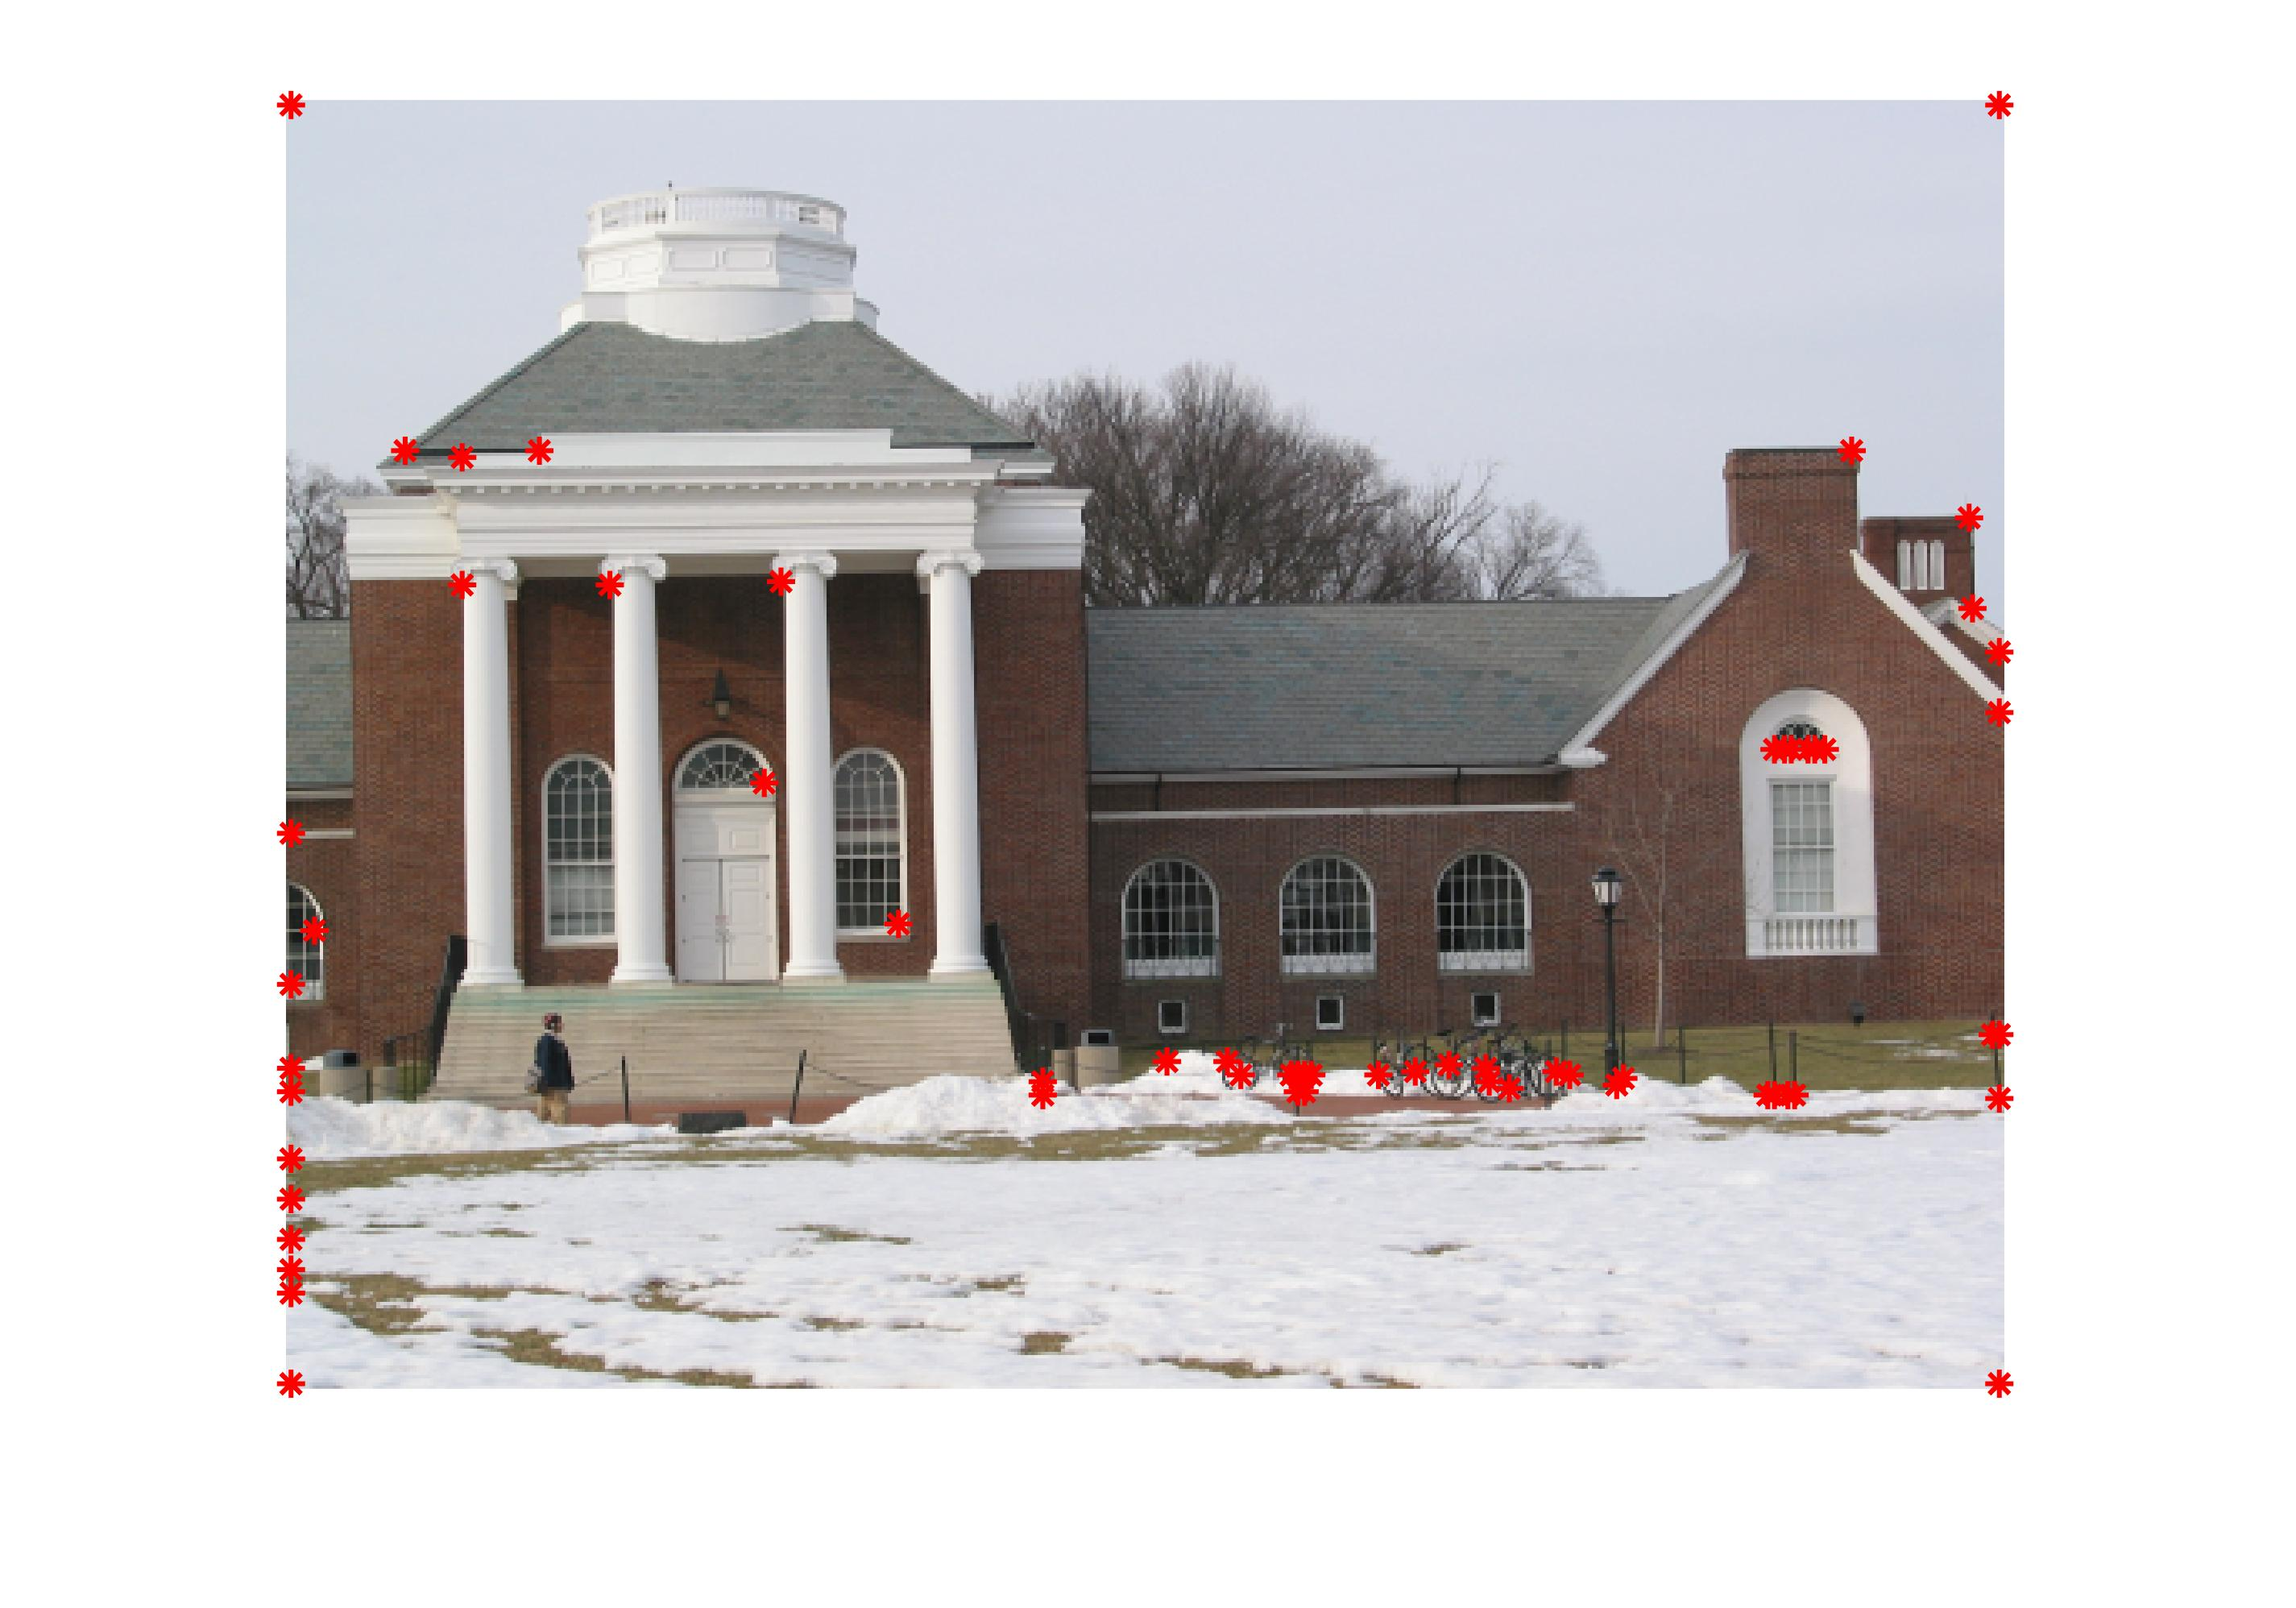
\includegraphics[width=0.45\columnwidth]{HW4_q1_a_I3.jpeg}
}
\caption{Harris Corner Detection, $w=3$}
\label{q1_a_w_3}
\end{figure}

Key steps of the algorithm:\\
Step1, Compute magnitude of the x and y gradients at each pixel.\\
Step2, Due to Harris, construct a Gaussian window M around each pixel.\\
Step3, Compute $\lambda_s$ of second moment matrix $M$ \\
Step4, Compute $R=det(M)-k(tr(M))^2$ \\
Step5, Set proper threshold $T$ \\
Step6, If $R> T$, a corner is detected; then, retain point of local maxima. \\
Step7, Superpose corners on images.\\

More explanation is written in the attach code.\\
\begin{lstlisting}
%% EECS 442 - HW 04 - Q1 Harris Corner Detection
%  ------------------------------------------------------------------------
%  Date: 11 / 21 / 2016
%  Author: Fan Bu
%  ------------------------------------------------------------------------
%  ellipse(ra,rb,ang,x0,y0,C,Nb)
%  ------------------------------------------------------------------------
%  Instructions(Latex code)
% Key steps of the algorithm:\\
% Step1, Compute magnitude of the x and y gradients at each pixel.\\
% Step2, Due to Harris, construct a Gaussian window M around each pixel.\\
% Step3, Compute $\lambda_s$ of second moment matrix $M$ \\
% Step4, Compute $R=det(M)-k(tr(M))^2$ \\
% Step5, Set proper threshold $T$ \\
% Step6, If $R> T$, a corner is detected; then, retain point of local maxima. \\
% Step7, Superpose corners on images.\\

%% ----------------------- Initialization -----------------------
clear all;
close all;
clc;
%% ----------------------- Load data ----------------------------
img1 = imread('I1.png');
img2 = imread('I3.png');

img = img2;
w = 3; %choose window size

%% ------------ Compute M,R and ellipse parameter --------
% translate to gray image
gray_img = rgb2gray(img);
[height,width] = size(gray_img);
% initialize corner position
is_edge = zeros(height, width);
% initialize R score
R = zeros(height, width);

% applying sobel edge detector in the horizontal direction
fx = [-1 0 1;
    -1 0 1;
    -1 0 1];
Ix = filter2(fx,gray_img);
% applying sobel edge detector in the vertical direction
fy = [1 1 1;
    0 0 0;
    -1 -1 -1];
Iy = filter2(fy,gray_img);
% compute terms for second moment matrix M
Ix2 = Ix.^2;
Iy2 = Iy.^2;
Ixy = Ix.*Iy;

% perform gaussian filtering for eliminating noises
h= fspecial('gaussian',[w w],2);
Ix2 = filter2(h,Ix2);
Iy2 = filter2(h,Iy2);
Ixy = filter2(h,Ixy);

% Initialize Perem
Rmax = 0;
figure;
imshow(img);
hold on;
for i = 1:height
    for j = 1:width
        % compute second moment matrix M
        M = [
            Ix2(i,j), Ixy(i,j);
            Ixy(i,j) Iy2(i,j)
            ];
        % compute R(i,j) = det(M)-0.04*(trace(M))^2
        R(i,j) = det(M)-0.04*(trace(M))^2;
        if R(i,j) > Rmax
           Rmax = R(i,j);
        end;

    end;
end;
num_edge = 0;
Rmax
T=0.1*Rmax
% determine corner by comparing with threshold and all neighbor points
for i = 2:height-1
    for j = 2:width-1
        if R(i,j) > T ...
            && R(i,j) > R(i-1,j-1) ...
            && R(i,j) > R(i-1,j) ...
            && R(i,j) > R(i-1,j+1) ...
            && R(i,j) > R(i,j-1) ...
            && R(i,j) > R(i,j+1) ...
            && R(i,j) > R(i+1,j-1) ...
            && R(i,j) > R(i+1,j) ...
            && R(i,j) > R(i+1,j+1)

            is_edge(i,j) = 1;
            num_edge = num_edge+1;
        end;
    end;
end;
[edge_col, edge_row] = find(is_edge == 1);
num_edge
%% -------------- Draw corners on image and save -----------------
plot(edge_row, edge_col,'r*','linewidth',1.1);
print(gcf,'-djpeg' ,'HW4_q1_a_I3.jpeg','-r400')
\end{lstlisting}
\subsection*{(b)}
Repeat this step by using different sizes of the window $W = 3, 4, 6, 9$. Results are shown in the following figures (Note that pictures are zoomed in):\\

\begin{figure}[H] \centering
\subfigure[Result for I1.png] { \label{q1_b_w_3_fig:a}
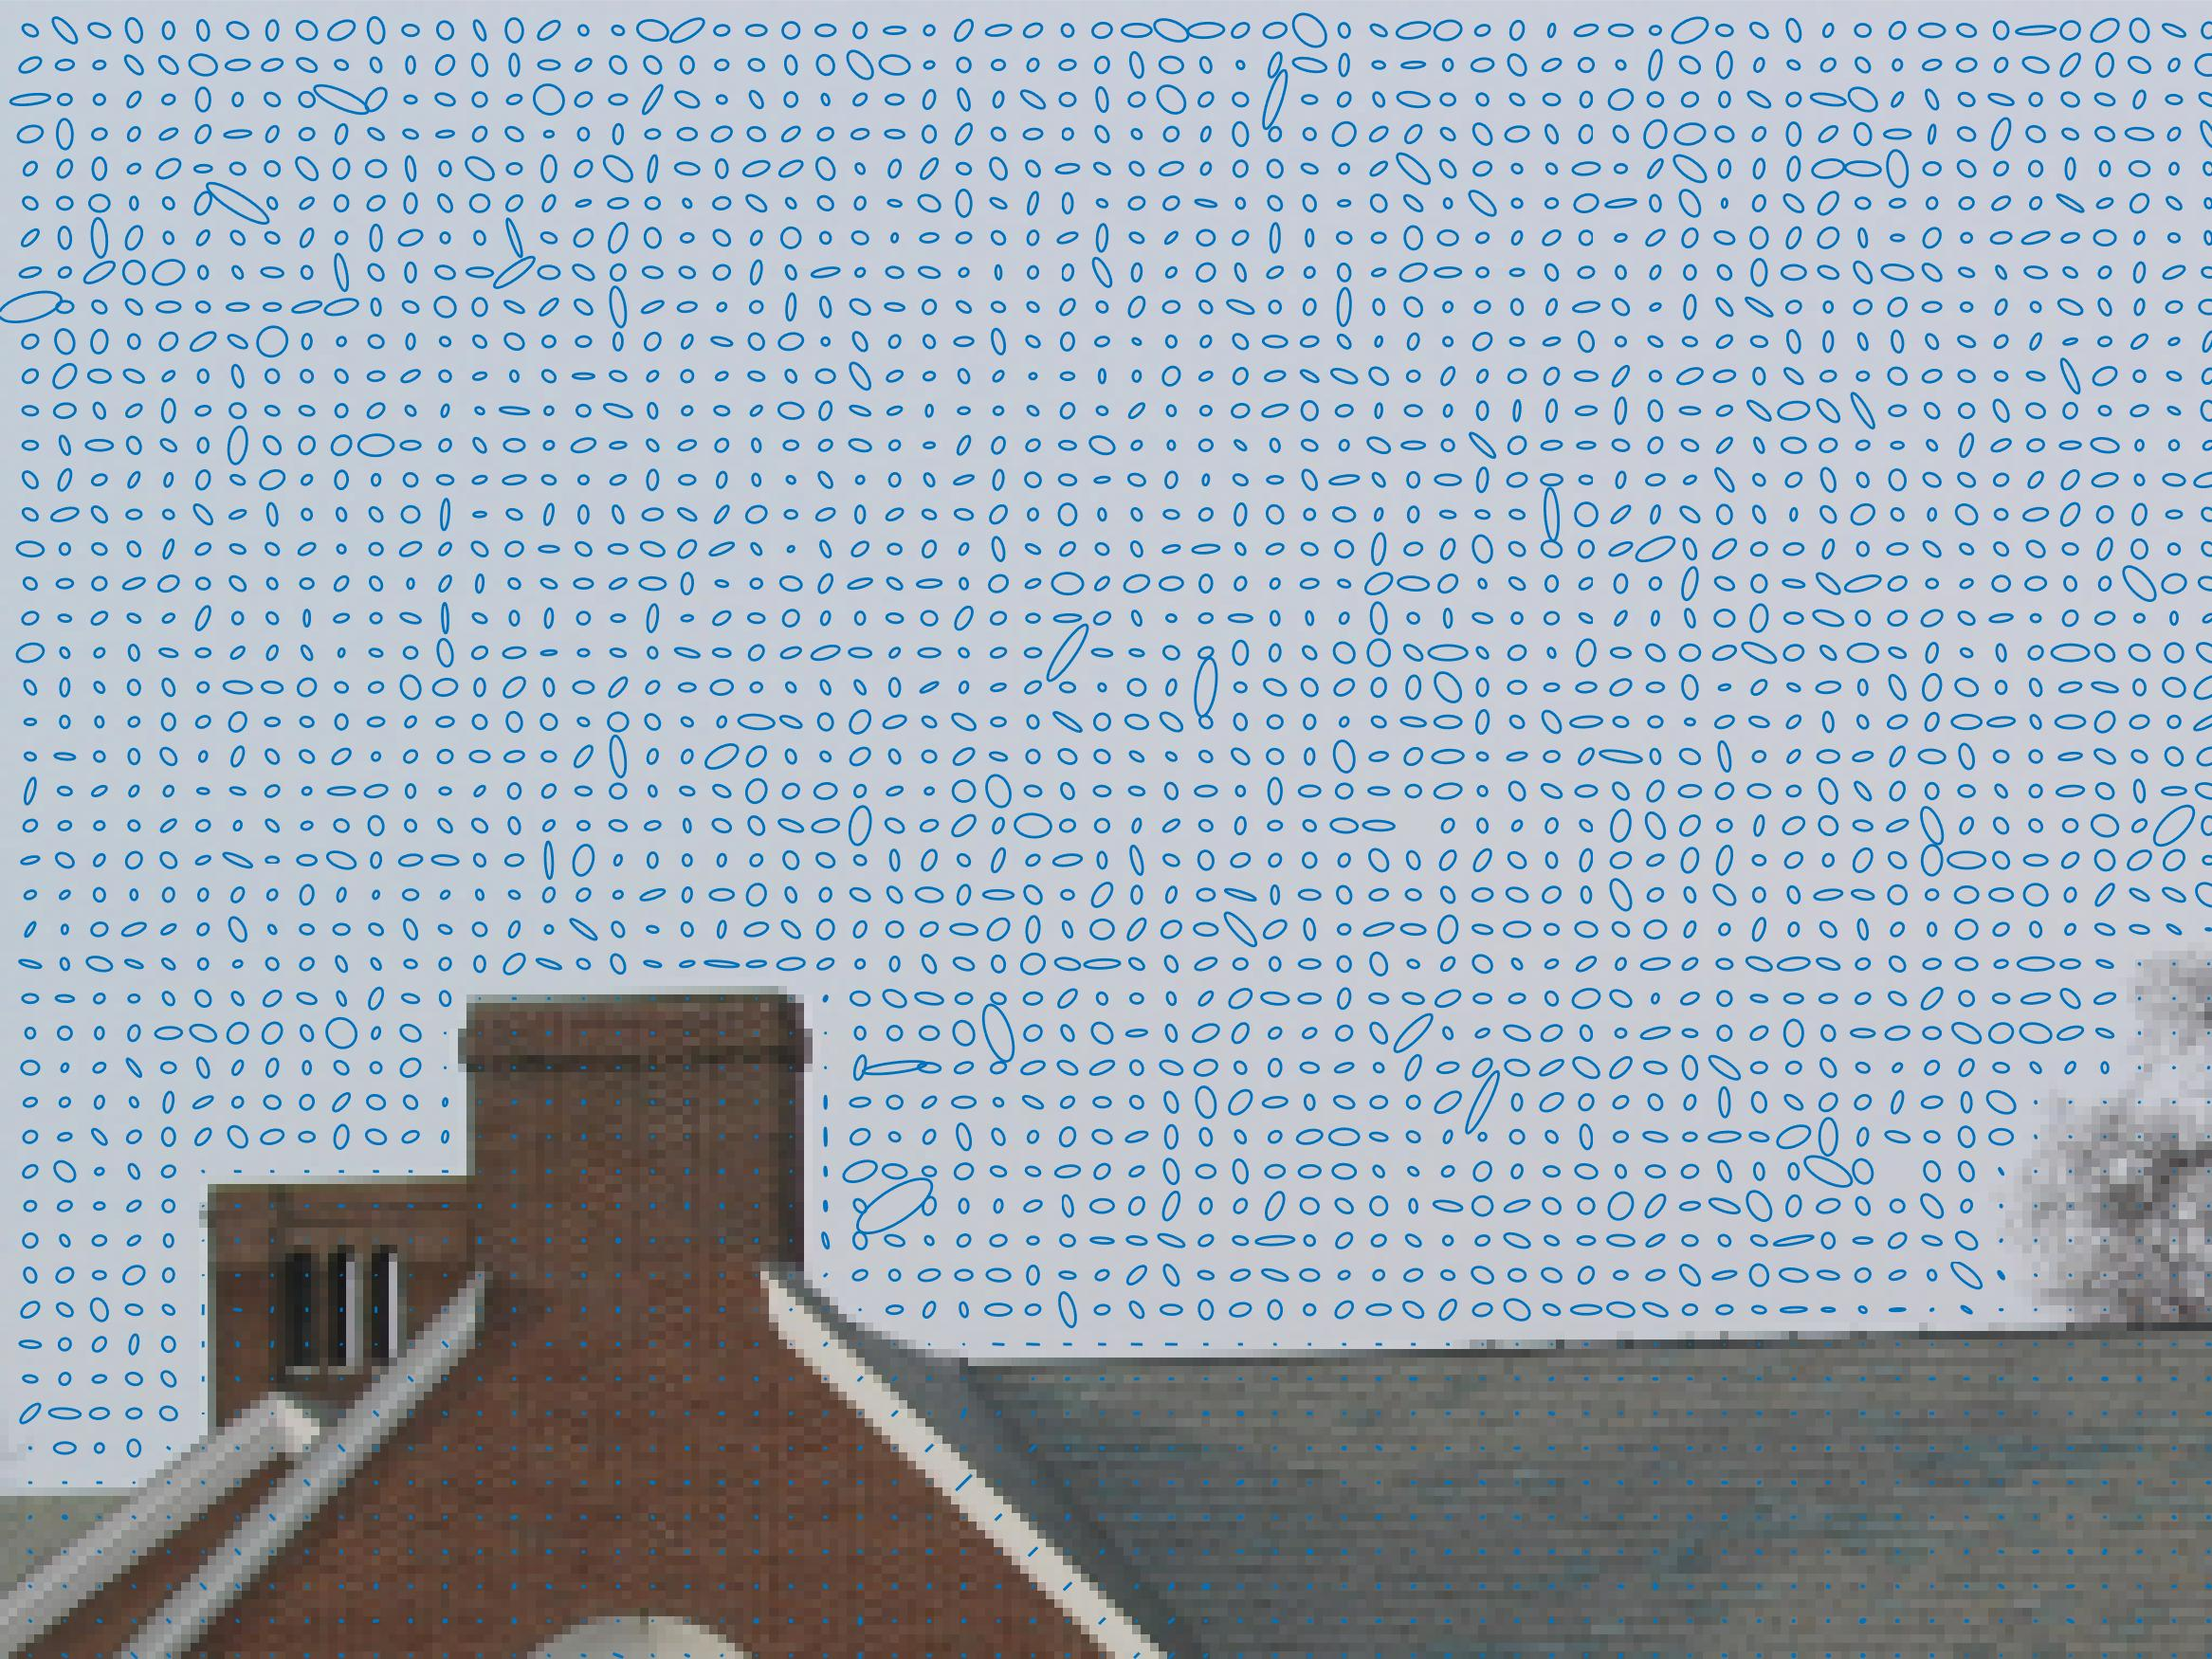
\includegraphics[width=0.9\columnwidth]{HW4_q1_b_w_3_I1.jpeg}
}
\subfigure[Result for I3.png] { \label{q1_b_w_3_fig:b}
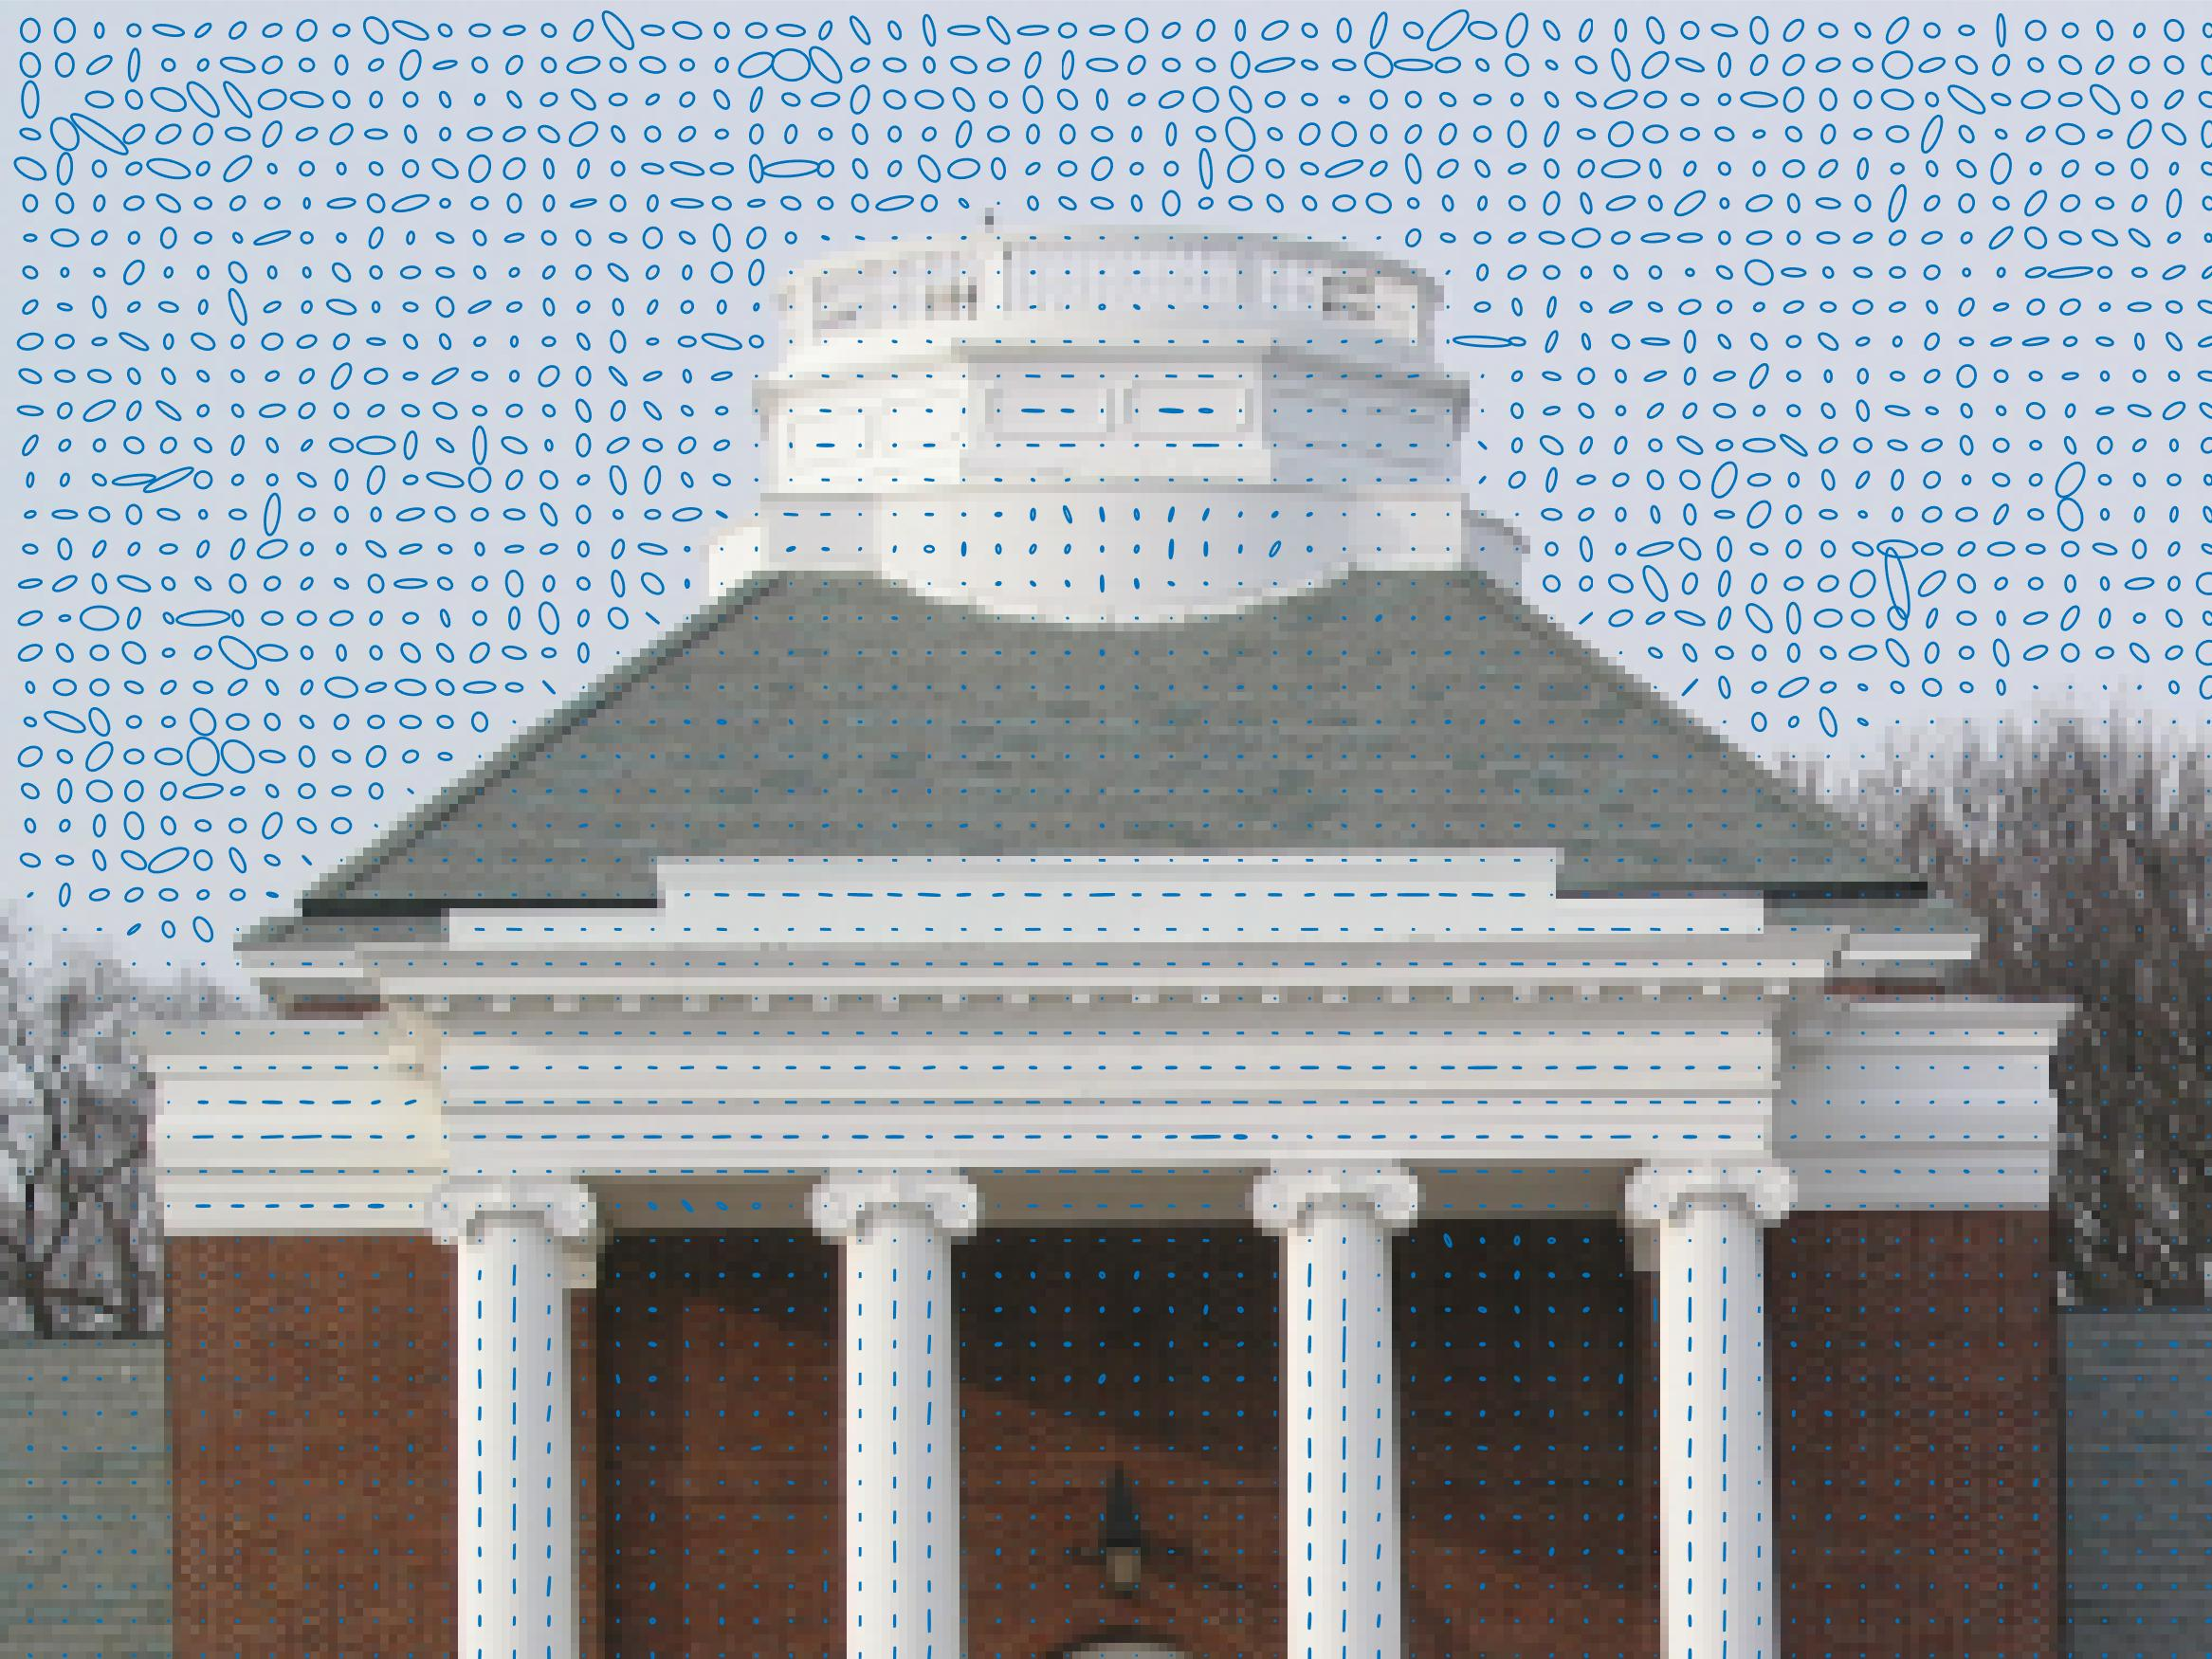
\includegraphics[width=0.9\columnwidth]{HW4_q1_b_w_3_I3.jpeg}
}
\caption{Superimpose Ellipses, $w=3$}
\label{q1_b_w_3}
\end{figure}

\begin{figure}[H] \centering
\subfigure[Result for I1.png] { \label{q1_b_w_4_fig:a}
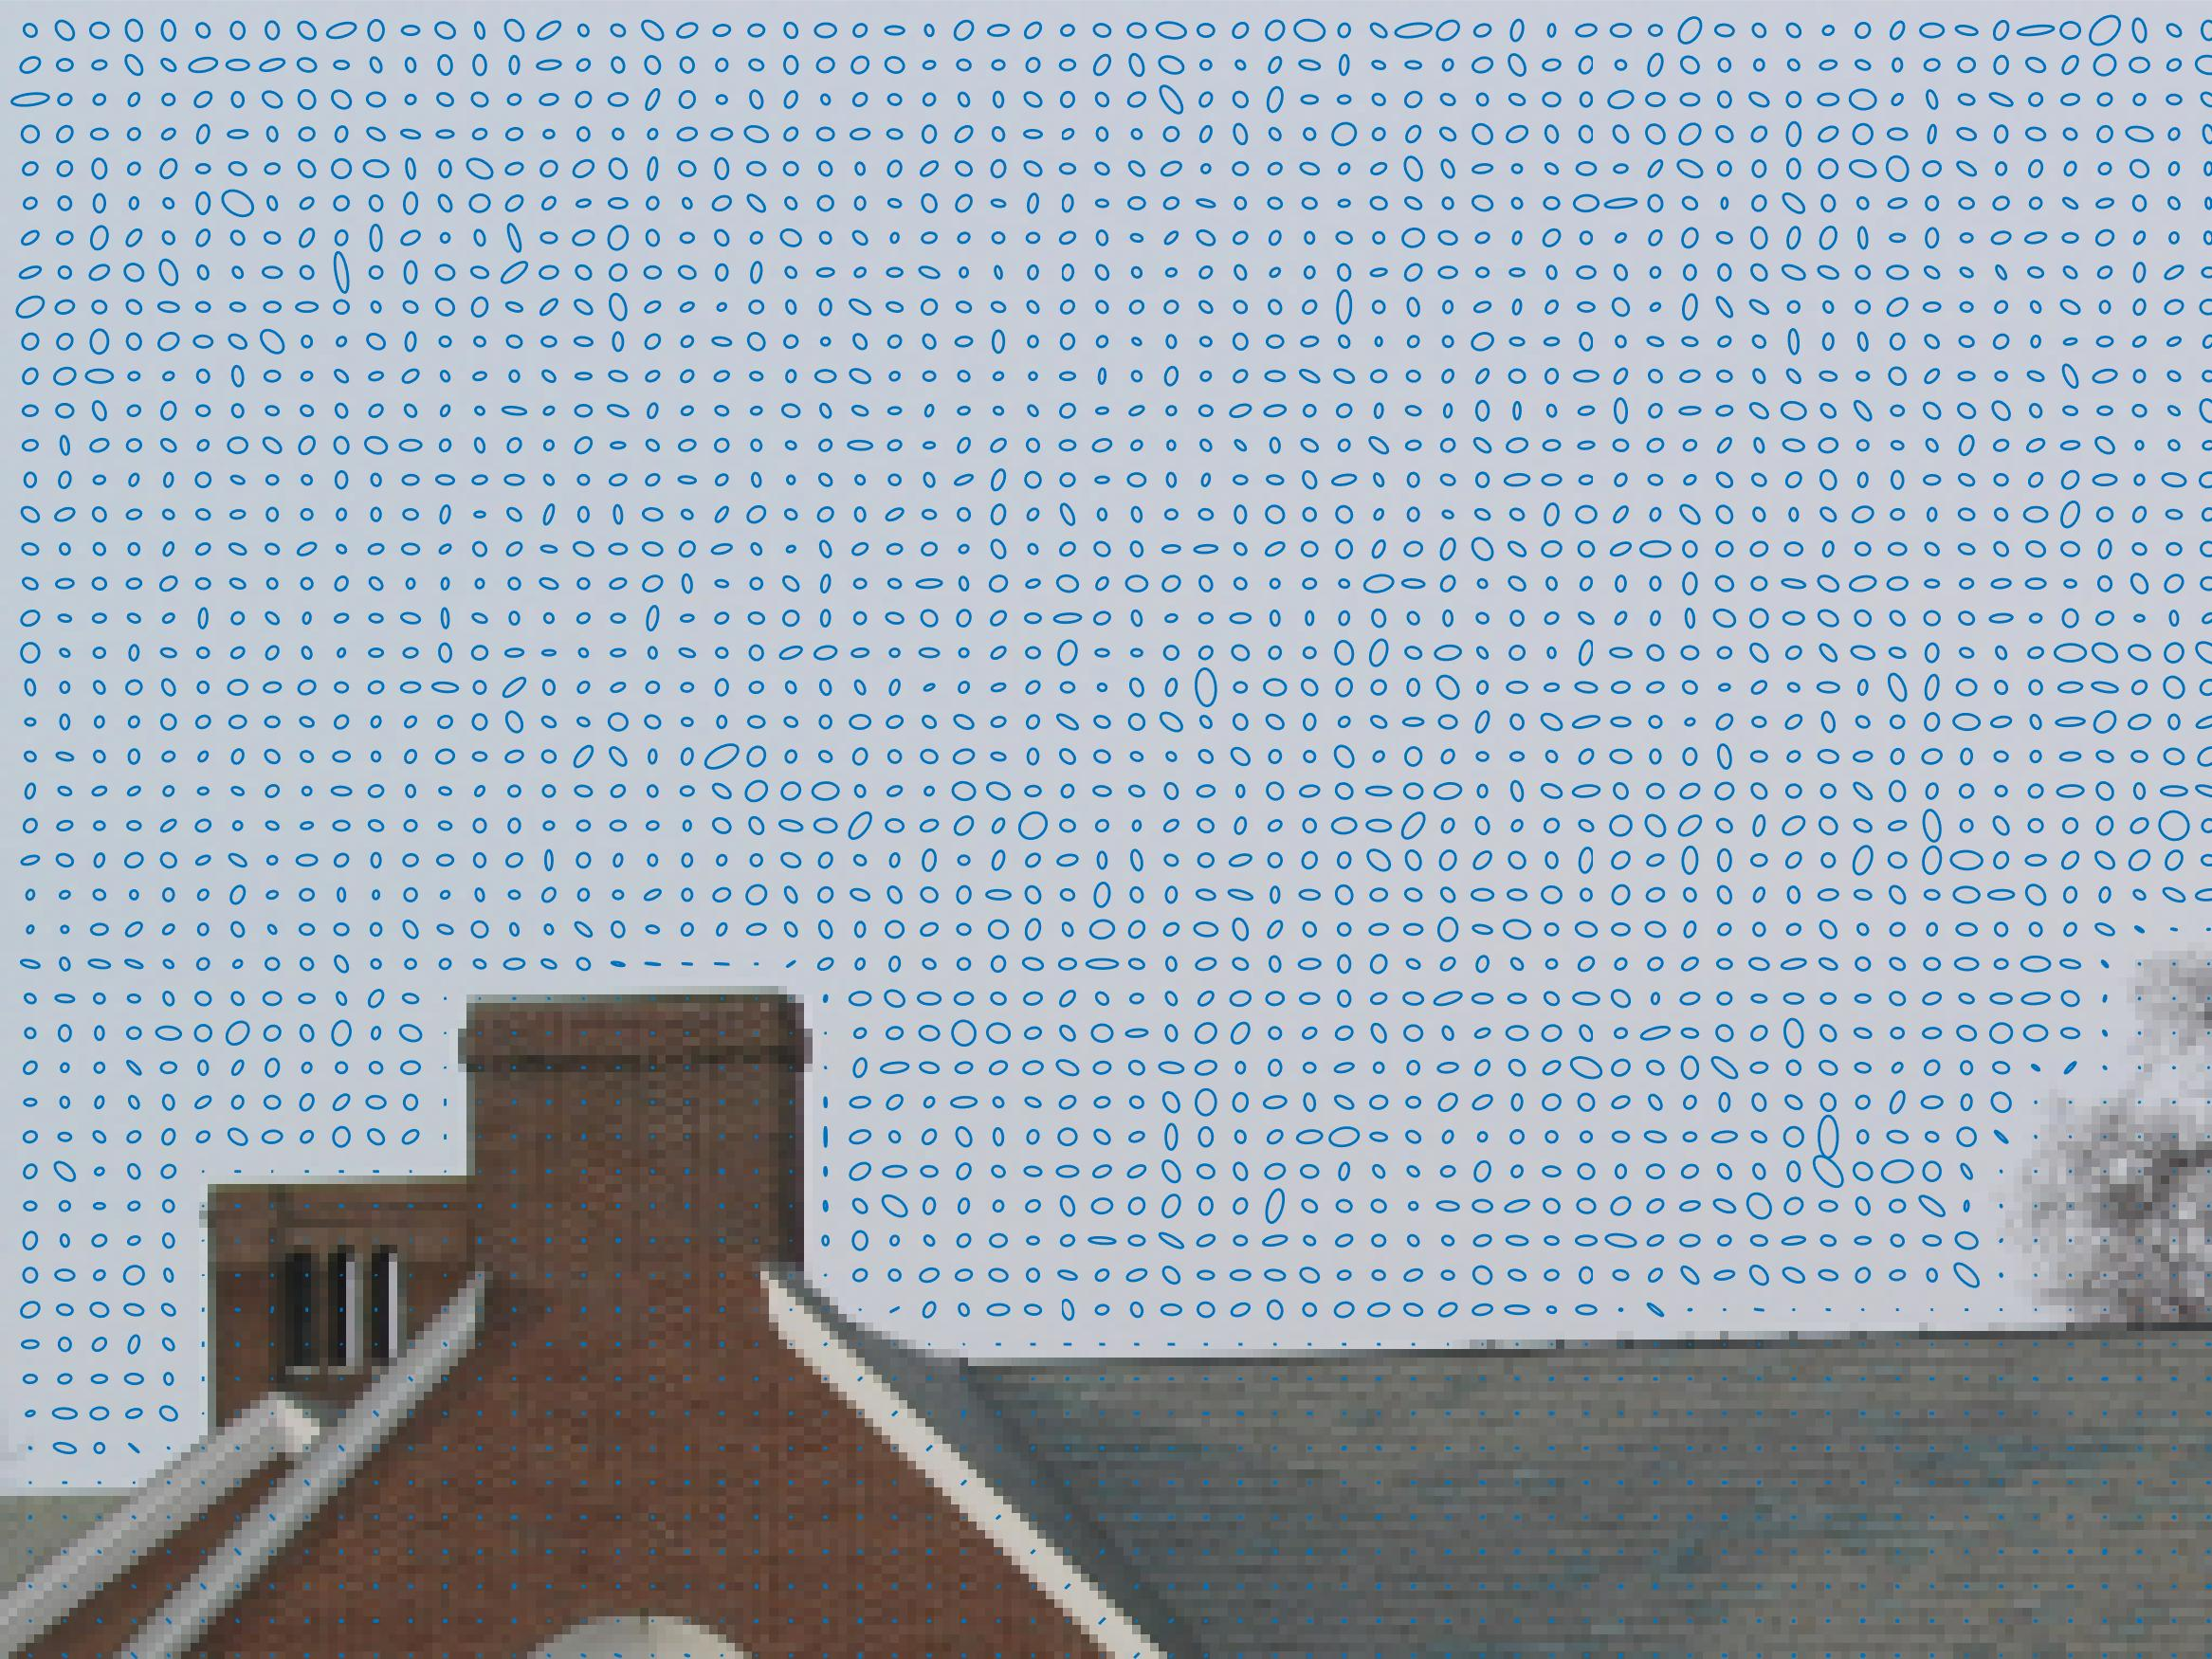
\includegraphics[width=0.9\columnwidth]{HW4_q1_b_w_4_I1.jpeg}
}
\subfigure[Result for I3.png] { \label{q1_b_w_4_fig:b}
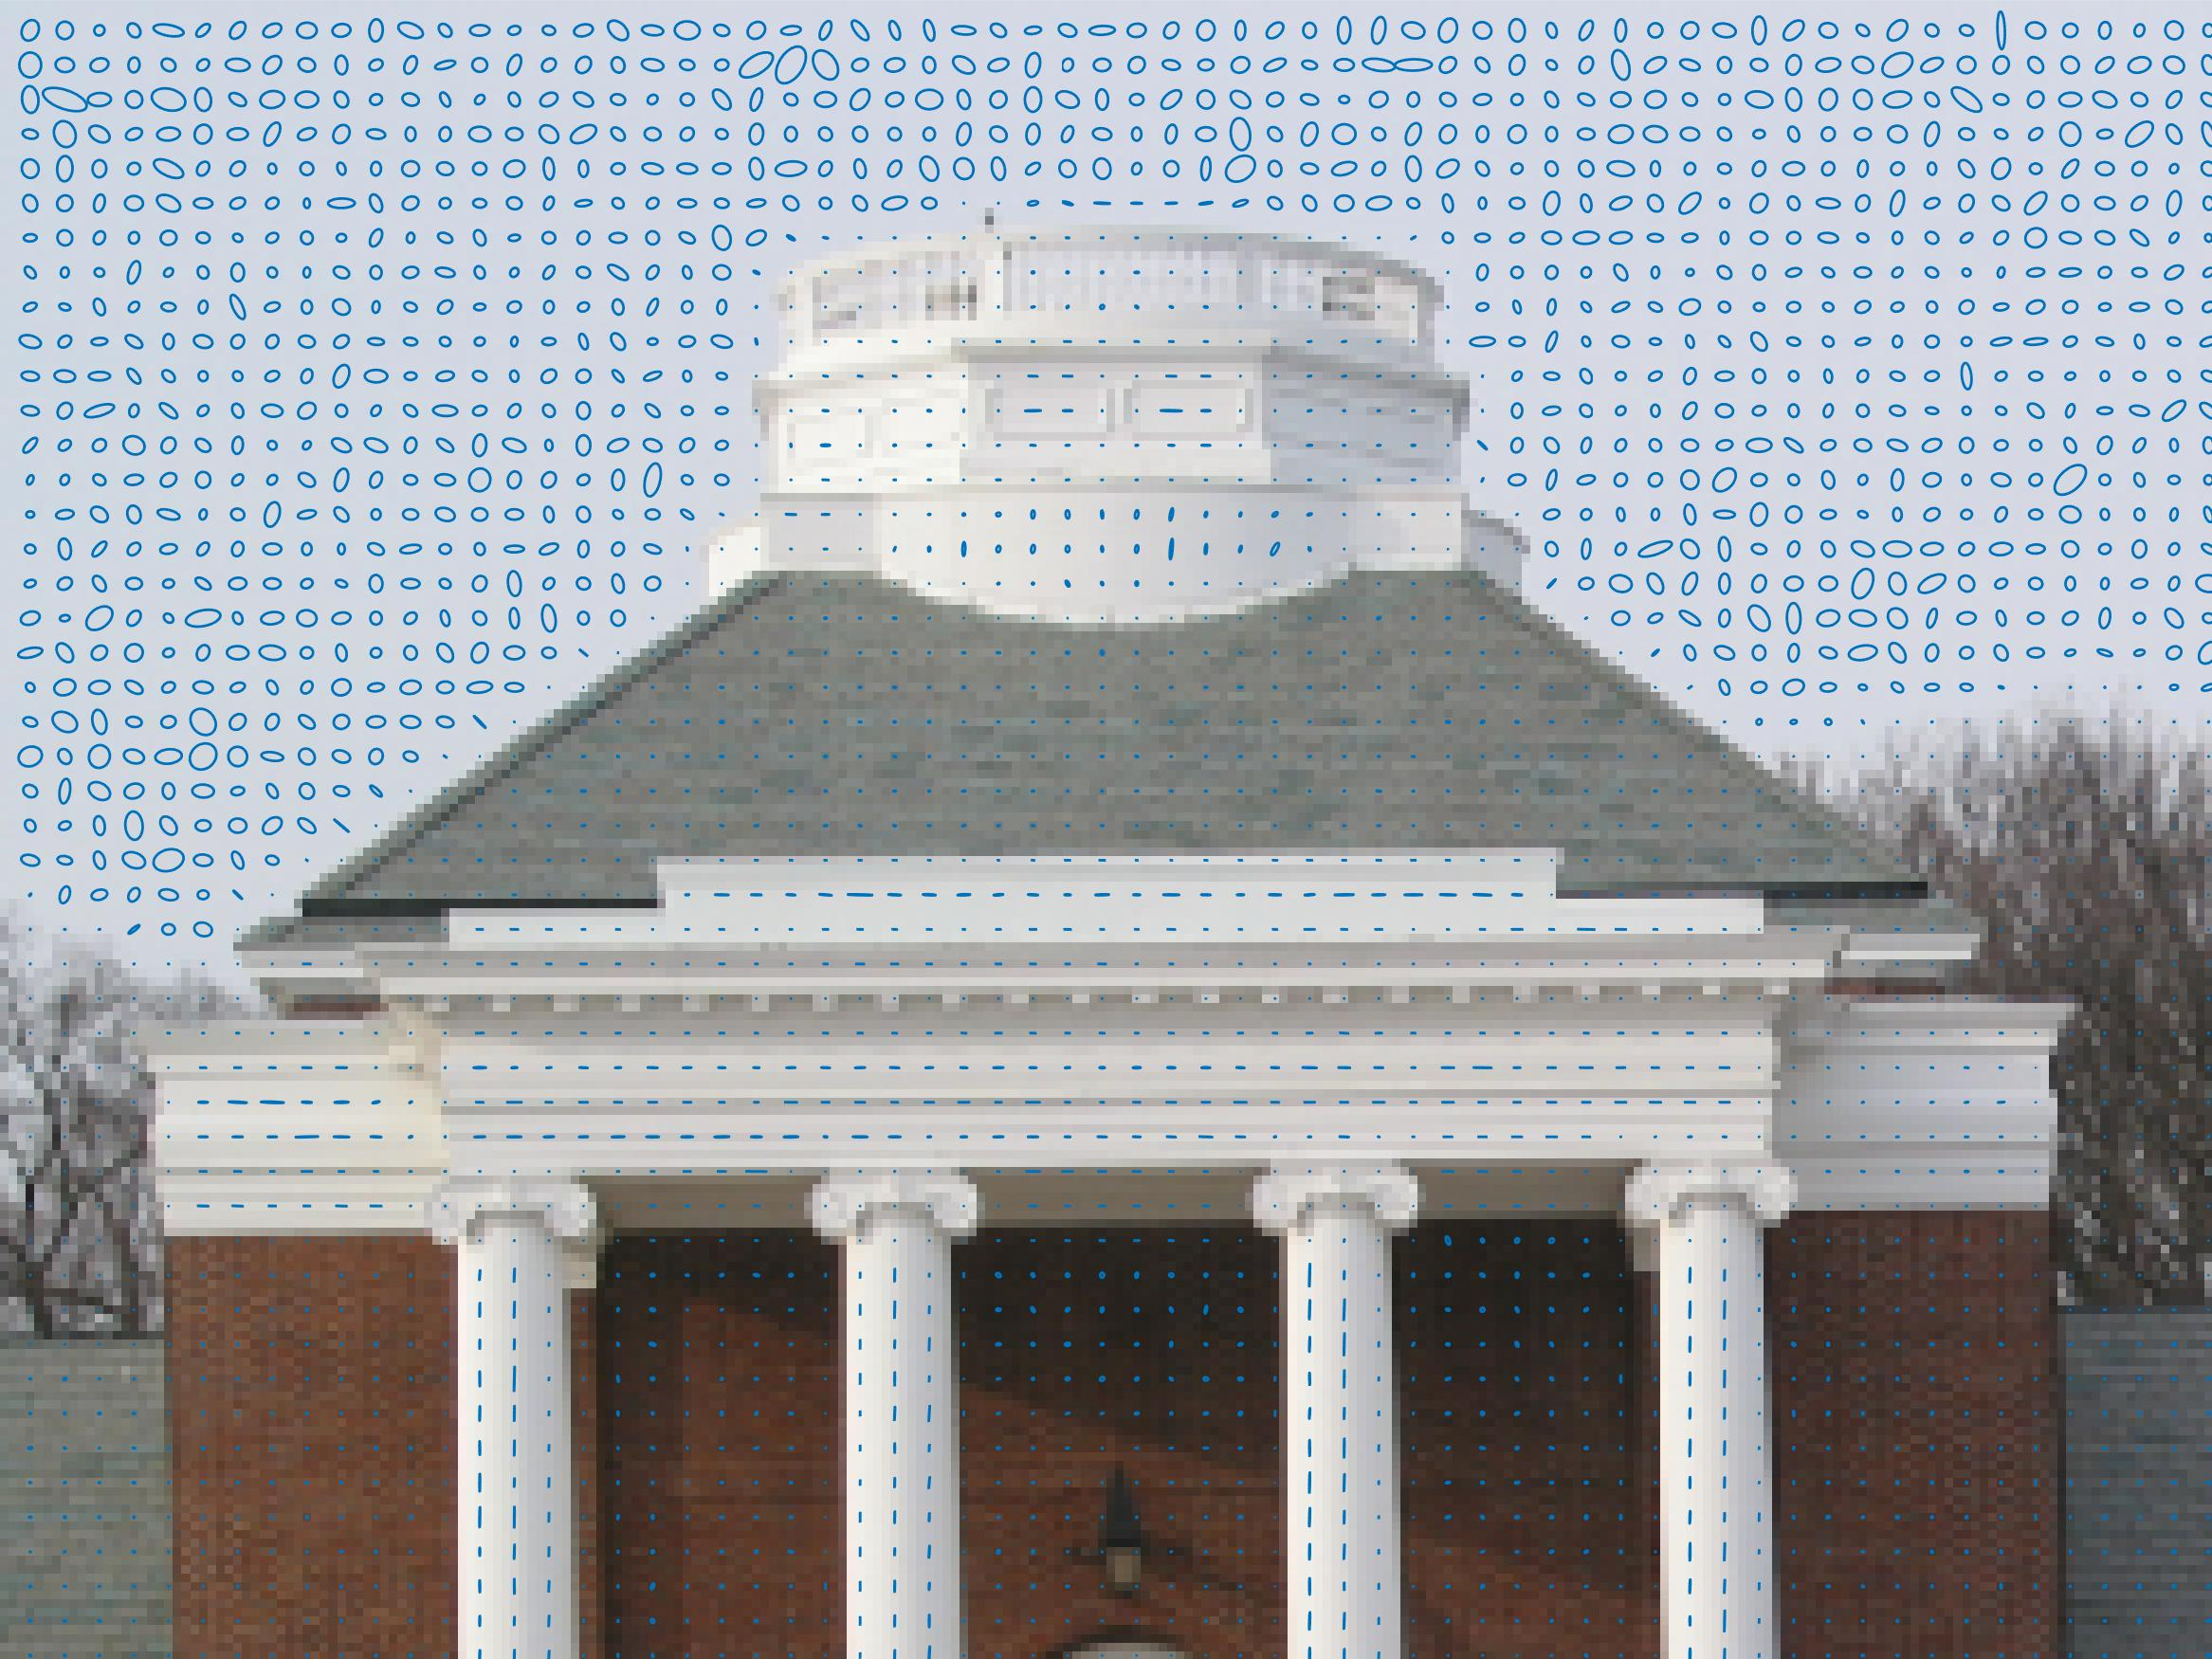
\includegraphics[width=0.9\columnwidth]{HW4_q1_b_w_4_I3.jpeg}
}
\caption{Superimpose Ellipses, $w=4$}
\label{q1_b_w_4}
\end{figure}

\begin{figure}[H] \centering
\subfigure[Result for I1.png] { \label{q1_b_w_6_fig:a}
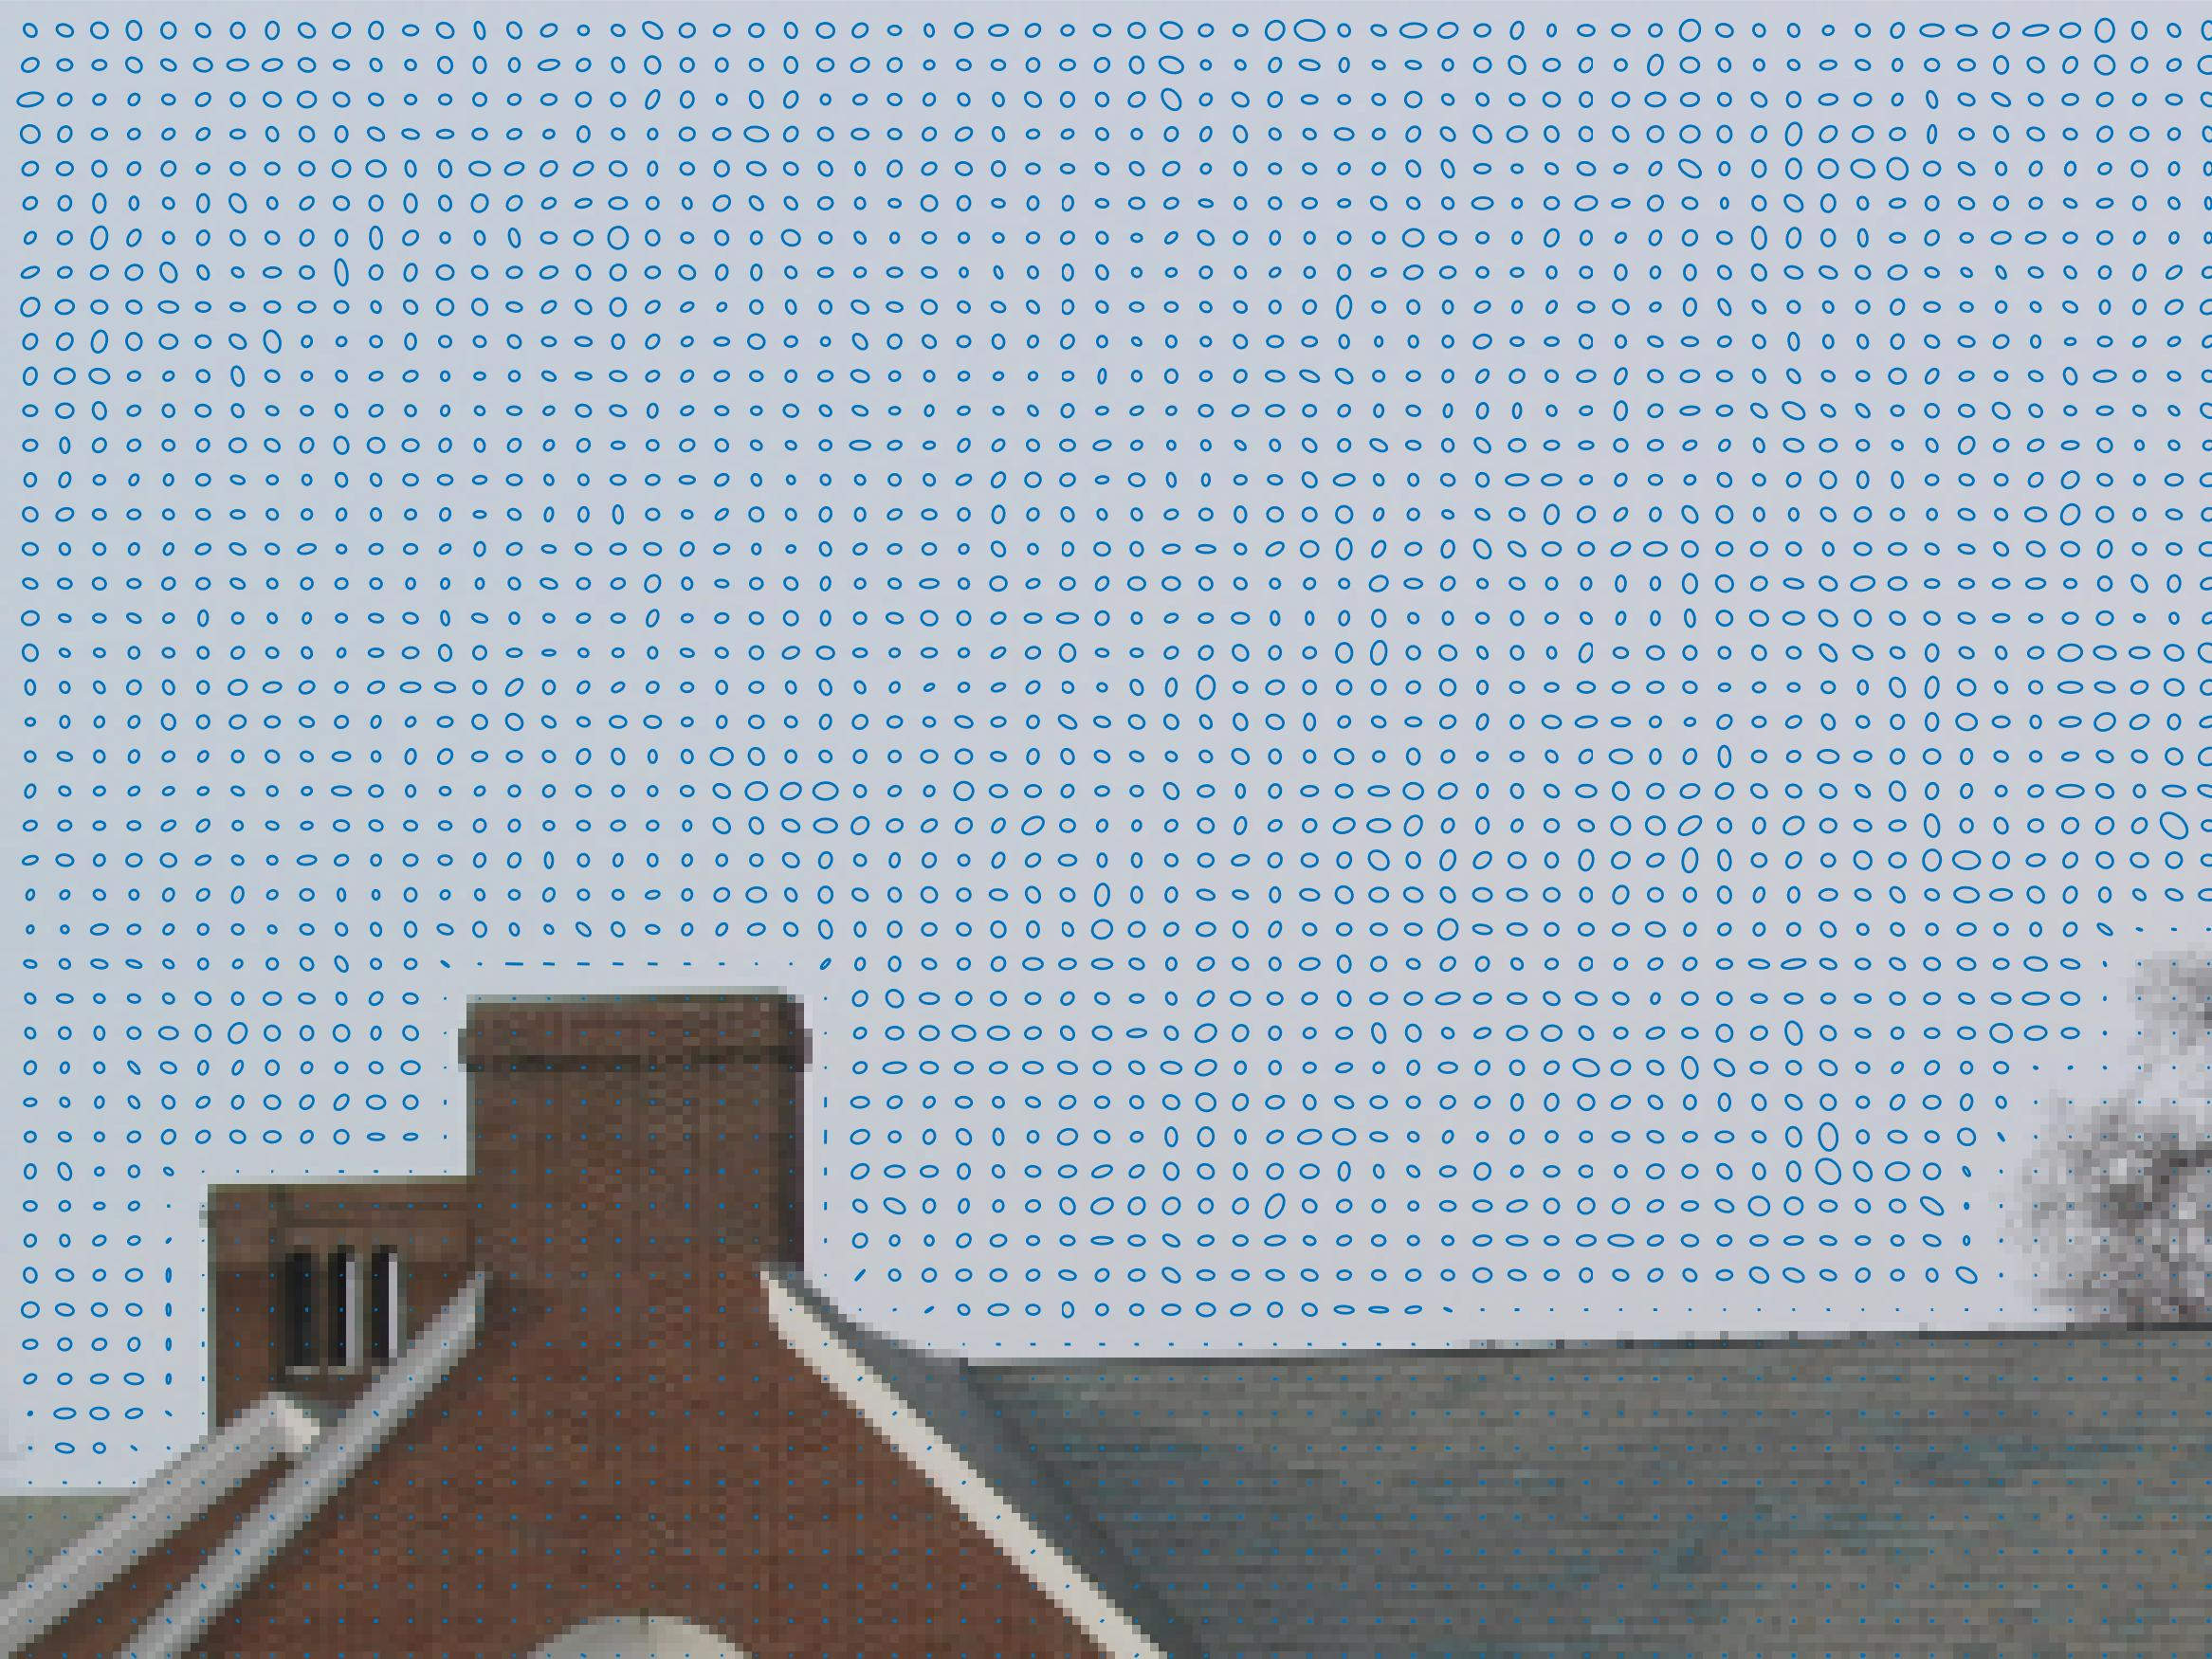
\includegraphics[width=0.9\columnwidth]{HW4_q1_b_w_6_I1.jpeg}
}
\subfigure[Result for I3.png] { \label{q1_b_w_6_fig:b}
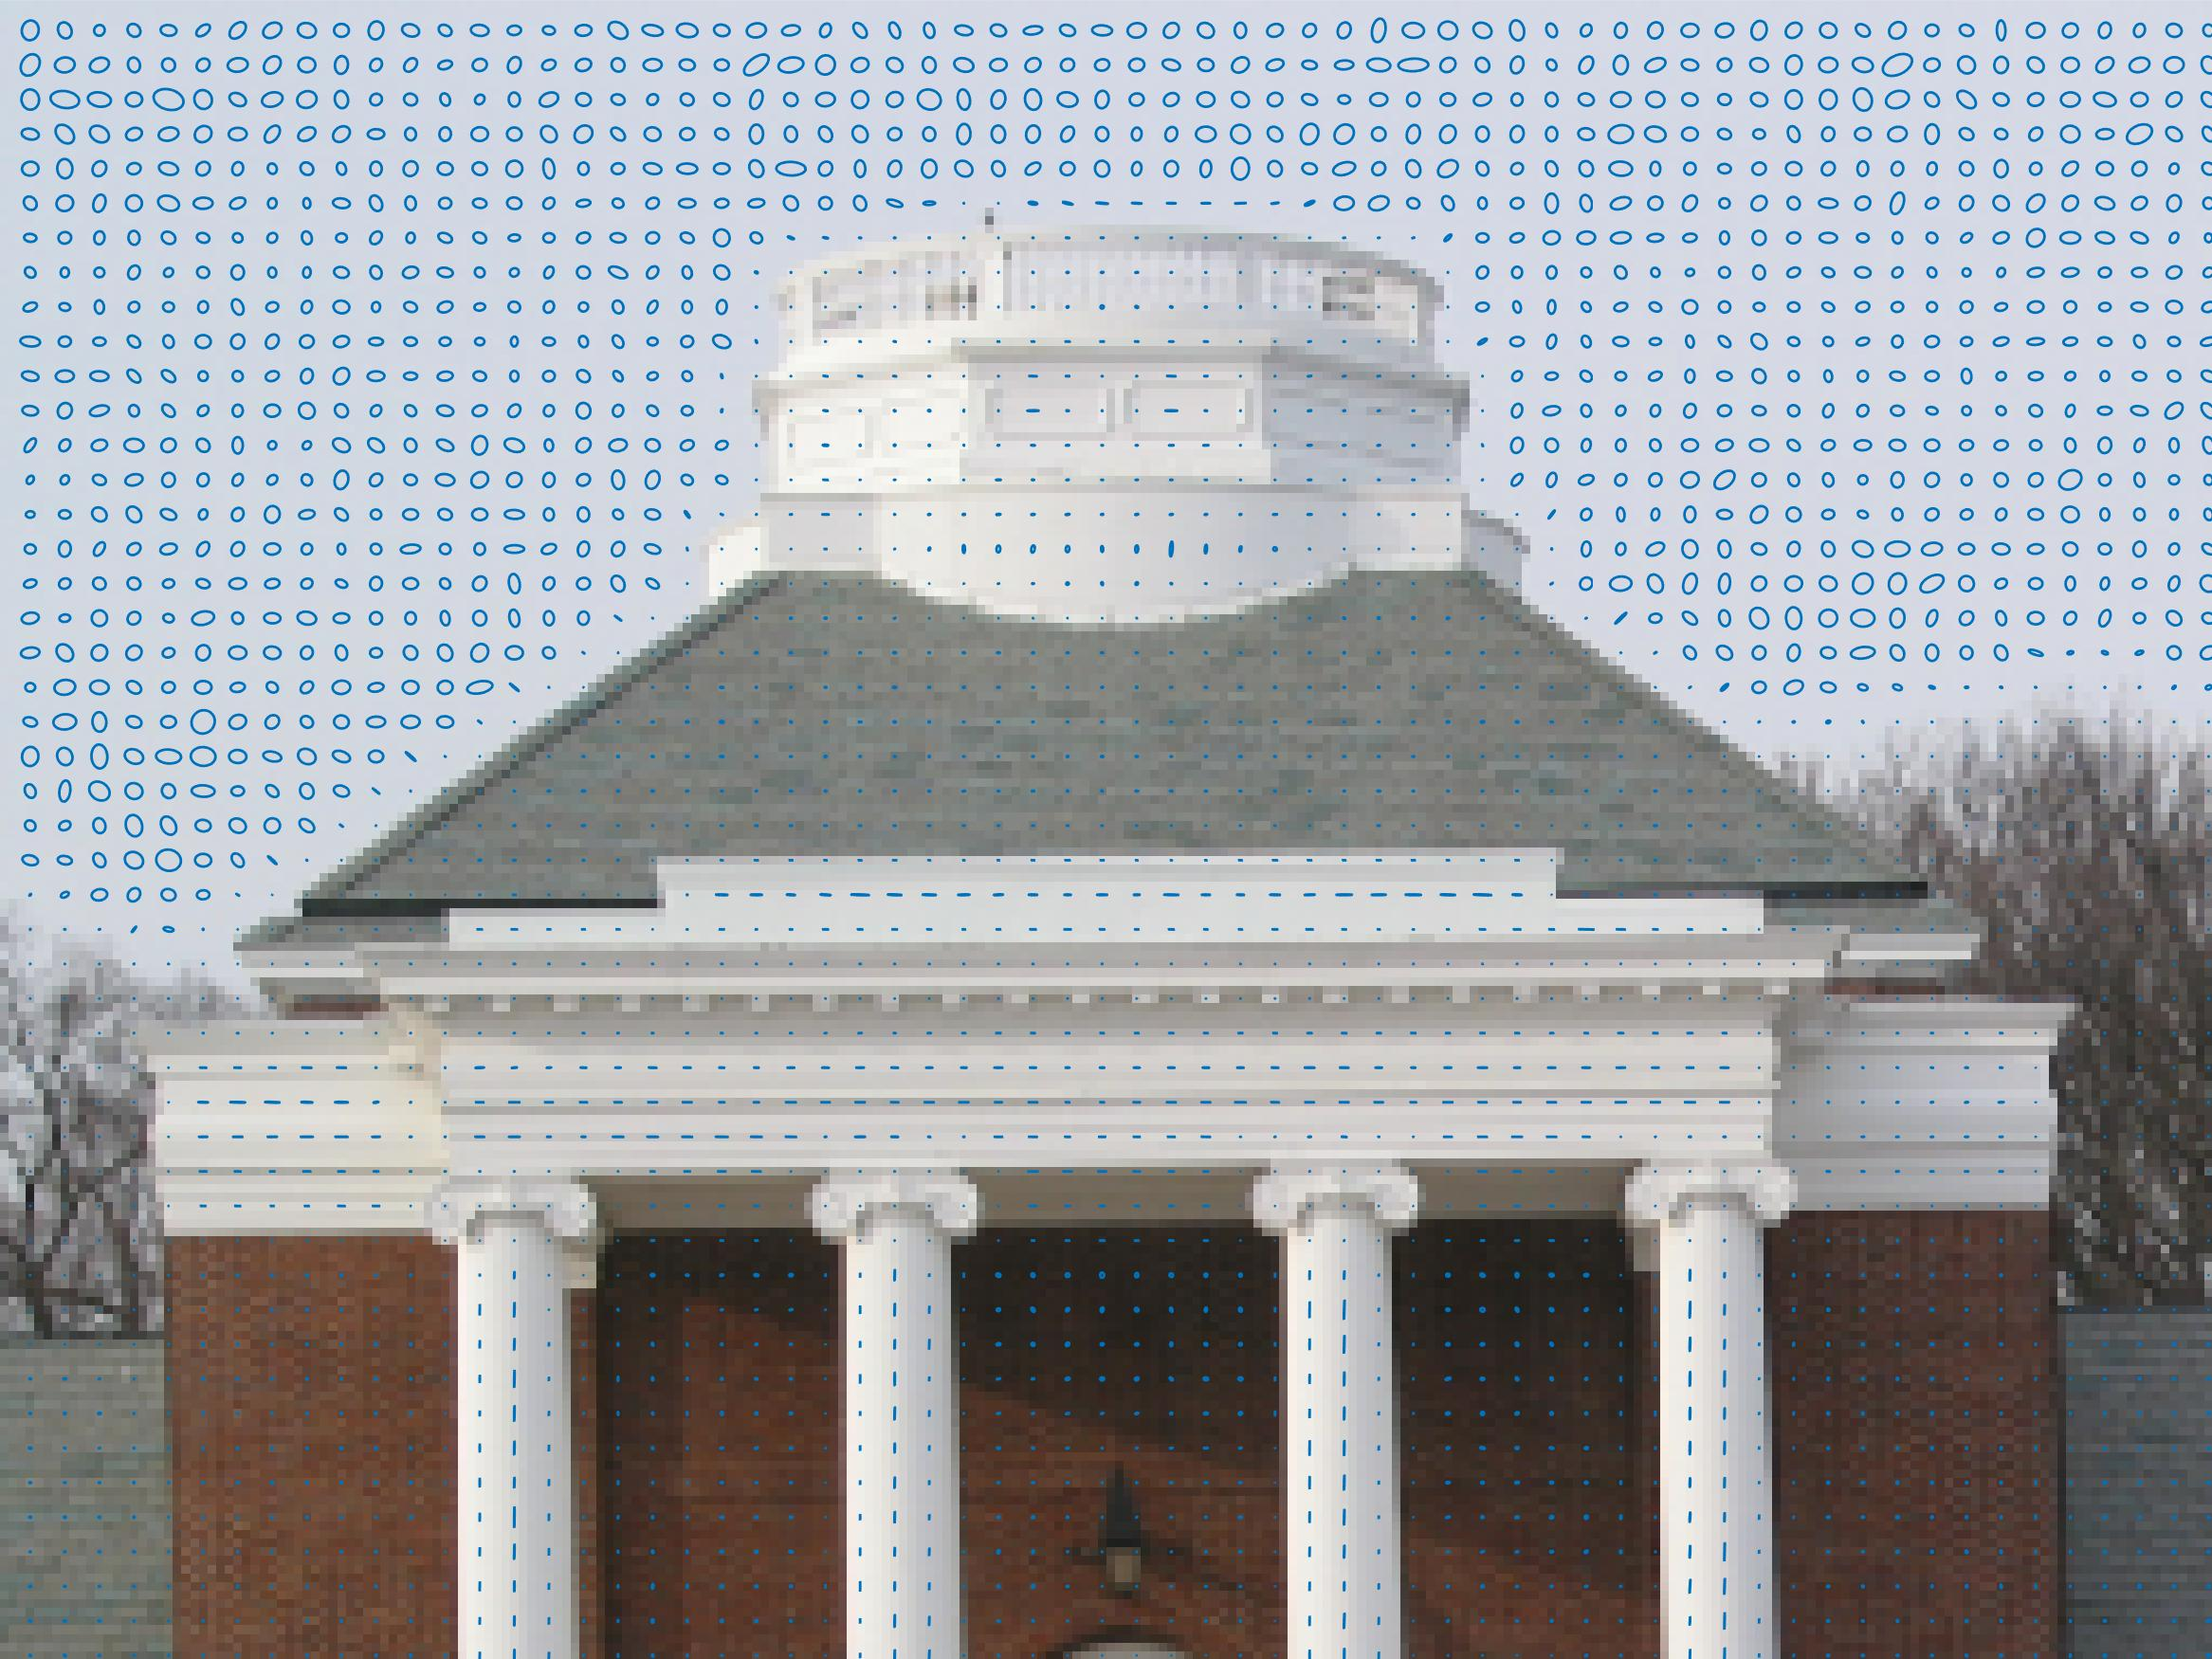
\includegraphics[width=0.9\columnwidth]{HW4_q1_b_w_6_I3.jpeg}
}
\caption{Superimpose Ellipses, $w=6$}
\label{q1_b_w_6}
\end{figure}

\begin{figure}[H] \centering
\subfigure[Result for I1.png] { \label{q1_b_w_9_fig:a}
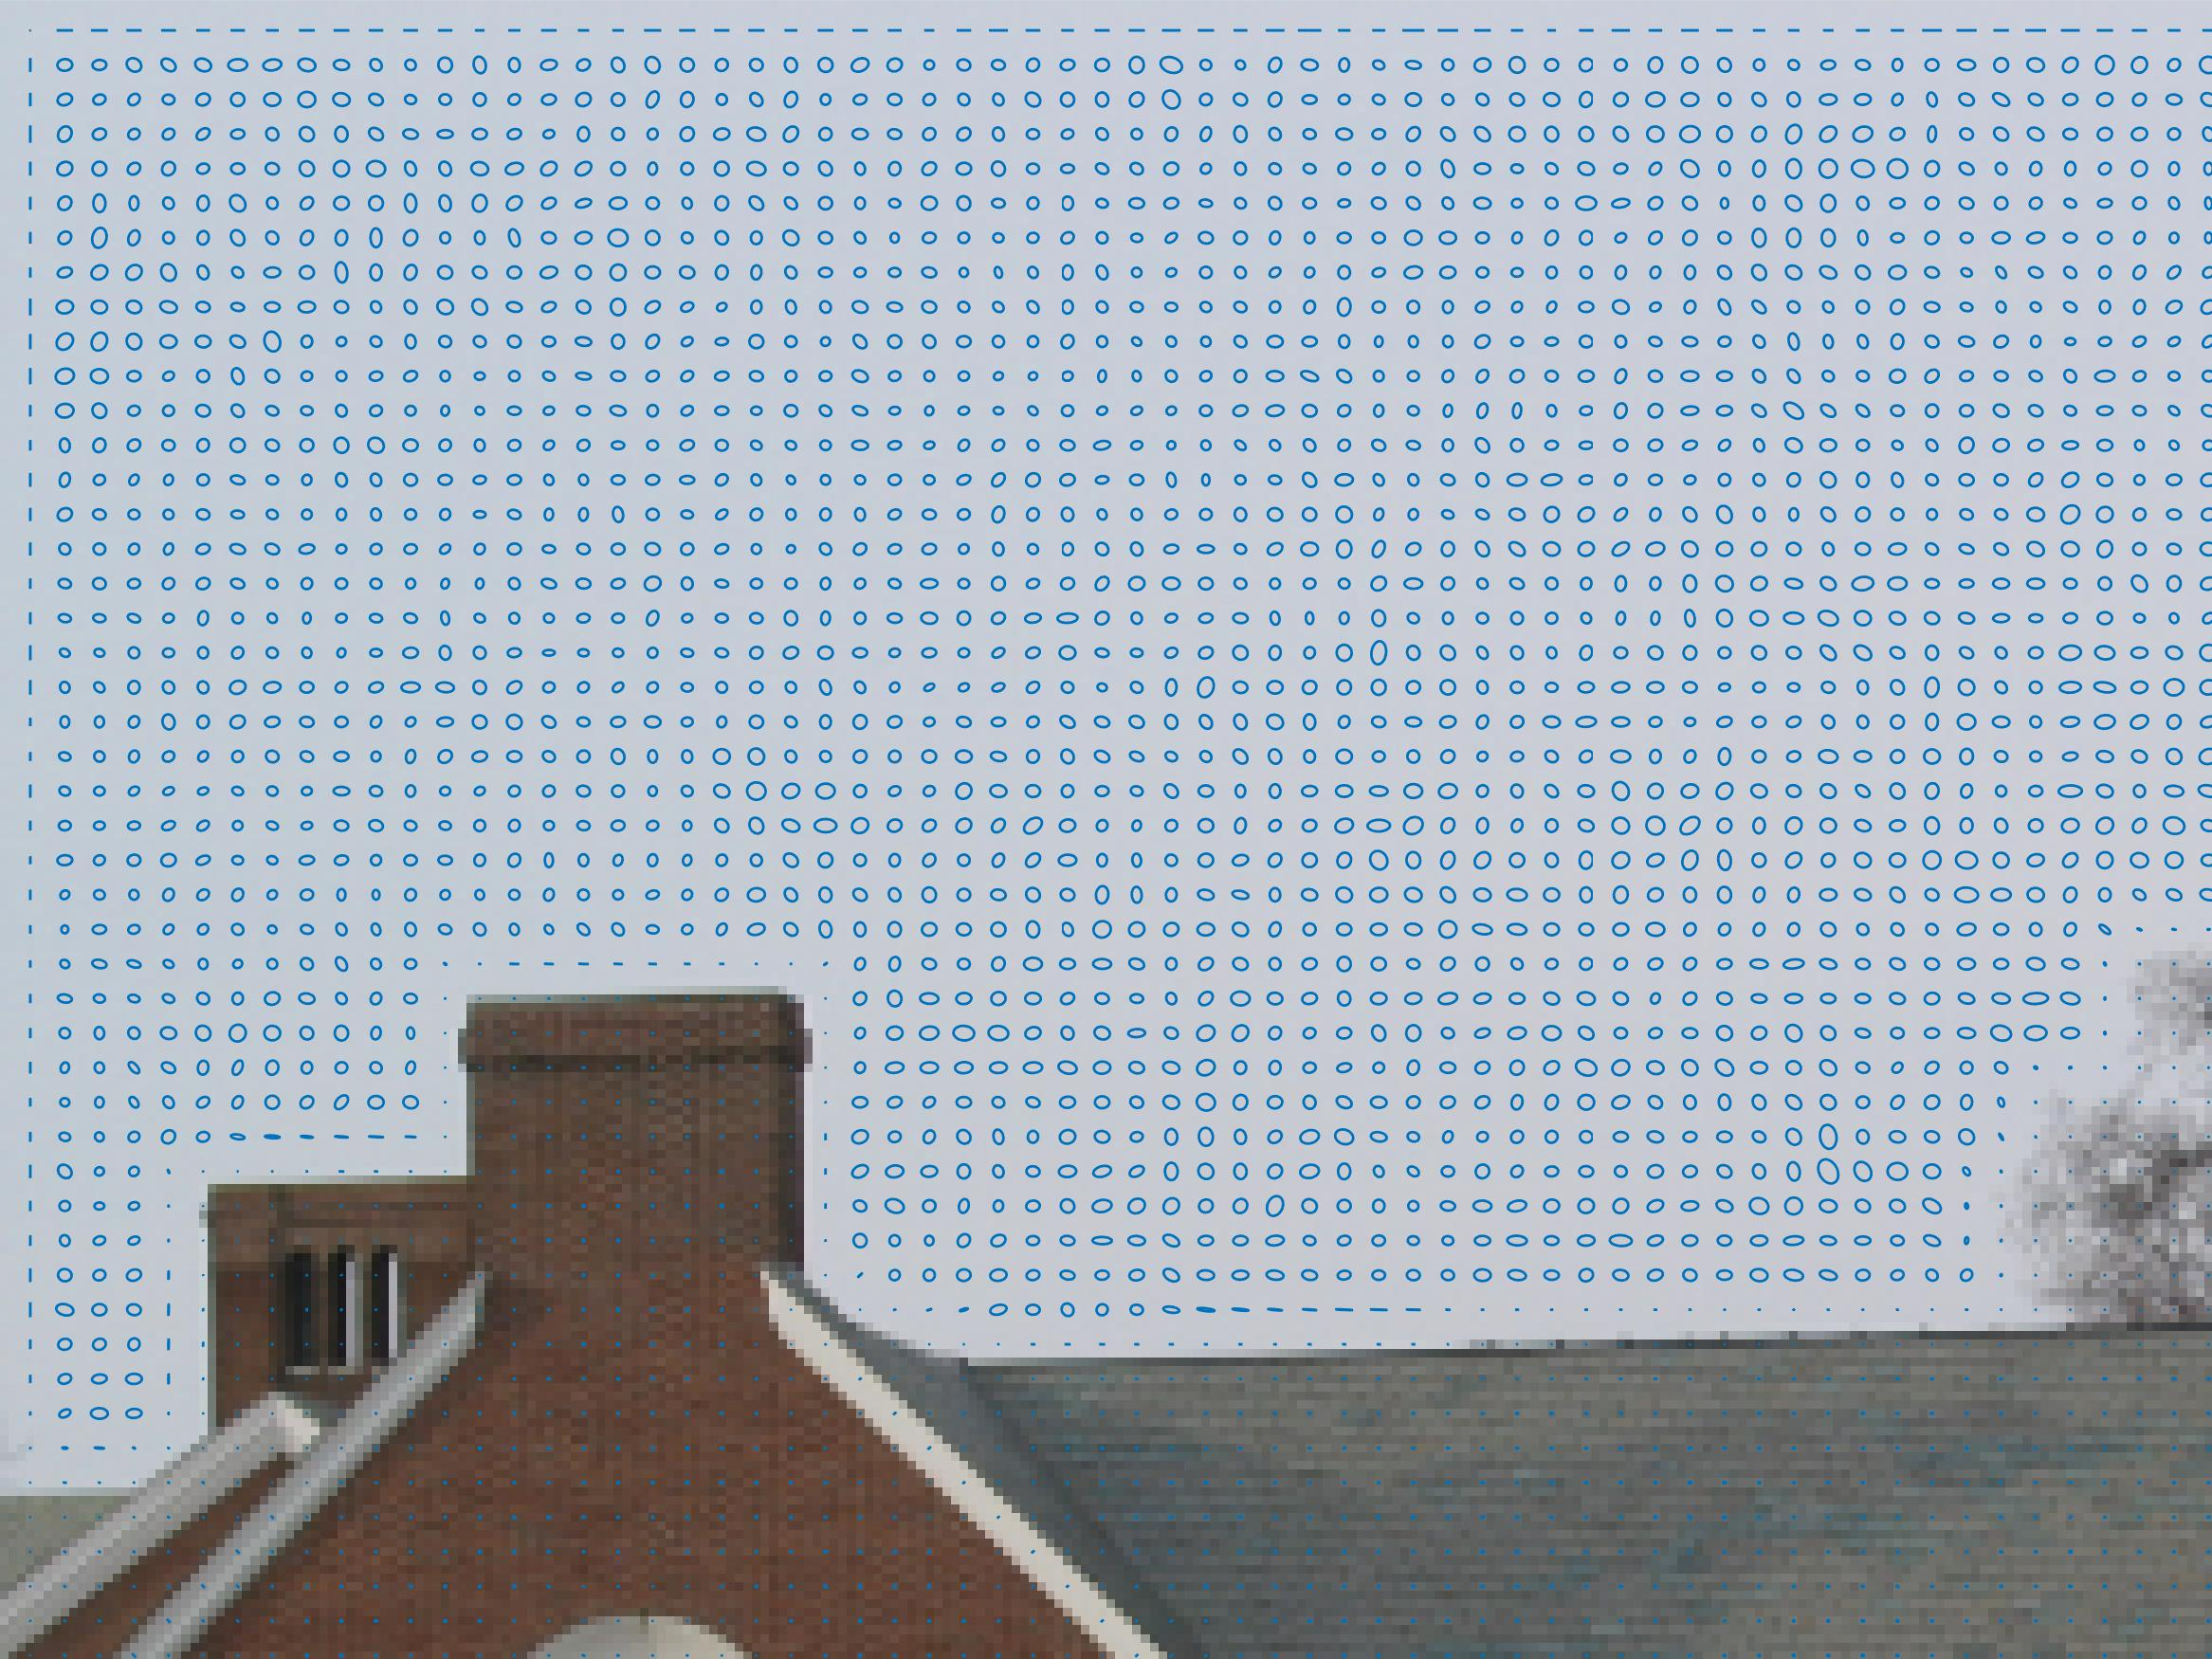
\includegraphics[width=0.9\columnwidth]{HW4_q1_b_w_9_I1.jpeg}
}
\subfigure[Result for I3.png] { \label{q1_b_w_9_fig:b}
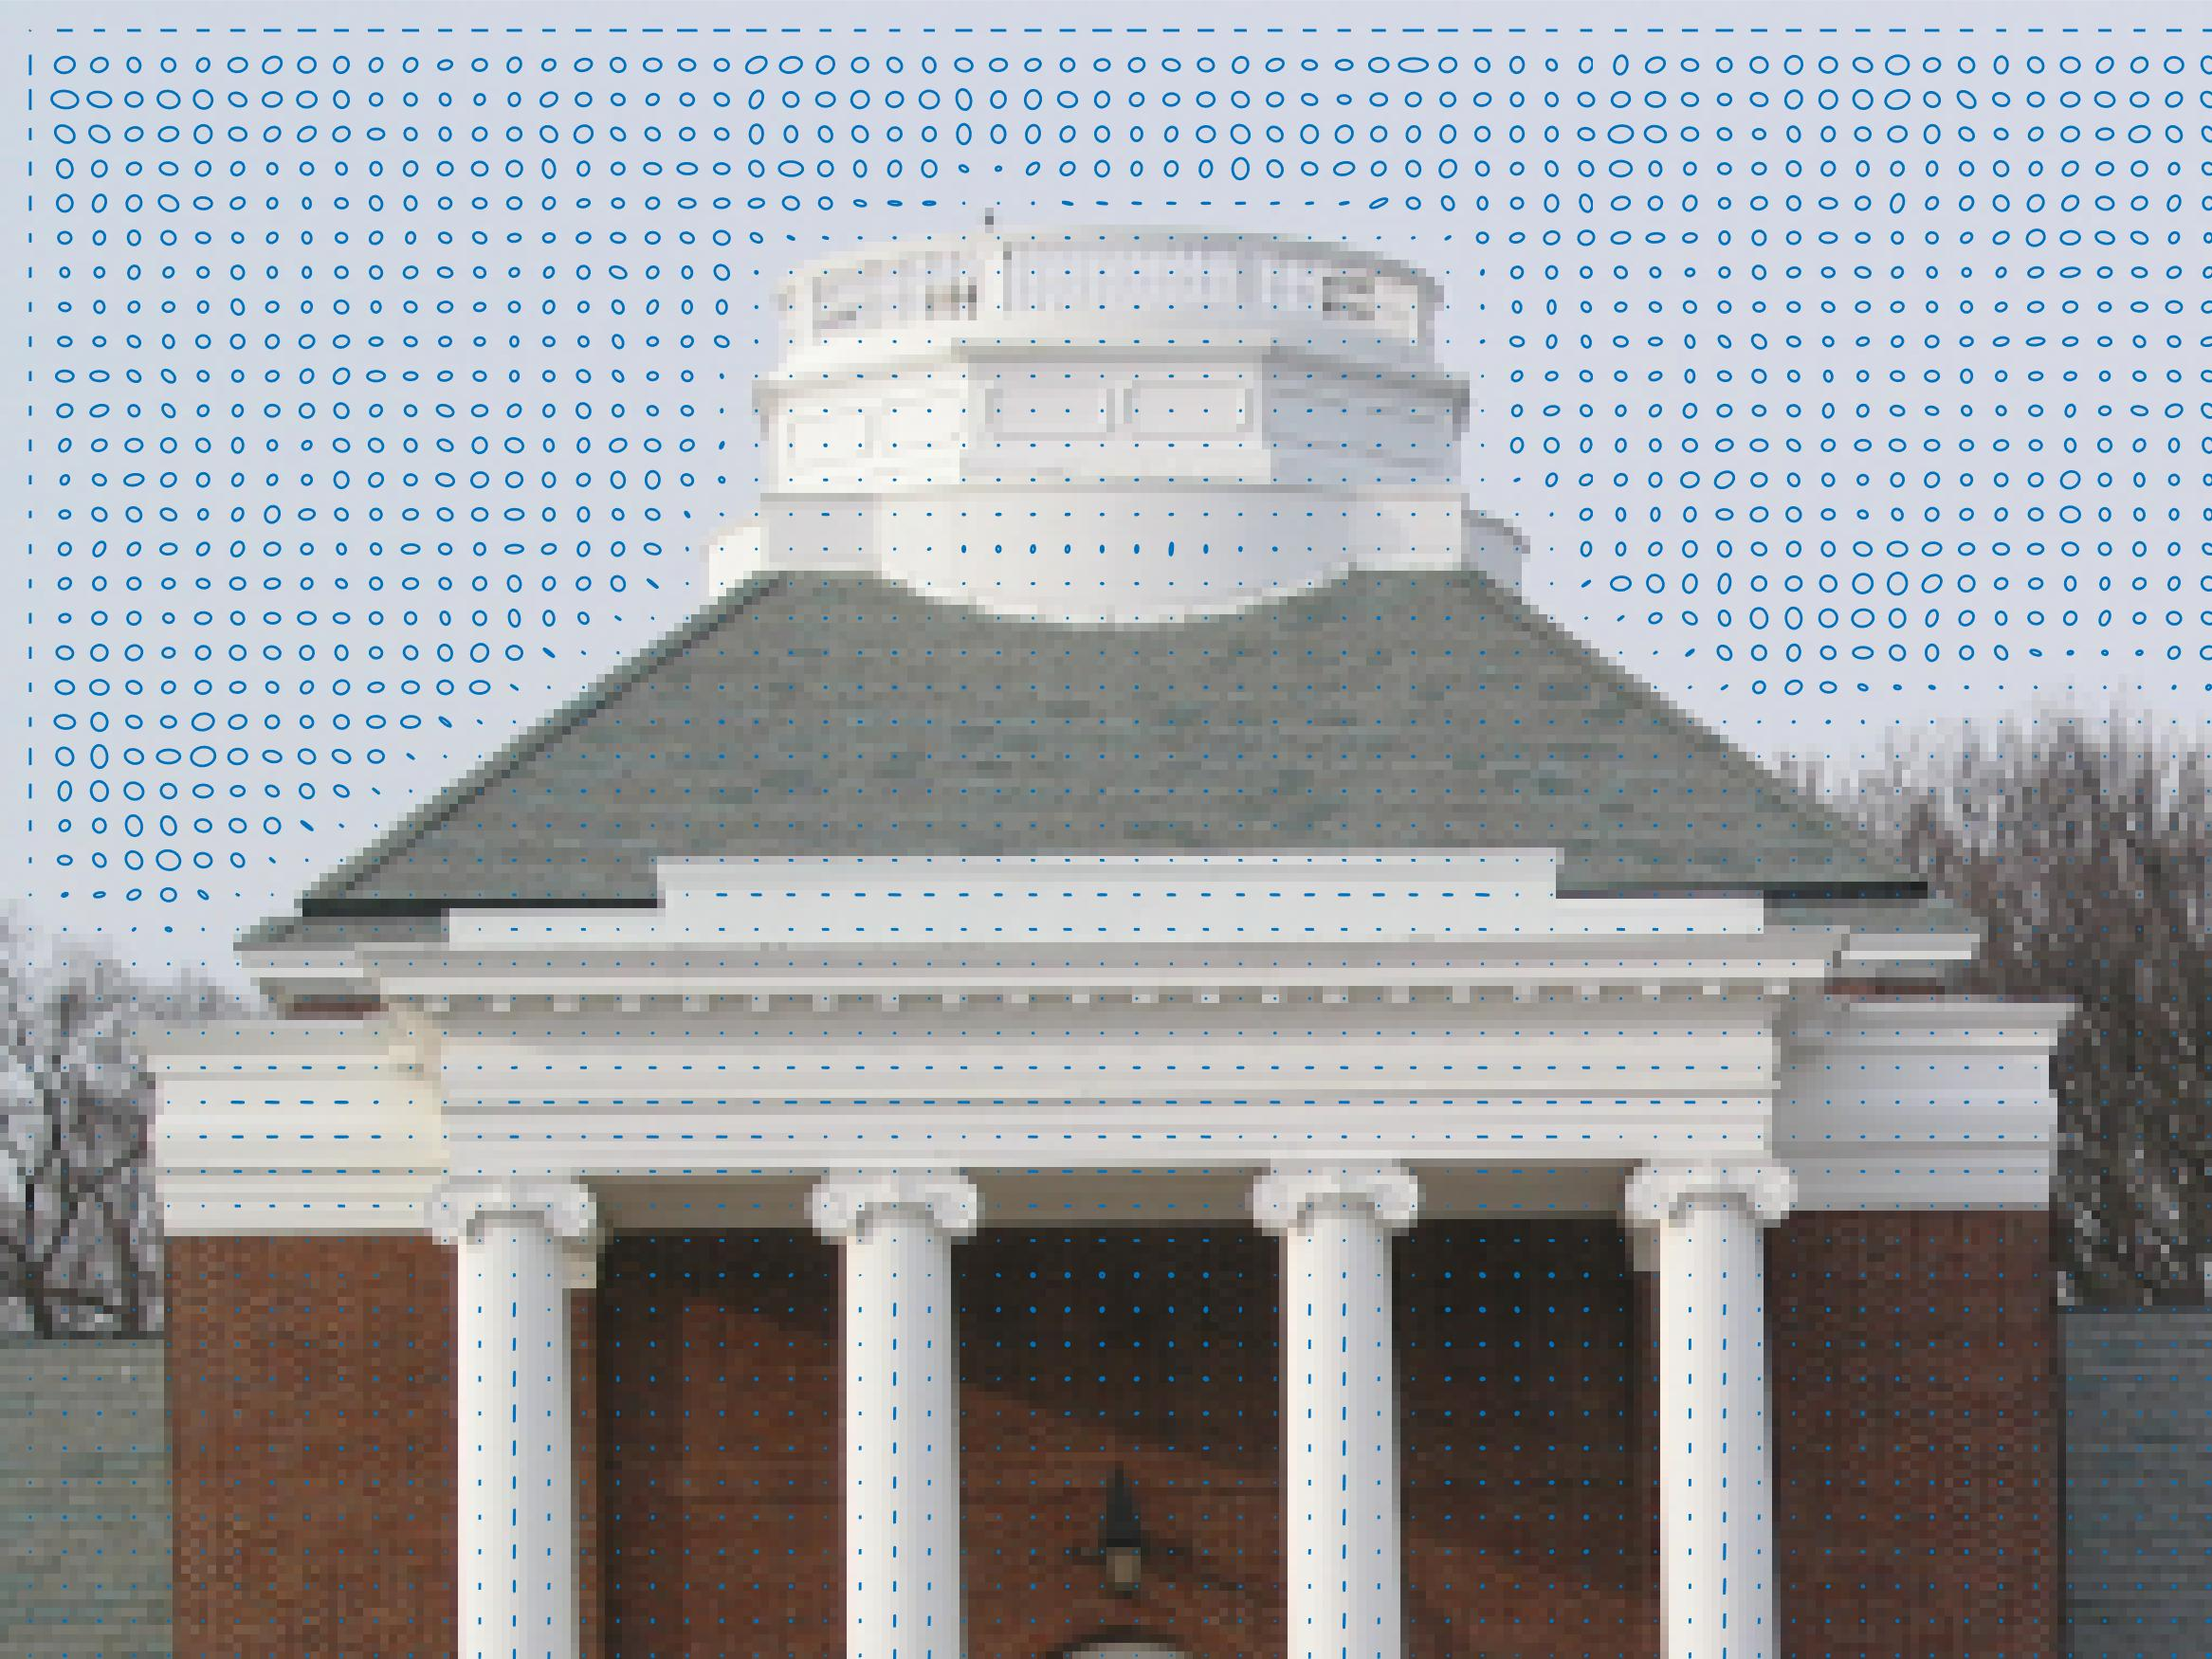
\includegraphics[width=0.9\columnwidth]{HW4_q1_b_w_9_I3.jpeg}
}
\caption{Superimpose Ellipses, $w=9$}
\label{q1_b_w_9}
\end{figure}


From figures above, we can see that while $w = 3$ gives ellipses with the most distinguishable shapes, and $w = 4$ gives reasonable result. However, the ellipses' changes are too small to be noticed when $w = 6$ and $w = 9$.\\

In conclusion, as window size becomes larger, the ellipses change would be more difficult to be observed.\\

Codes are attached below:\\
\begin{lstlisting}
%% EECS 442 - HW 04 - Q1 Harris Corner Detection
%  ------------------------------------------------------------------------
%  Date: 11 / 21 / 2016
%  Author: Fan Bu
%  ------------------------------------------------------------------------
%  ellipse(ra,rb,ang,x0,y0,C,Nb)
%  ------------------------------------------------------------------------
%  Instructions(Latex code)
% Key steps of the algorithm:\\
% Step1, Compute magnitude of the x and y gradients at each pixel.\\
% Step2, Due to Harris, construct a Gaussian window M around each pixel.\\
% Step3, Compute $\lambda_s$ of second moment matrix $M$ \\
% Step4, Compute $R=det(M)-k(tr(M))^2$ \\
% Step5, Set proper threshold $T$ \\
% Step6, If $R> T$, a corner is detected; then, retain point of local maxima. \\
% Step7, Superpose corners on images.\\

%% Initialization
clear all;
close all;
clc;
%% ----------------------- Load data ----------------------------
img1 = imread('I1.png');
img2 = imread('I3.png');

img = img2;
w = 3; %choose window size

%% ------------ Part 1: compute M,R and ellipse parameter --------
% translate to gray image
gray_img = rgb2gray(img);
[height,width] = size(gray_img);
% initialize corner position
is_edge = zeros(height, width);
% initialize R score
R = zeros(height, width);

% applying sobel edge detector in the horizontal direction
fx = [-1 0 1;
    -1 0 1;
    -1 0 1];
Ix = filter2(fx,gray_img);
% applying sobel edge detector in the vertical direction
fy = [1 1 1;
    0 0 0;
    -1 -1 -1];
Iy = filter2(fy,gray_img);
% compute terms for second moment matrix M
Ix2 = Ix.^2;
Iy2 = Iy.^2;
Ixy = Ix.*Iy;

% perform gaussian filtering for eliminating noises
h= fspecial('gaussian',[w w],2);
Ix2 = filter2(h,Ix2);
Iy2 = filter2(h,Iy2);
Ixy = filter2(h,Ixy);

% Initialize ellipsePerem
ellipsePerem = [];
Rmax = 0;
figure;
imshow(img(1:height/2,1:width/2,:),'border','tight','initialmagnification','fit');
hold on;
for i = 1:height
    for j = 1:width
        % compute second moment matrix M
        M = [
            Ix2(i,j), Ixy(i,j);
            Ixy(i,j) Iy2(i,j)
            ];
        % compute R(i,j) = det(M)-0.04*(trace(M))^2
        R(i,j) = det(M)-0.04*(trace(M))^2;
        if R(i,j) > Rmax
           Rmax = R(i,j);
        end;

    end;
end;
num_edge = 0;
Rmax
T=0.1*Rmax
% determine corner by comparing with threshold and all neighbor points
for i = 2:height-1
    for j = 2:width-1
        M = [
                 Ix2(i,j), Ixy(i,j);
                 Ixy(i,j) Iy2(i,j)
            ];
        % compute M's eigenvalue
        [vector,lambda] = eig(M);
        lambda = diag(lambda);
        % compute radius associate to the ellipse
        [lambda1,index] = max(lambda);
        lambda2 = min(lambda);
        a = lambda1^(-0.5);
        b = lambda2^(-0.5);
        vector = vector(:,index);
        angle = atan(vector(2)/vector(1));
        % form an ellipsePerem
        if mod(i,4) == 0 && mod(j,4) == 0
            ellipsePerem = [ellipsePerem;a b angle j i];
        end
        if R(i,j) > T ...
            && R(i,j) > R(i-1,j-1) ...
            && R(i,j) > R(i-1,j) ...
            && R(i,j) > R(i-1,j+1) ...
            && R(i,j) > R(i,j-1) ...
            && R(i,j) > R(i,j+1) ...
            && R(i,j) > R(i+1,j-1) ...
            && R(i,j) > R(i+1,j) ...
            && R(i,j) > R(i+1,j+1)

            is_edge(i,j) = 1;
            num_edge = num_edge+1;
        end;
    end;
end;
[edge_col, edge_row] = find(is_edge == 1);
num_edge
%% ========== Part 2: Plot ellipse and corner on image ====================

ellipse(ellipsePerem(:,1), ellipsePerem(:,2), ellipsePerem(:,3), ...
    ellipsePerem(:,4),ellipsePerem(:,5));
print(gcf,'-djpeg' ,['HW4_q1_b_w_',num2str(w),'_I3.jpeg'],'-r400')
\end{lstlisting}

\subsection*{(c)}
The thresholds are chosen as $T = t\cdot R_{max}$, where $R_{max}$ is defined as the maximum corner response and takes value of $9.4191\times 10^9$ for I1.png, and $1.0741\times 10^{10}$ for I3.png.\\

Take $t = 0.001, 0.01, 0.05, 0.1$, and the results are shown in figures \ref{q1_c_t_001},\ref{q1_c_t_01},\ref{q1_c_t_05},\ref{q1_c_t_1}:\\

\begin{figure}[H] \centering
\subfigure[$t=0.001$ for I1.png] { \label{q1_c_t_001_fig:a}
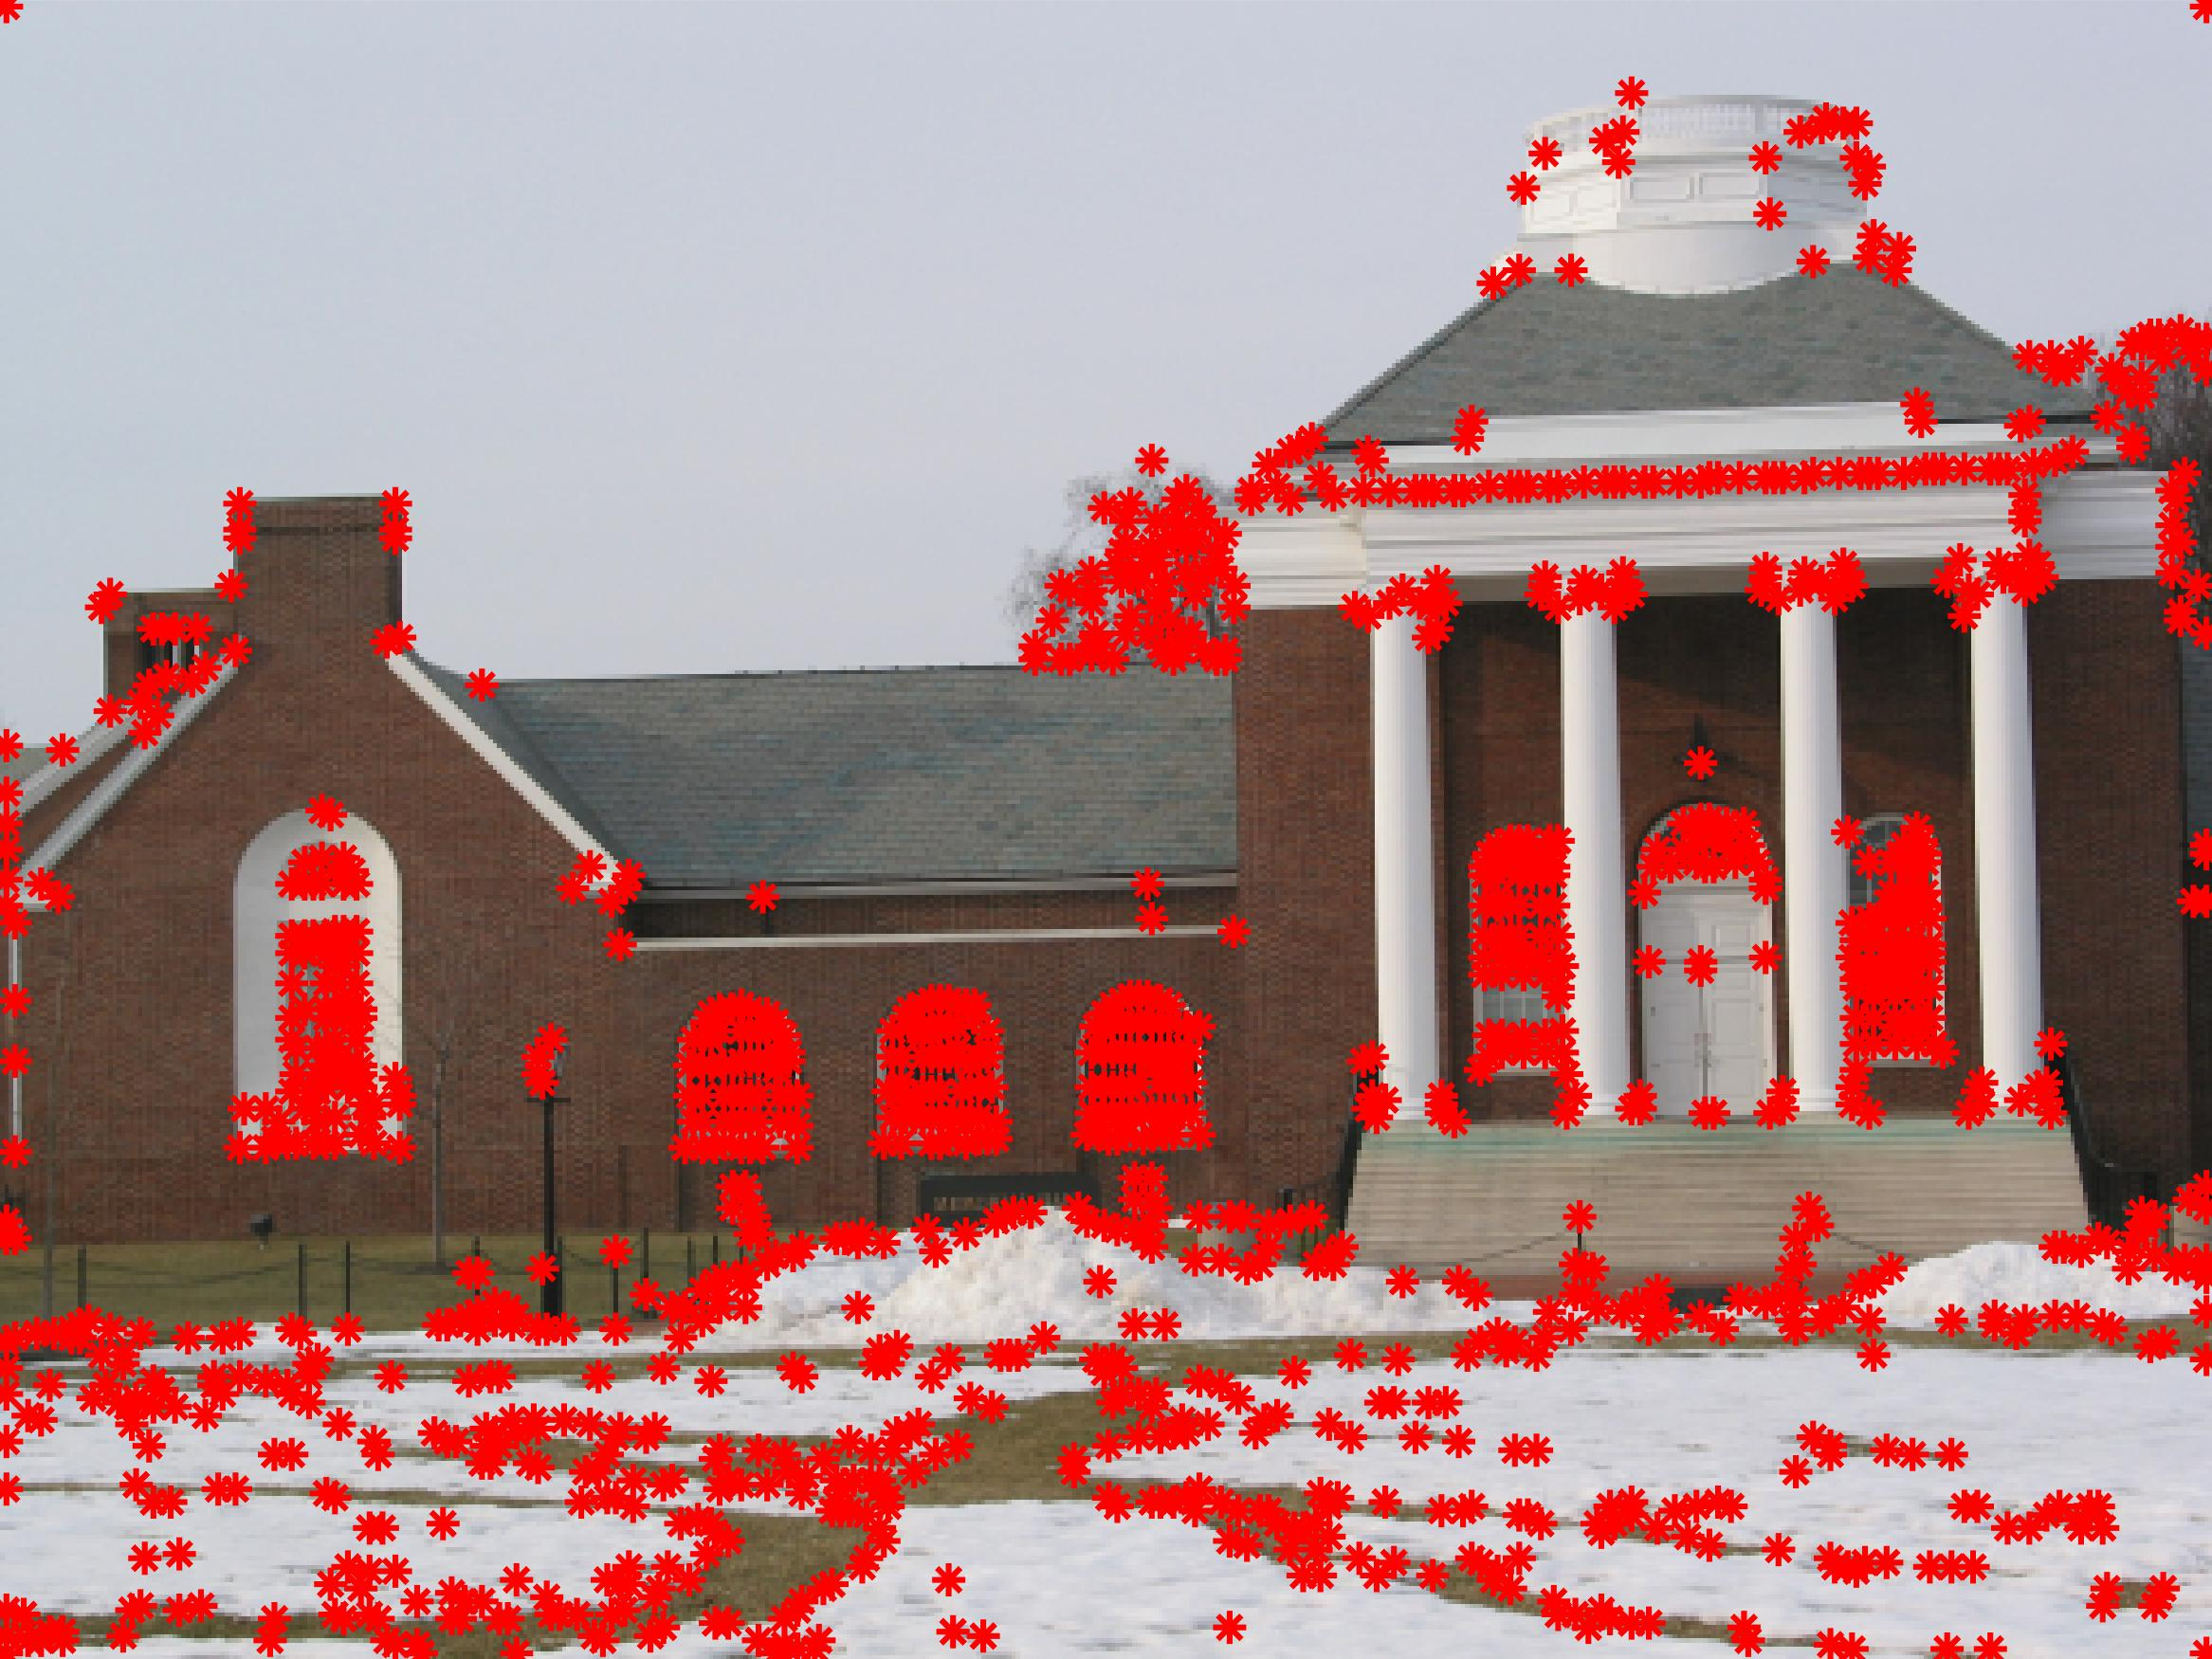
\includegraphics[width=0.45\columnwidth]{HW4_q1_c_t_001_I1.jpeg}
}
\subfigure[$t=0.001$ for I3.png] { \label{q1_c_t_001_fig:b}
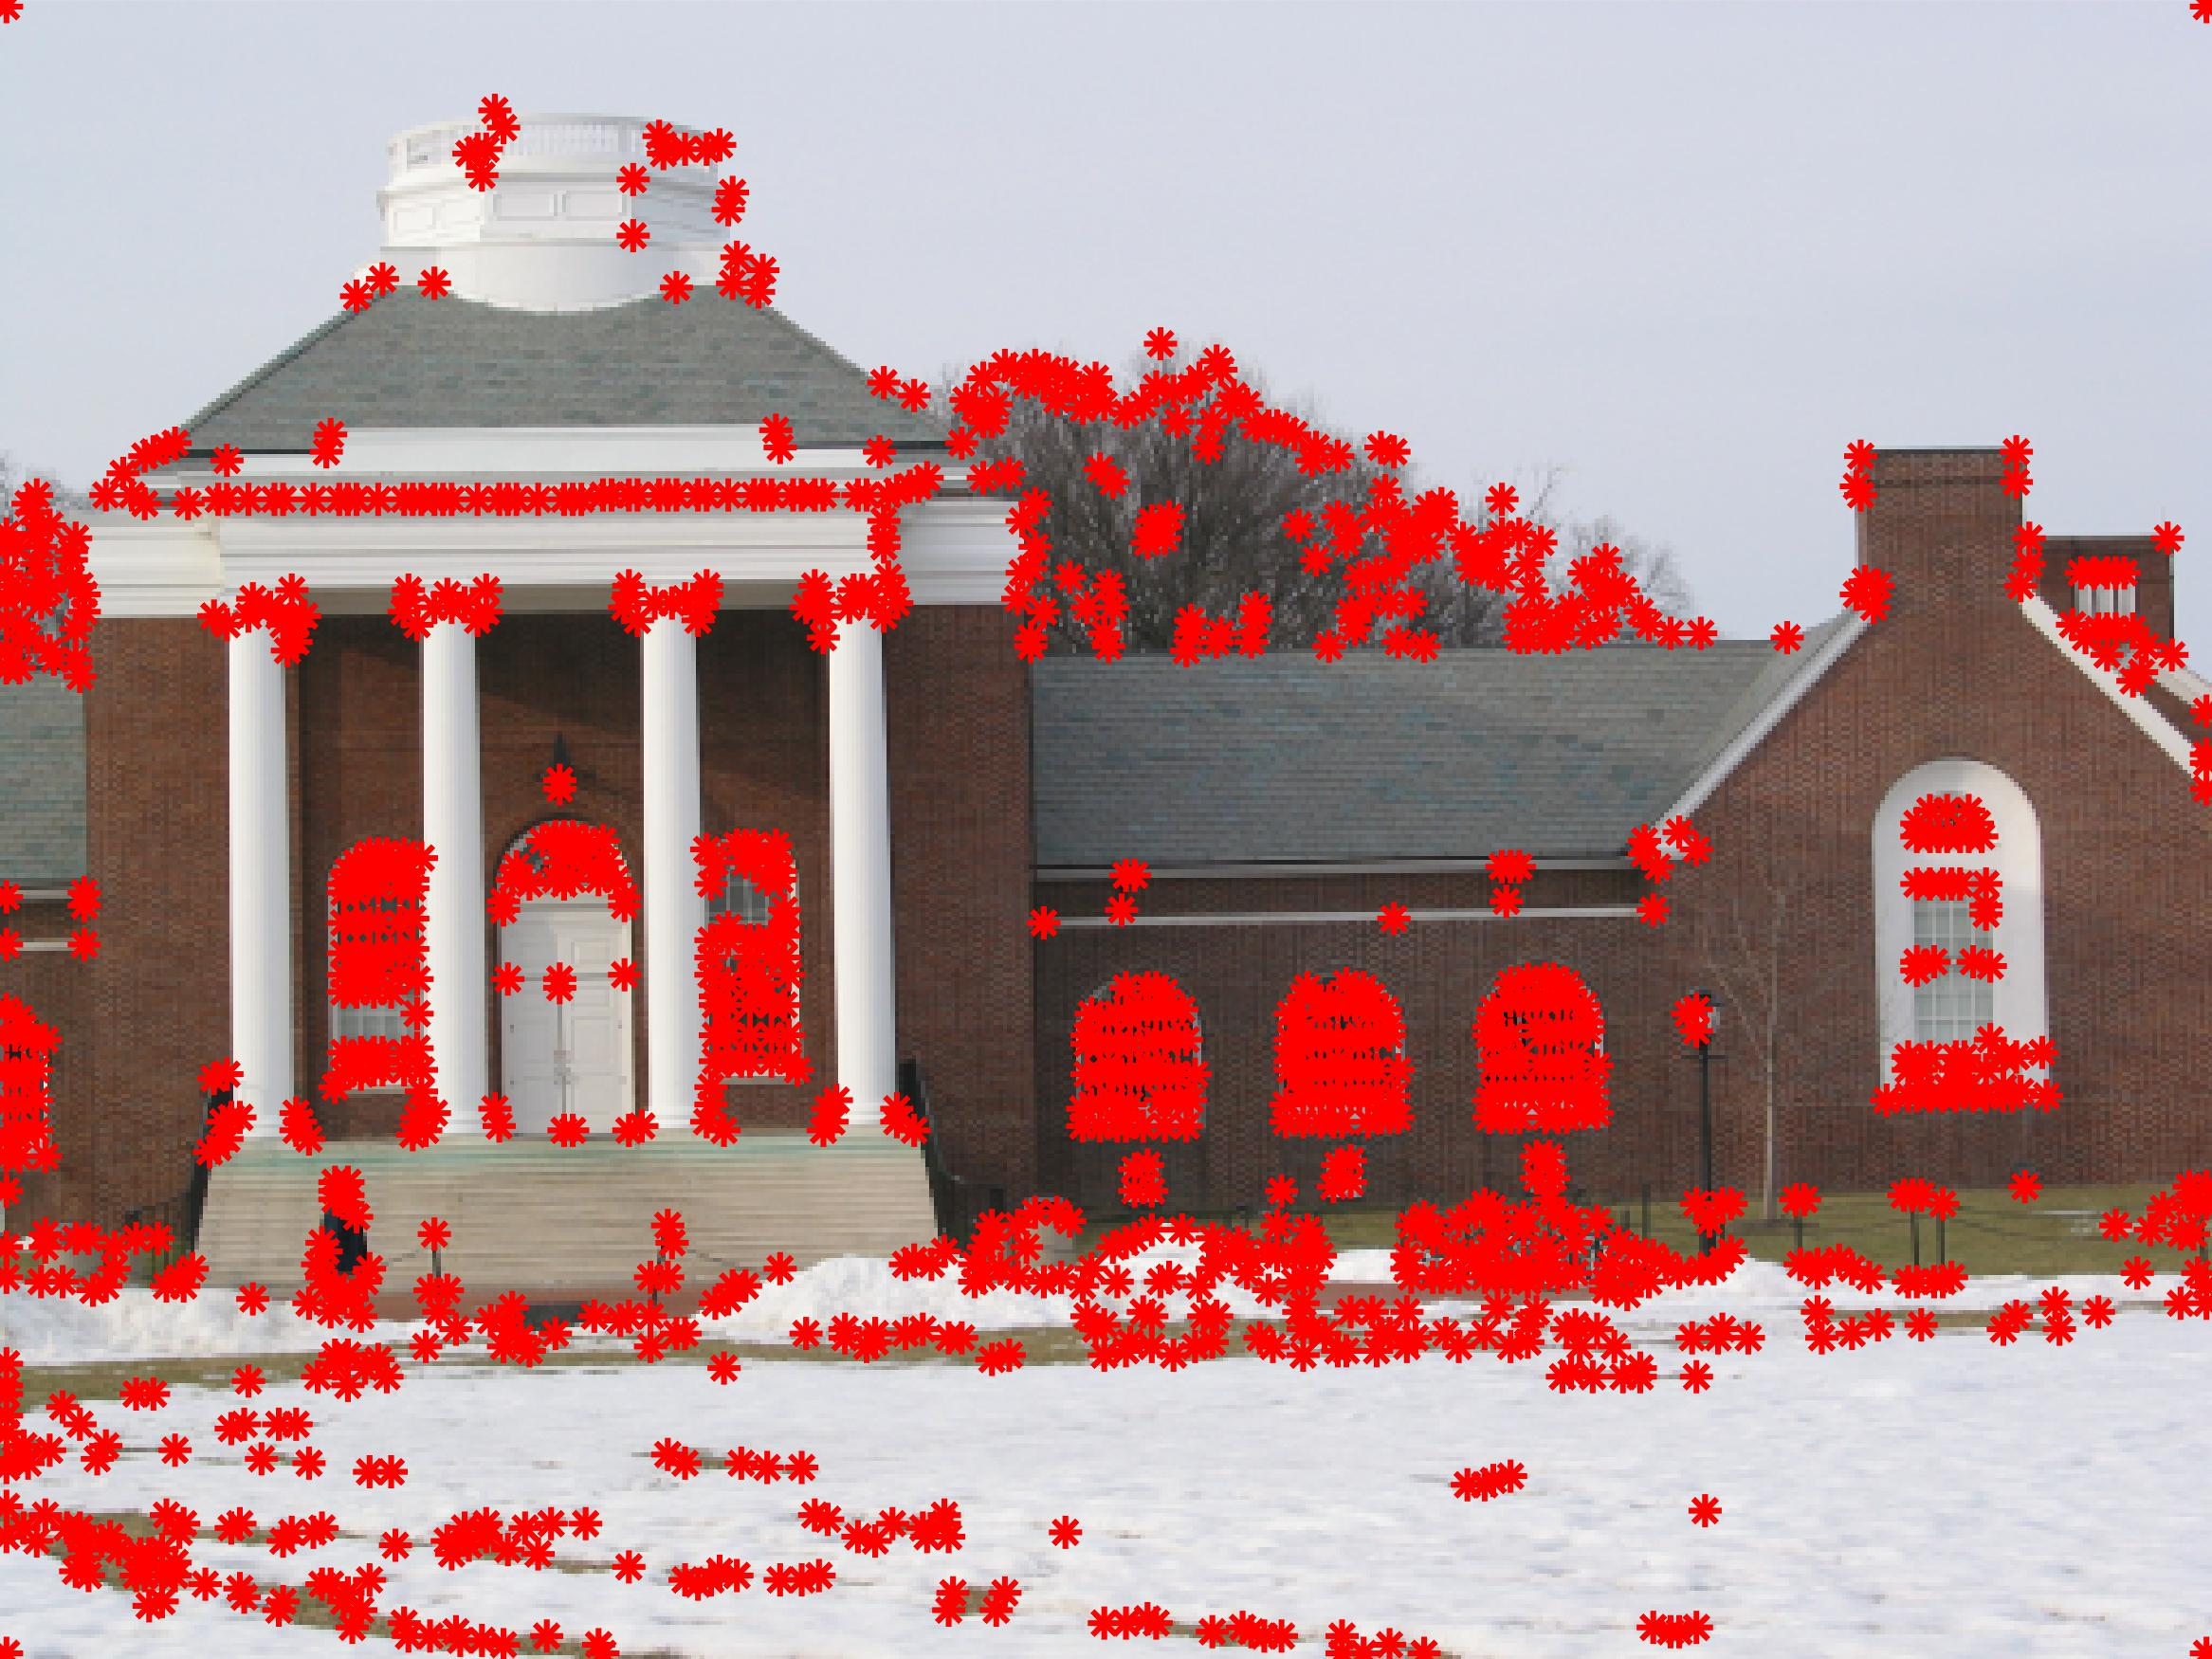
\includegraphics[width=0.45\columnwidth]{HW4_q1_c_t_001_I3.jpeg}
}
\caption{Harris Corner Detection results with different threshold, $T = tR_{max}, t=0.001$}
\label{q1_c_t_001}
\end{figure}

\begin{figure}[H] \centering
\subfigure[$t=0.01$ for I1.png] { \label{q1_c_t_01_fig:a}
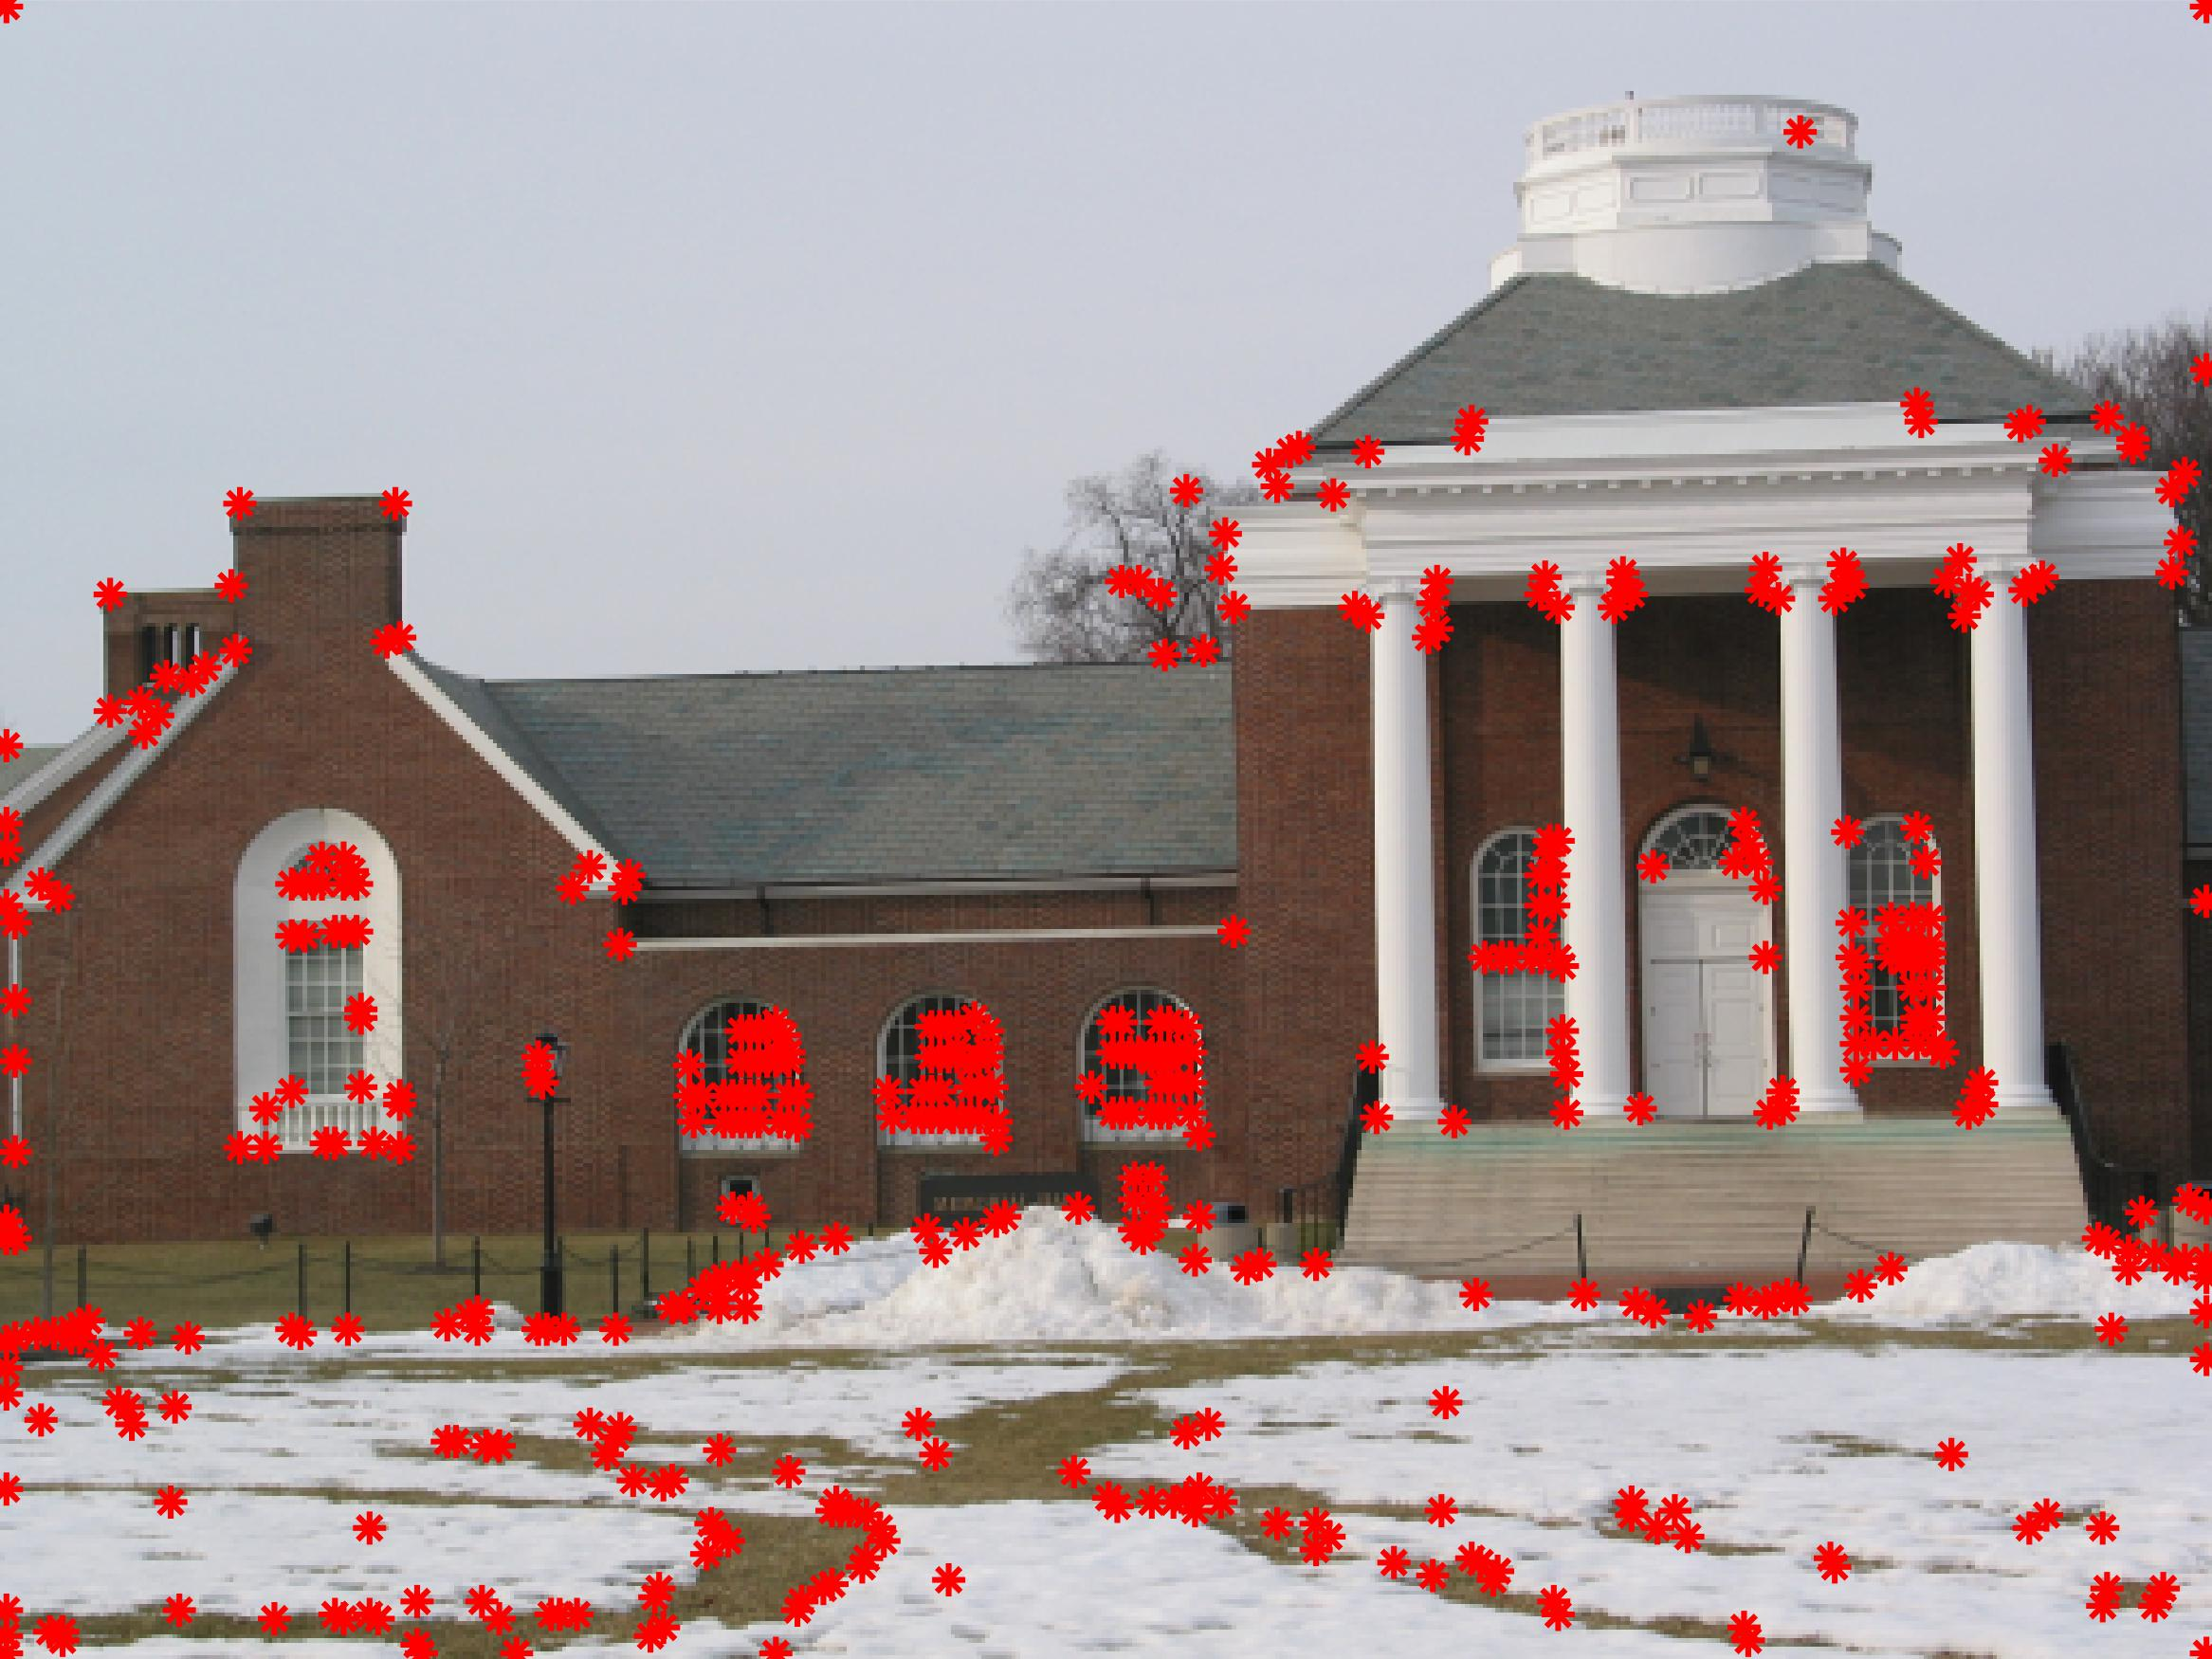
\includegraphics[width=0.45\columnwidth]{HW4_q1_c_t_01_I1.jpeg}
}
\subfigure[$t=0.01$ for I3.png] { \label{q1_c_t_01_fig:b}
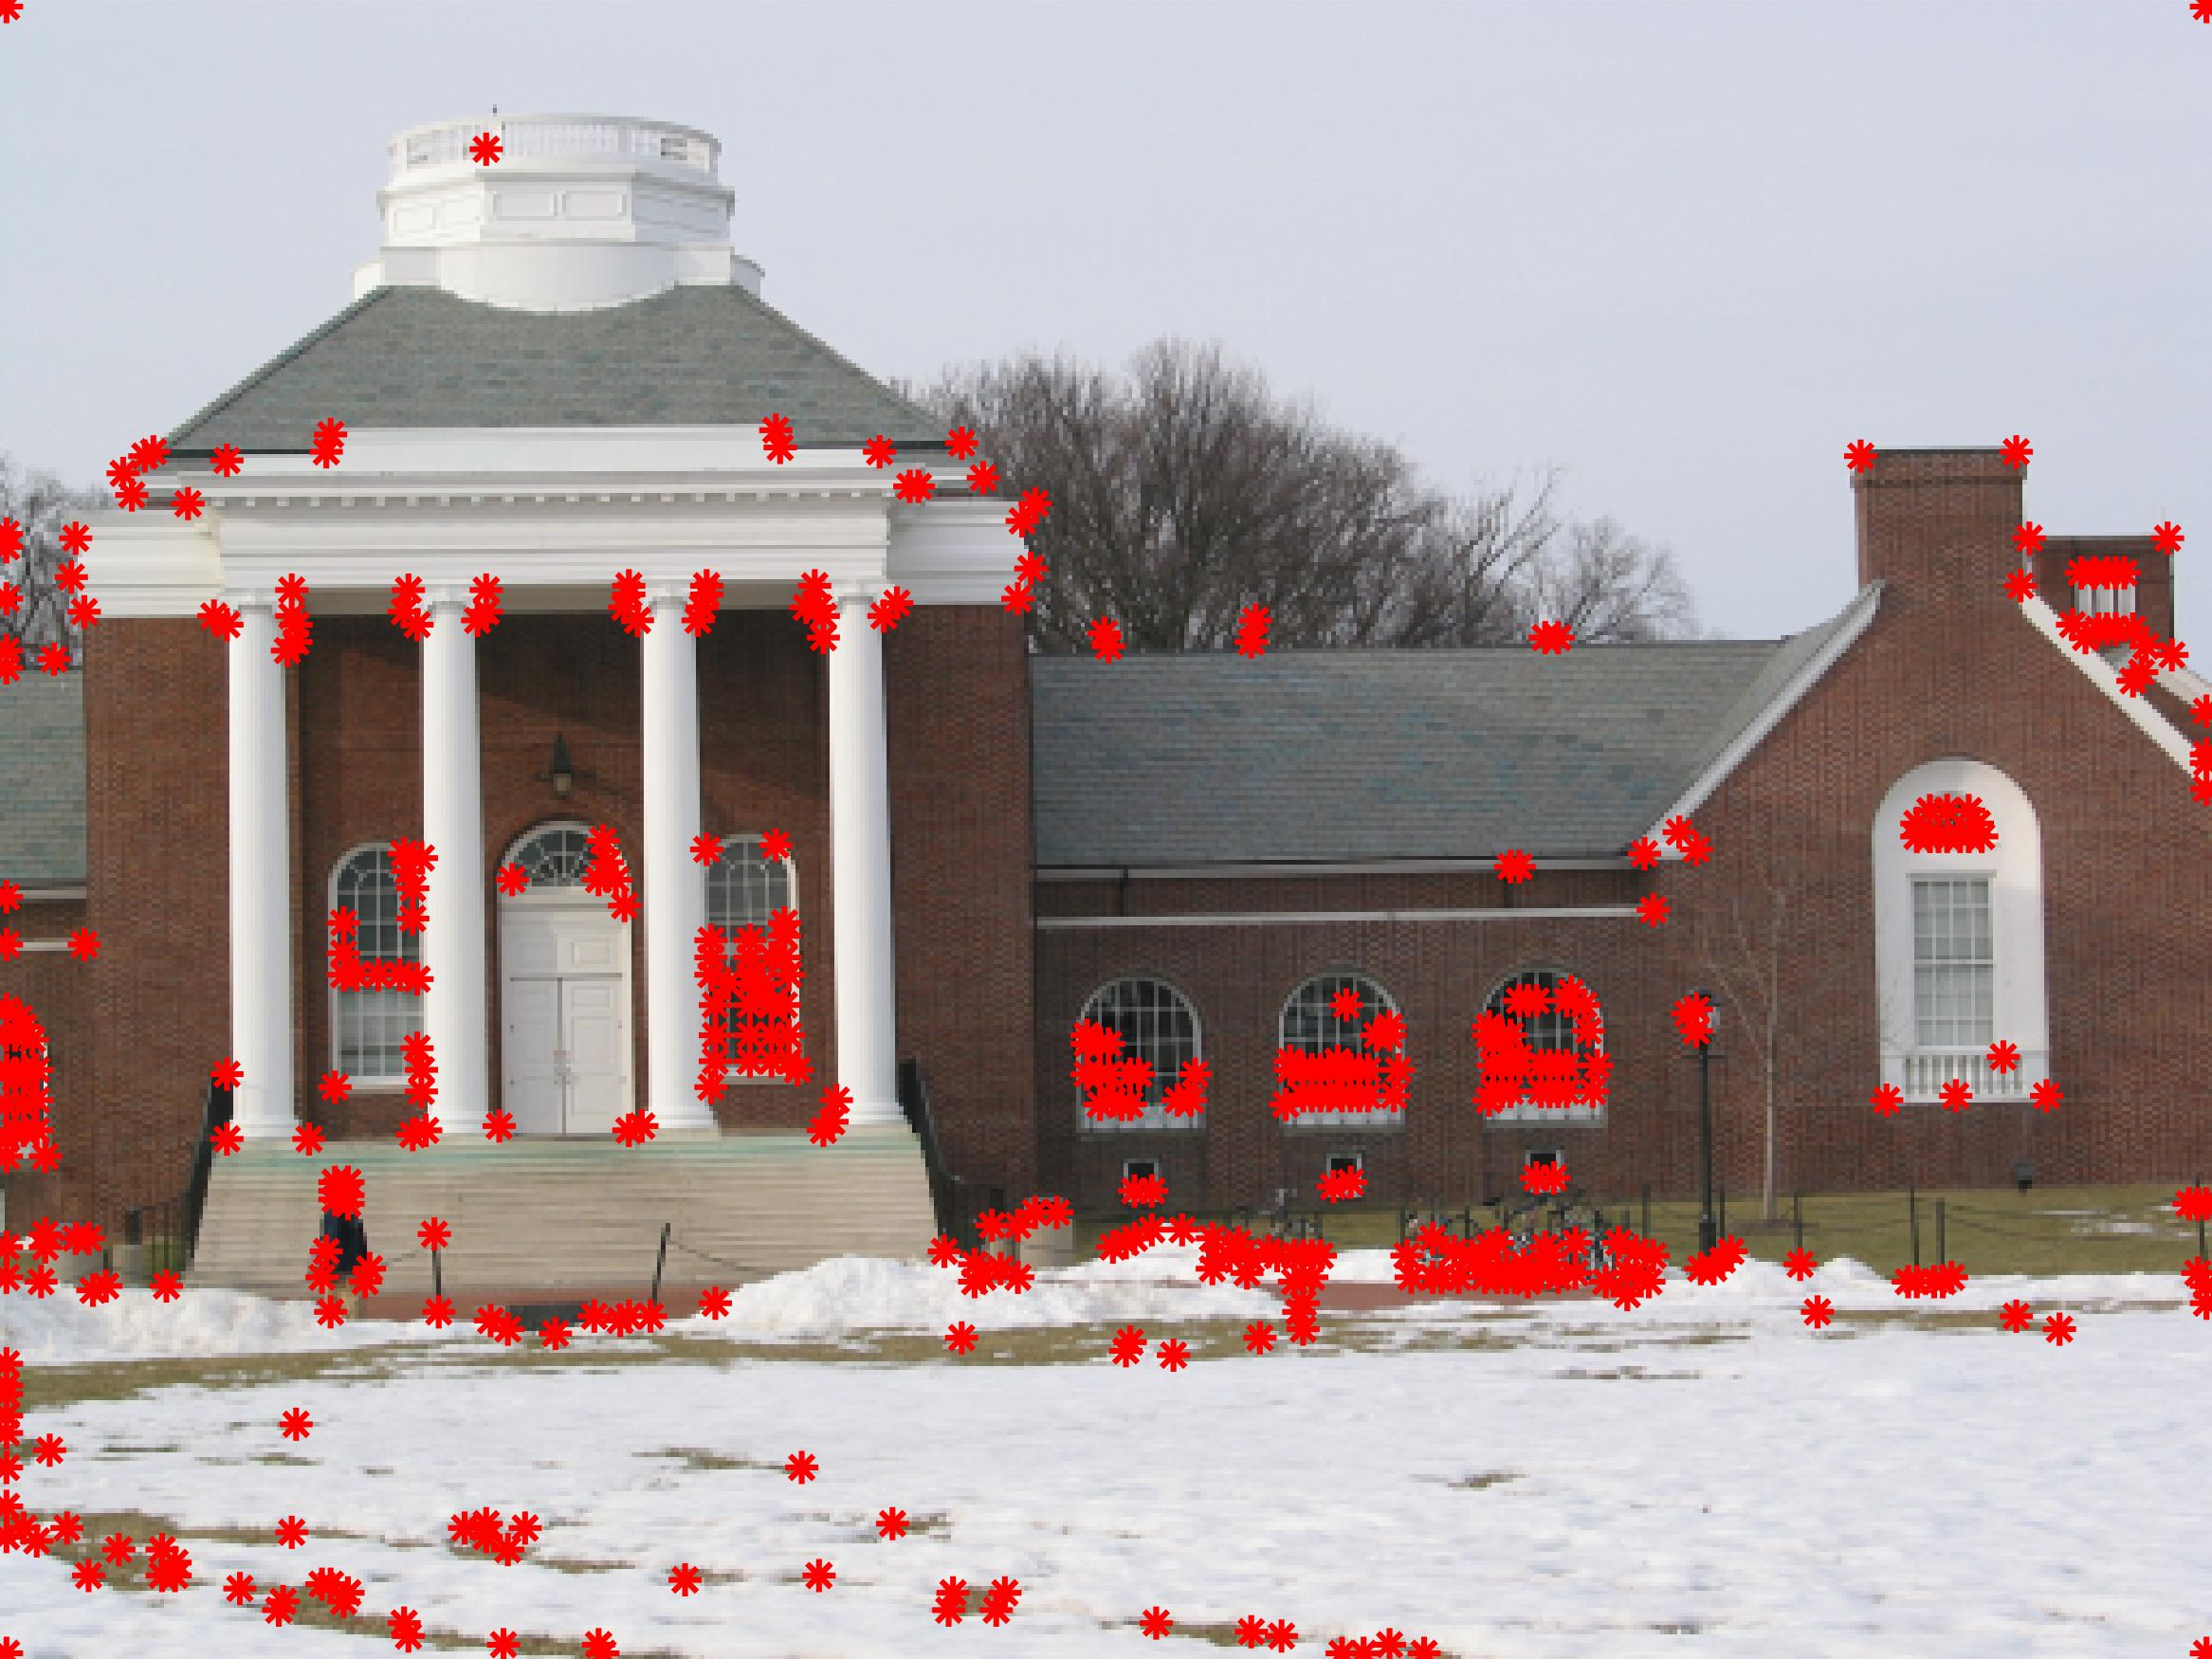
\includegraphics[width=0.45\columnwidth]{HW4_q1_c_t_01_I3.jpeg}
}
\caption{Harris Corner Detection results with different threshold, $T = tR_{max}, t=0.01$}
\label{q1_c_t_01}
\end{figure}

\begin{figure}[H] \centering
\subfigure[$t=0.05$ for I1.png] { \label{q1_c_t_05_fig:a}
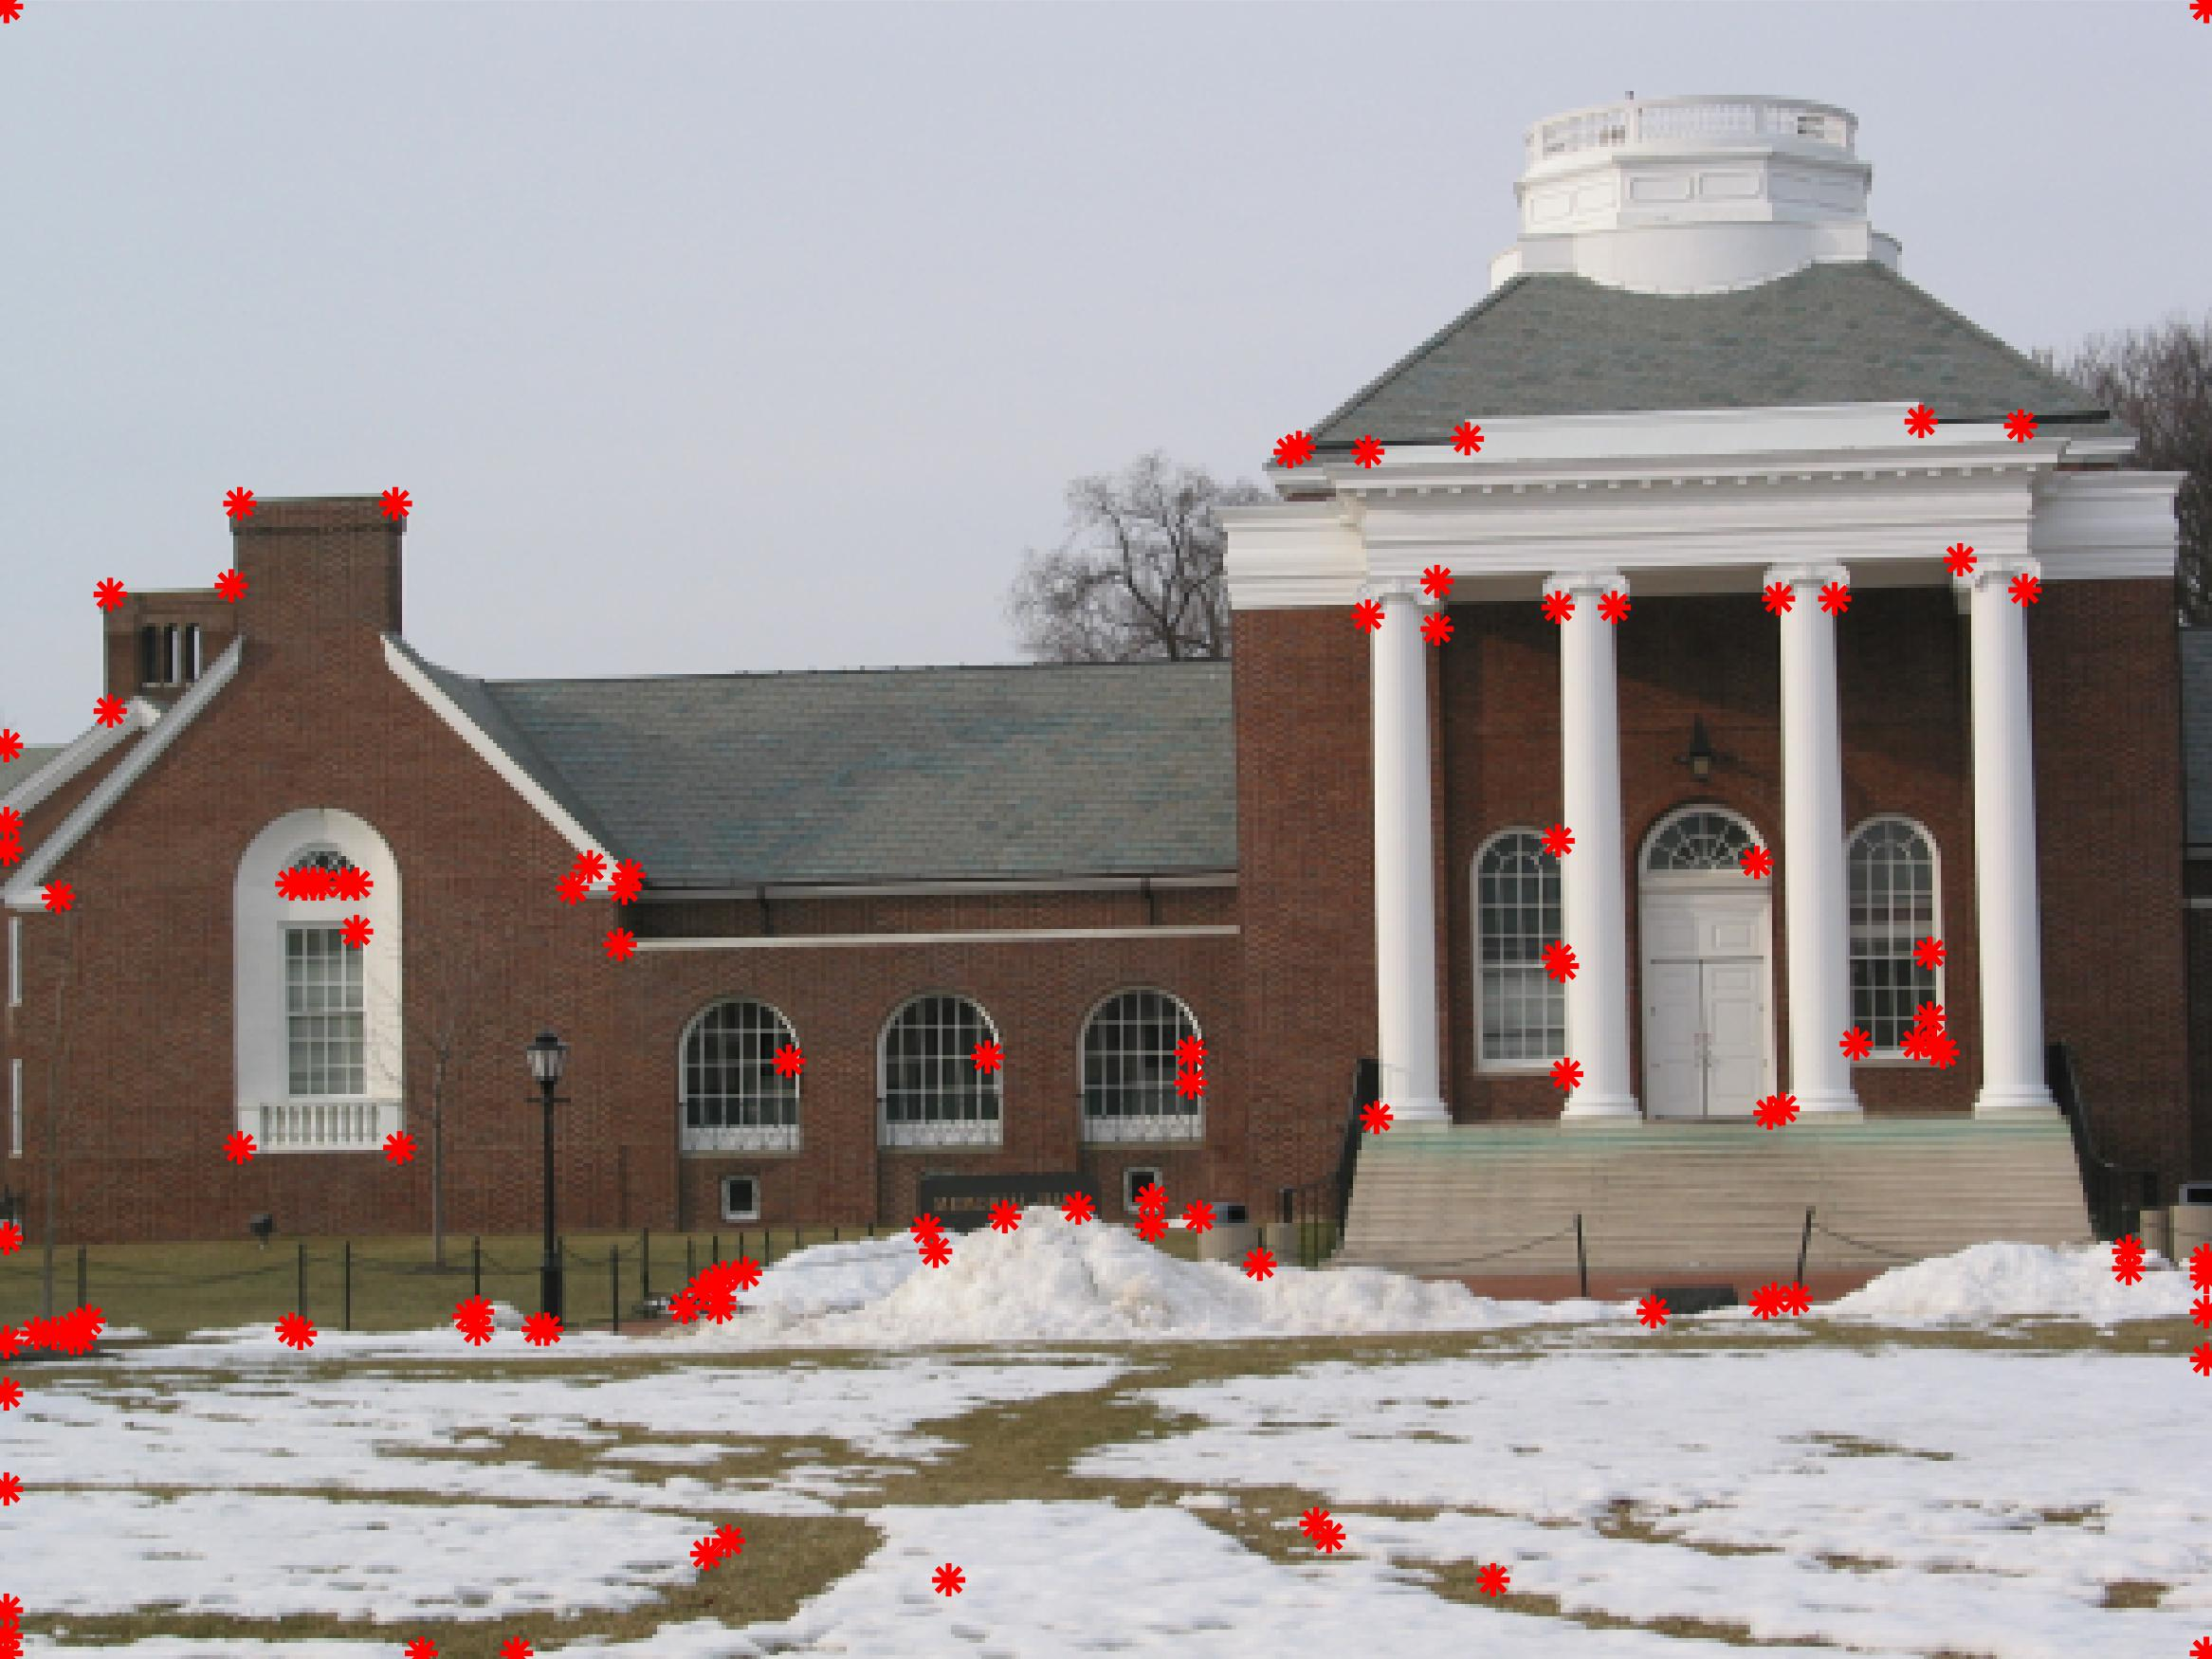
\includegraphics[width=0.45\columnwidth]{HW4_q1_c_t_05_I1.jpeg}
}
\subfigure[$t=0.05$ for I3.png] { \label{q1_c_t_05_fig:b}
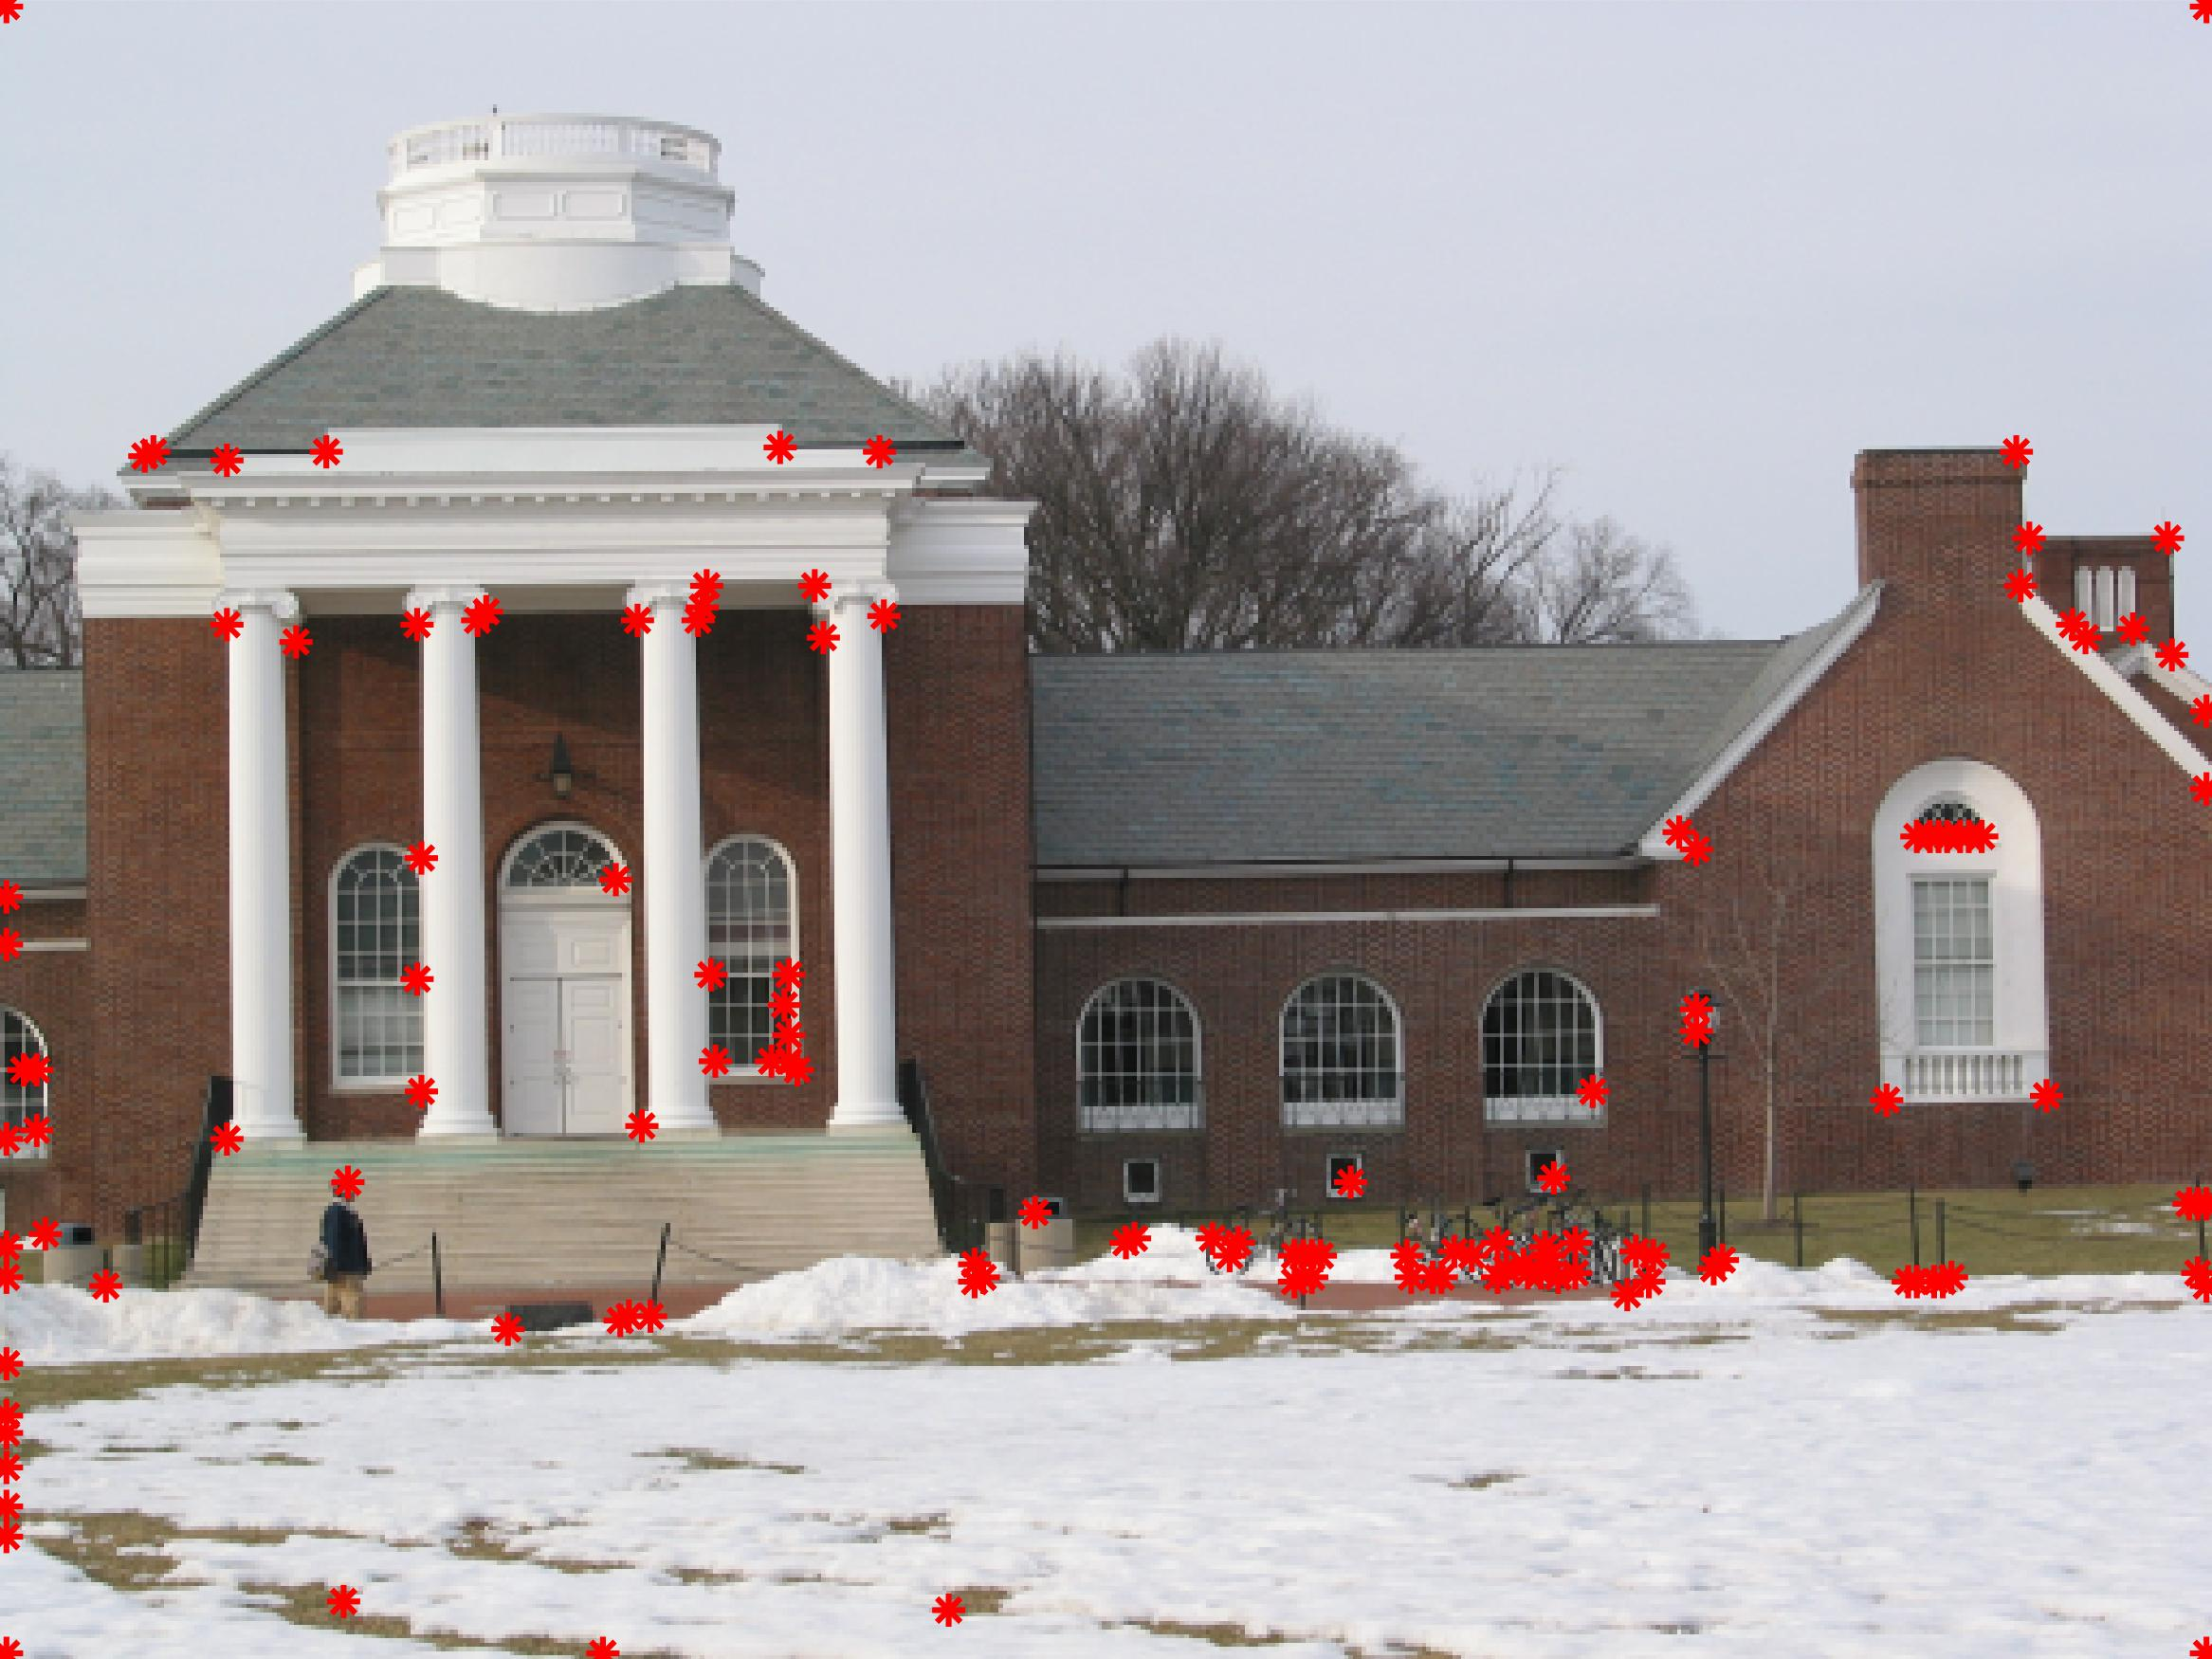
\includegraphics[width=0.45\columnwidth]{HW4_q1_c_t_05_I3.jpeg}
}
\caption{Harris Corner Detection results with different threshold, $T = tR_{max}, t=0.05$}
\label{q1_c_t_05}
\end{figure}

\begin{figure}[H] \centering
\subfigure[$t=0.1$ for I1.png] { \label{q1_c_t_1_fig:a}
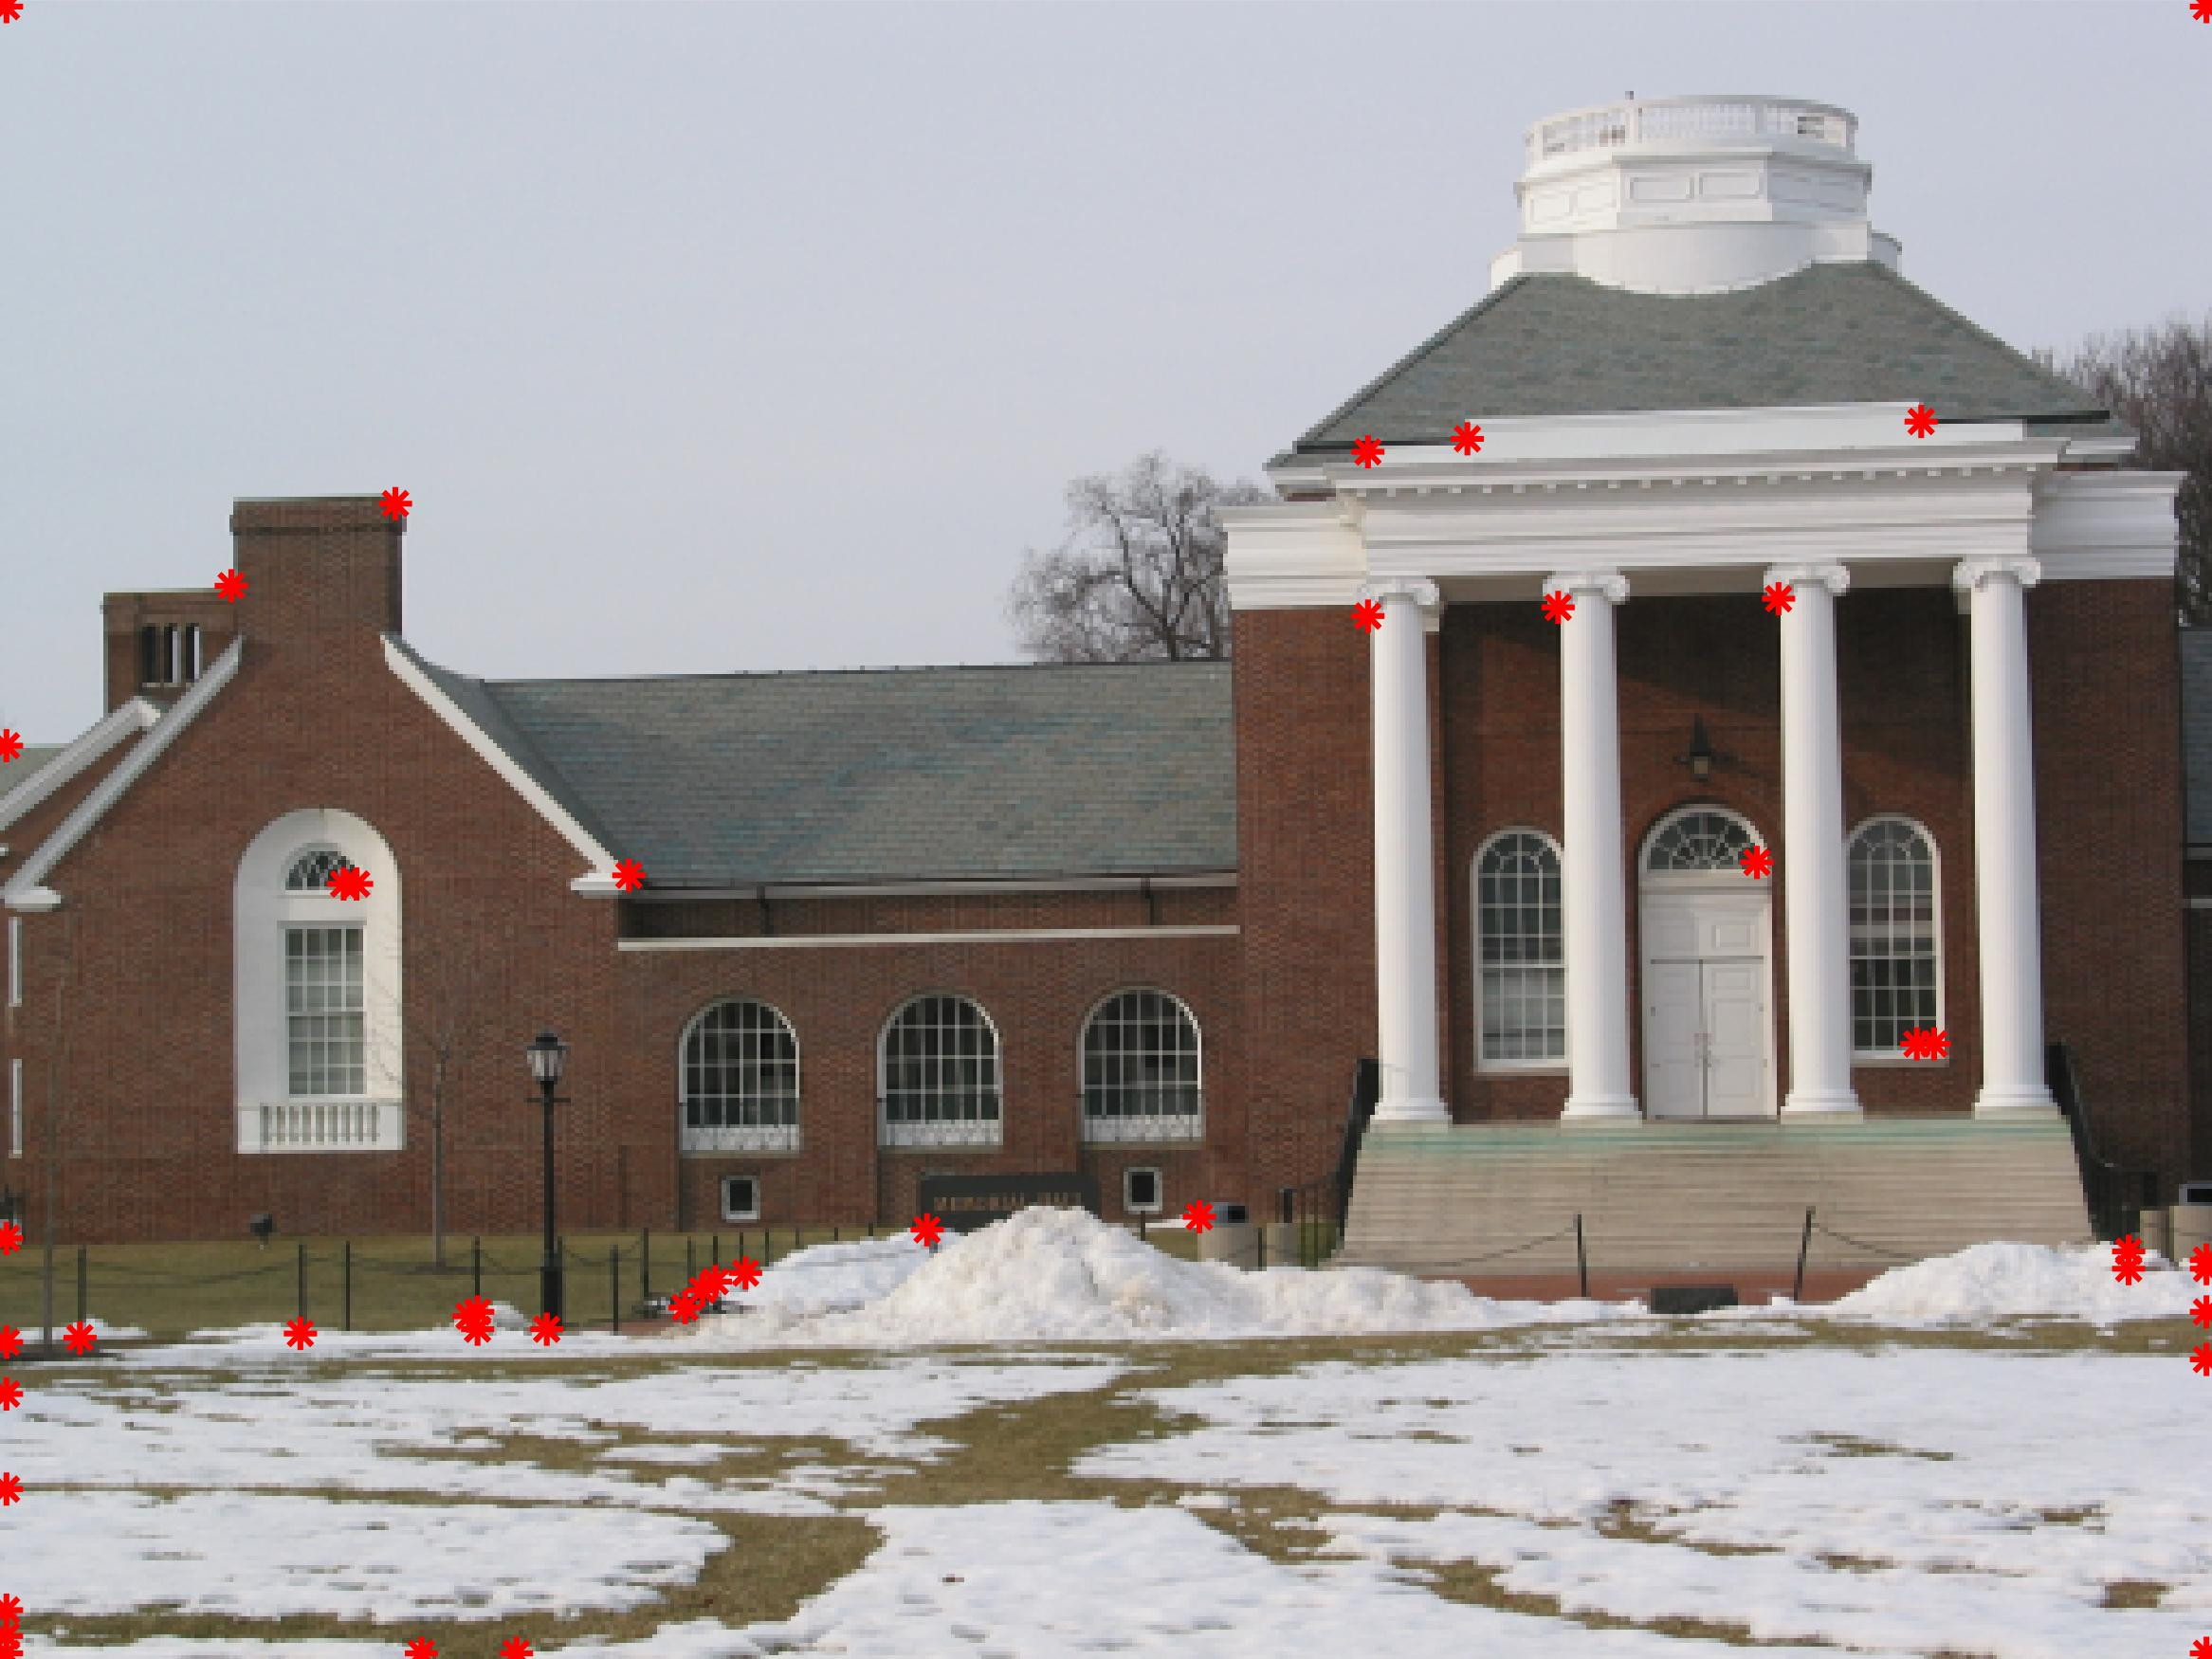
\includegraphics[width=0.45\columnwidth]{HW4_q1_c_t_1_I1.jpeg}
}
\subfigure[$t=0.1$ for I3.png] { \label{q1_c_t_1_fig:b}
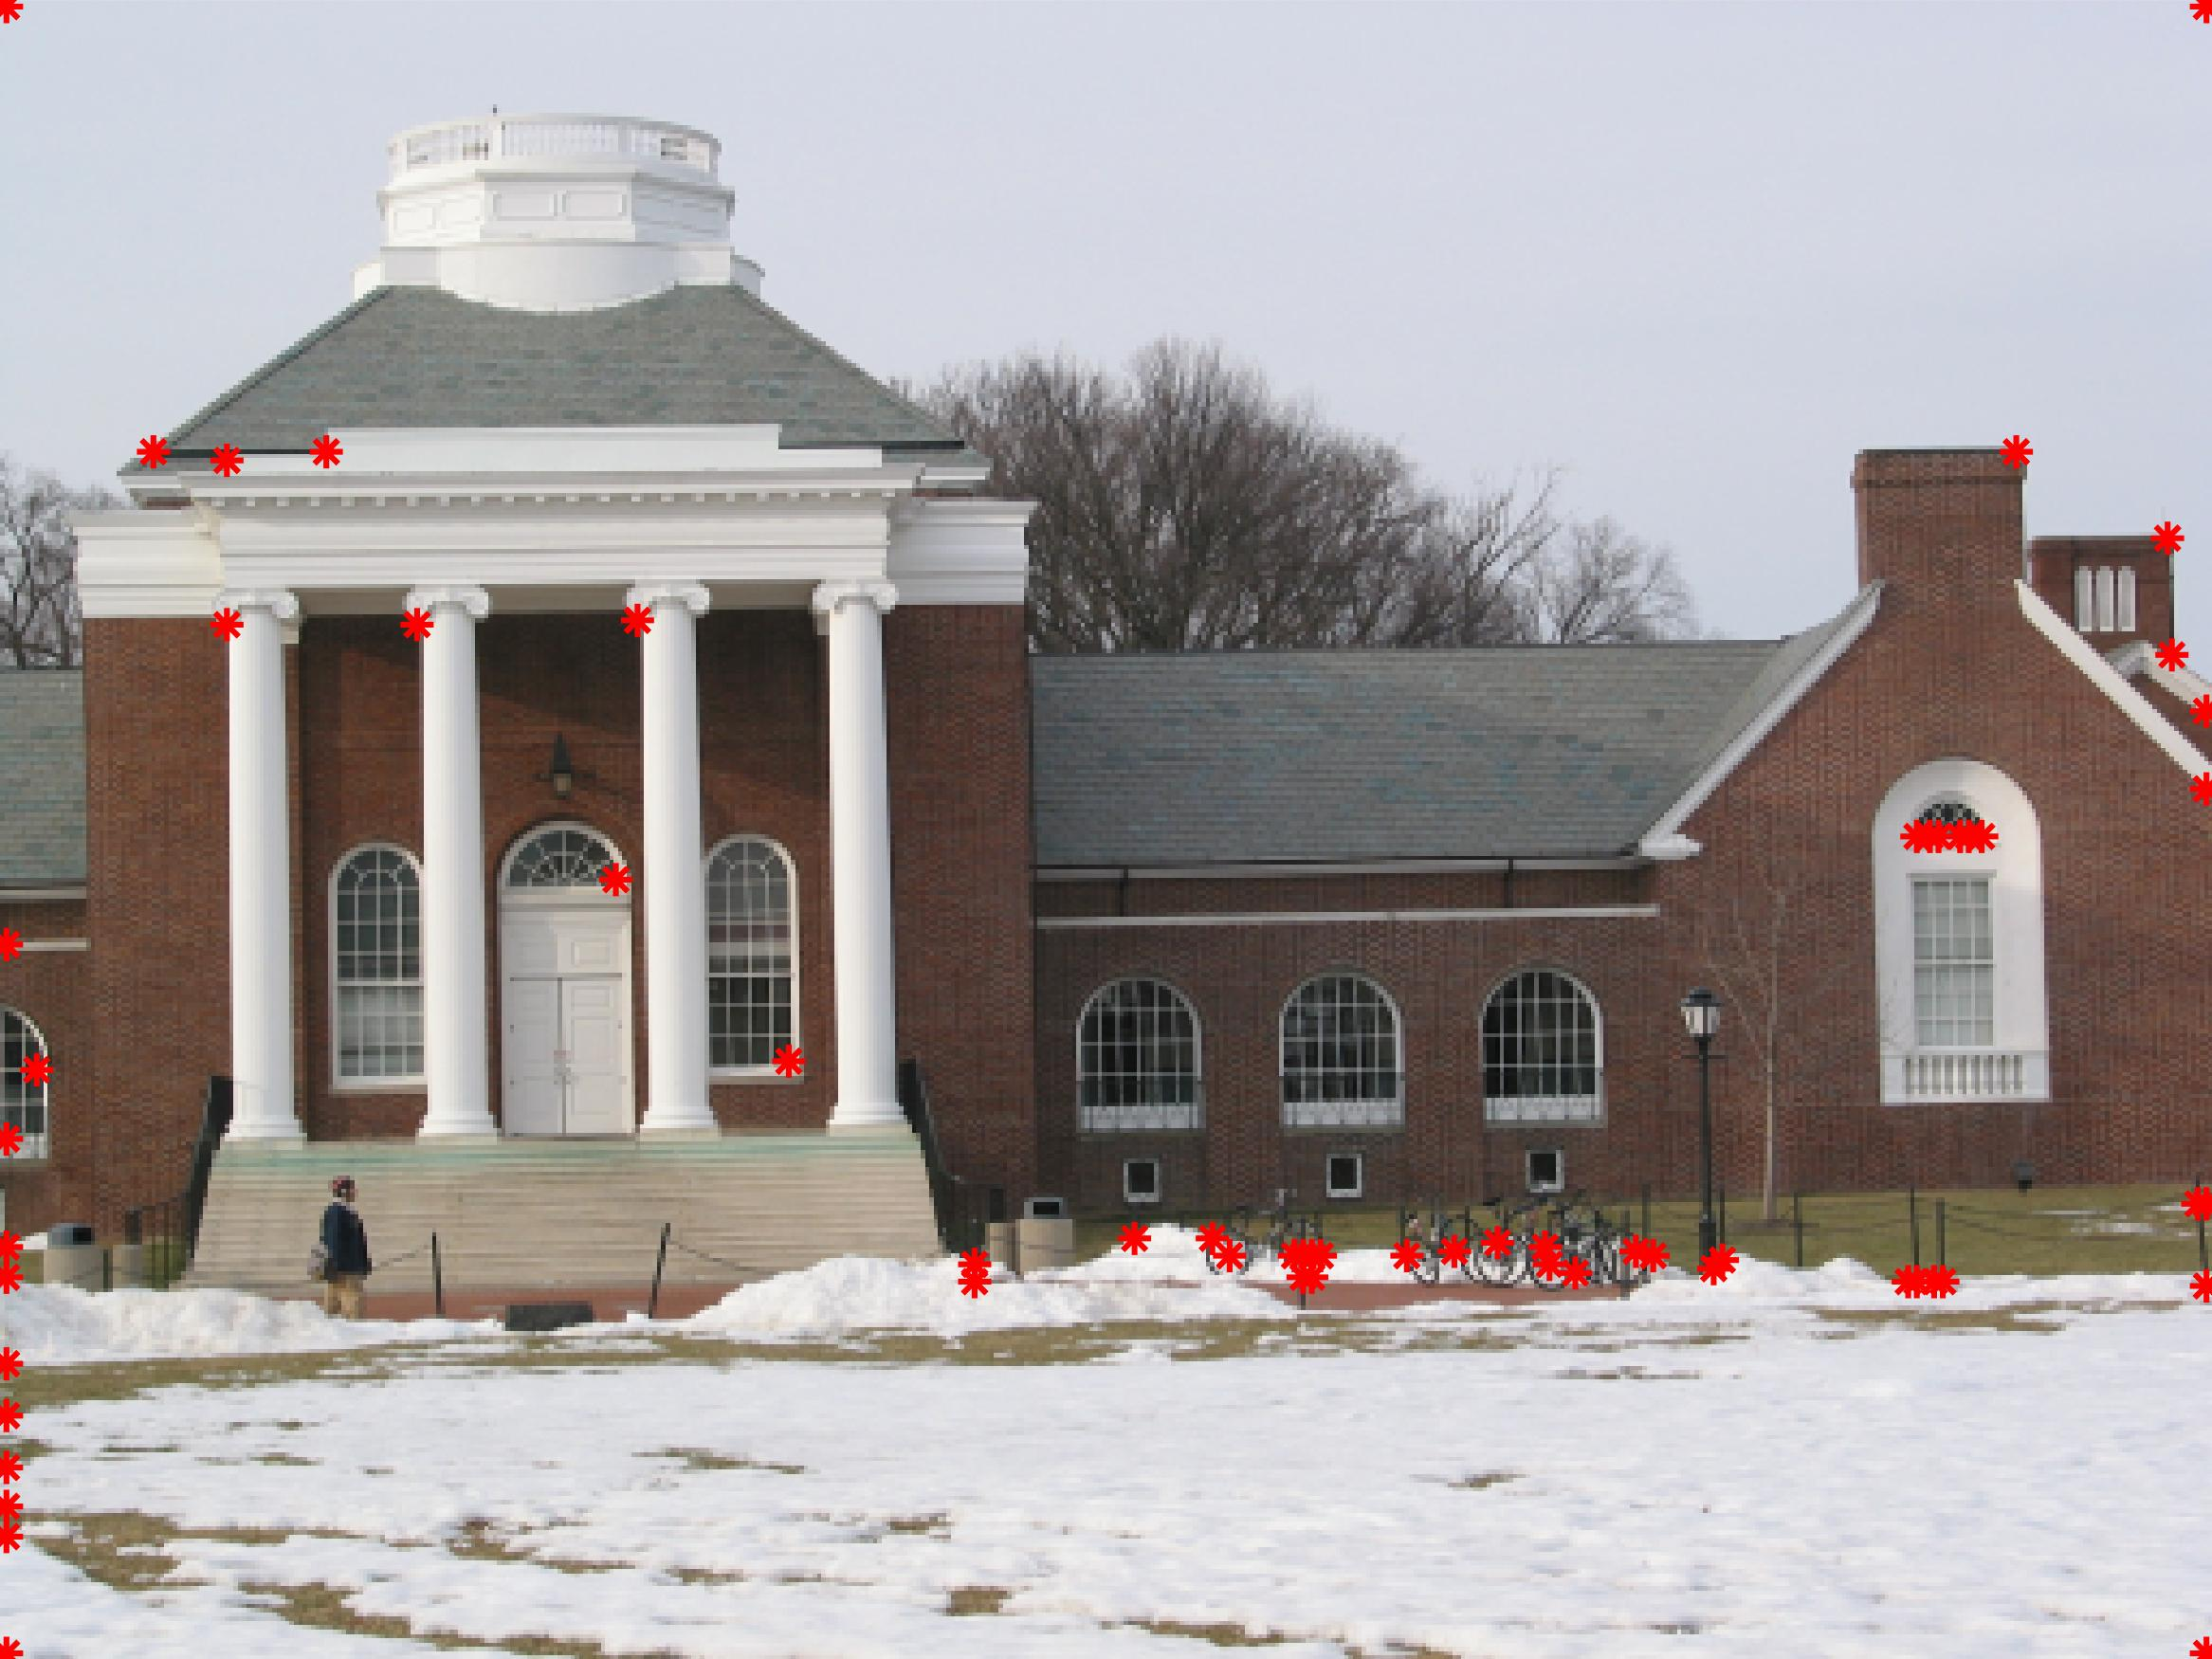
\includegraphics[width=0.45\columnwidth]{HW4_q1_c_t_1_I3.jpeg}
}
\caption{Harris Corner Detection results with different threshold, $T = tR_{max}, t=0.1$}
\label{q1_c_t_1}
\end{figure}

By comparing these Figures, we can see that a reasonable result is shown when $T = 0.01R_{max}$.\\

From Figure \ref{q1_c_t_001}, more edge points were detected than the actual corner points when $T = 0.001R{max}$ , indicating this threshold is too low. \\
Same reasoning, when $T = 0.1R_{max}$ and $T = 0.05R_{max}$, detection results tend to lose some corner points, indicating these thresholds are too high.\\

In conclusion, $t=0.01$ may be an ideal threshold for $T = t\cdot R_{max}$.\\
\clearpage


%%%%%%%%%%%%%%%%%%%%%%%%%%%%%%%%%%%%%%%%%%%%%%%%%%%%%%%%%%%%%%%%%%%%%%%%%%%%%%%
% Solution for Question 2 begins here - by Fan Bu
%%%%%%%%%%%%%%%%%%%%%%%%%%%%%%%%%%%%%%%%%%%%%%%%%%%%%%%%%%%%%%%%%%%%%%%%%%%%%%%
\section*{Question 2, Blob Detection}
\subsection*{(a)}
\subsubsection*{(1)}
Algorithm outline:\\
1. Build a Laplacian scale space, starting with some initial scale and going for $n$ iterations.\\
2. Generate a scale-normalized Laplacian of Gaussian filter at a given scale "$sigma$".\\
3. Filter image with the scale-normalized Laplacian. \\
4. Save square of Laplacian filter response for current level of scale space. \\
5. Determine threshold by multiply the scale with a factor $k$. \\
6. Perform non-maximum suppression in scale space. \\
7. Display resulting circles at their characteristic scales.\\

Codes are attached at the bottom of this question.\\
\subsubsection*{(2)}
The safety factor $k$ should depend on the largest scale at which we want regions to be detected. Therefore, the thresholds are chosen as $T = k\cdot scaleSpace_{max}$, where $scaleSpace_{max}$ is defined as the maximum scale space representation and takes value of $1.1669\times 10^4$. Take $k = 0.1, 0.2, 0.3, 0.4$, and results are shown in Figure \ref{HW4_q2_k_01},\ref{HW4_q2_k_02},\ref{HW4_q2_k_03},\ref{HW4_q2_k_04}. The exact threshold $T$ can be seen on the top of the figures.\\
\begin{figure}[H]
\begin{center}
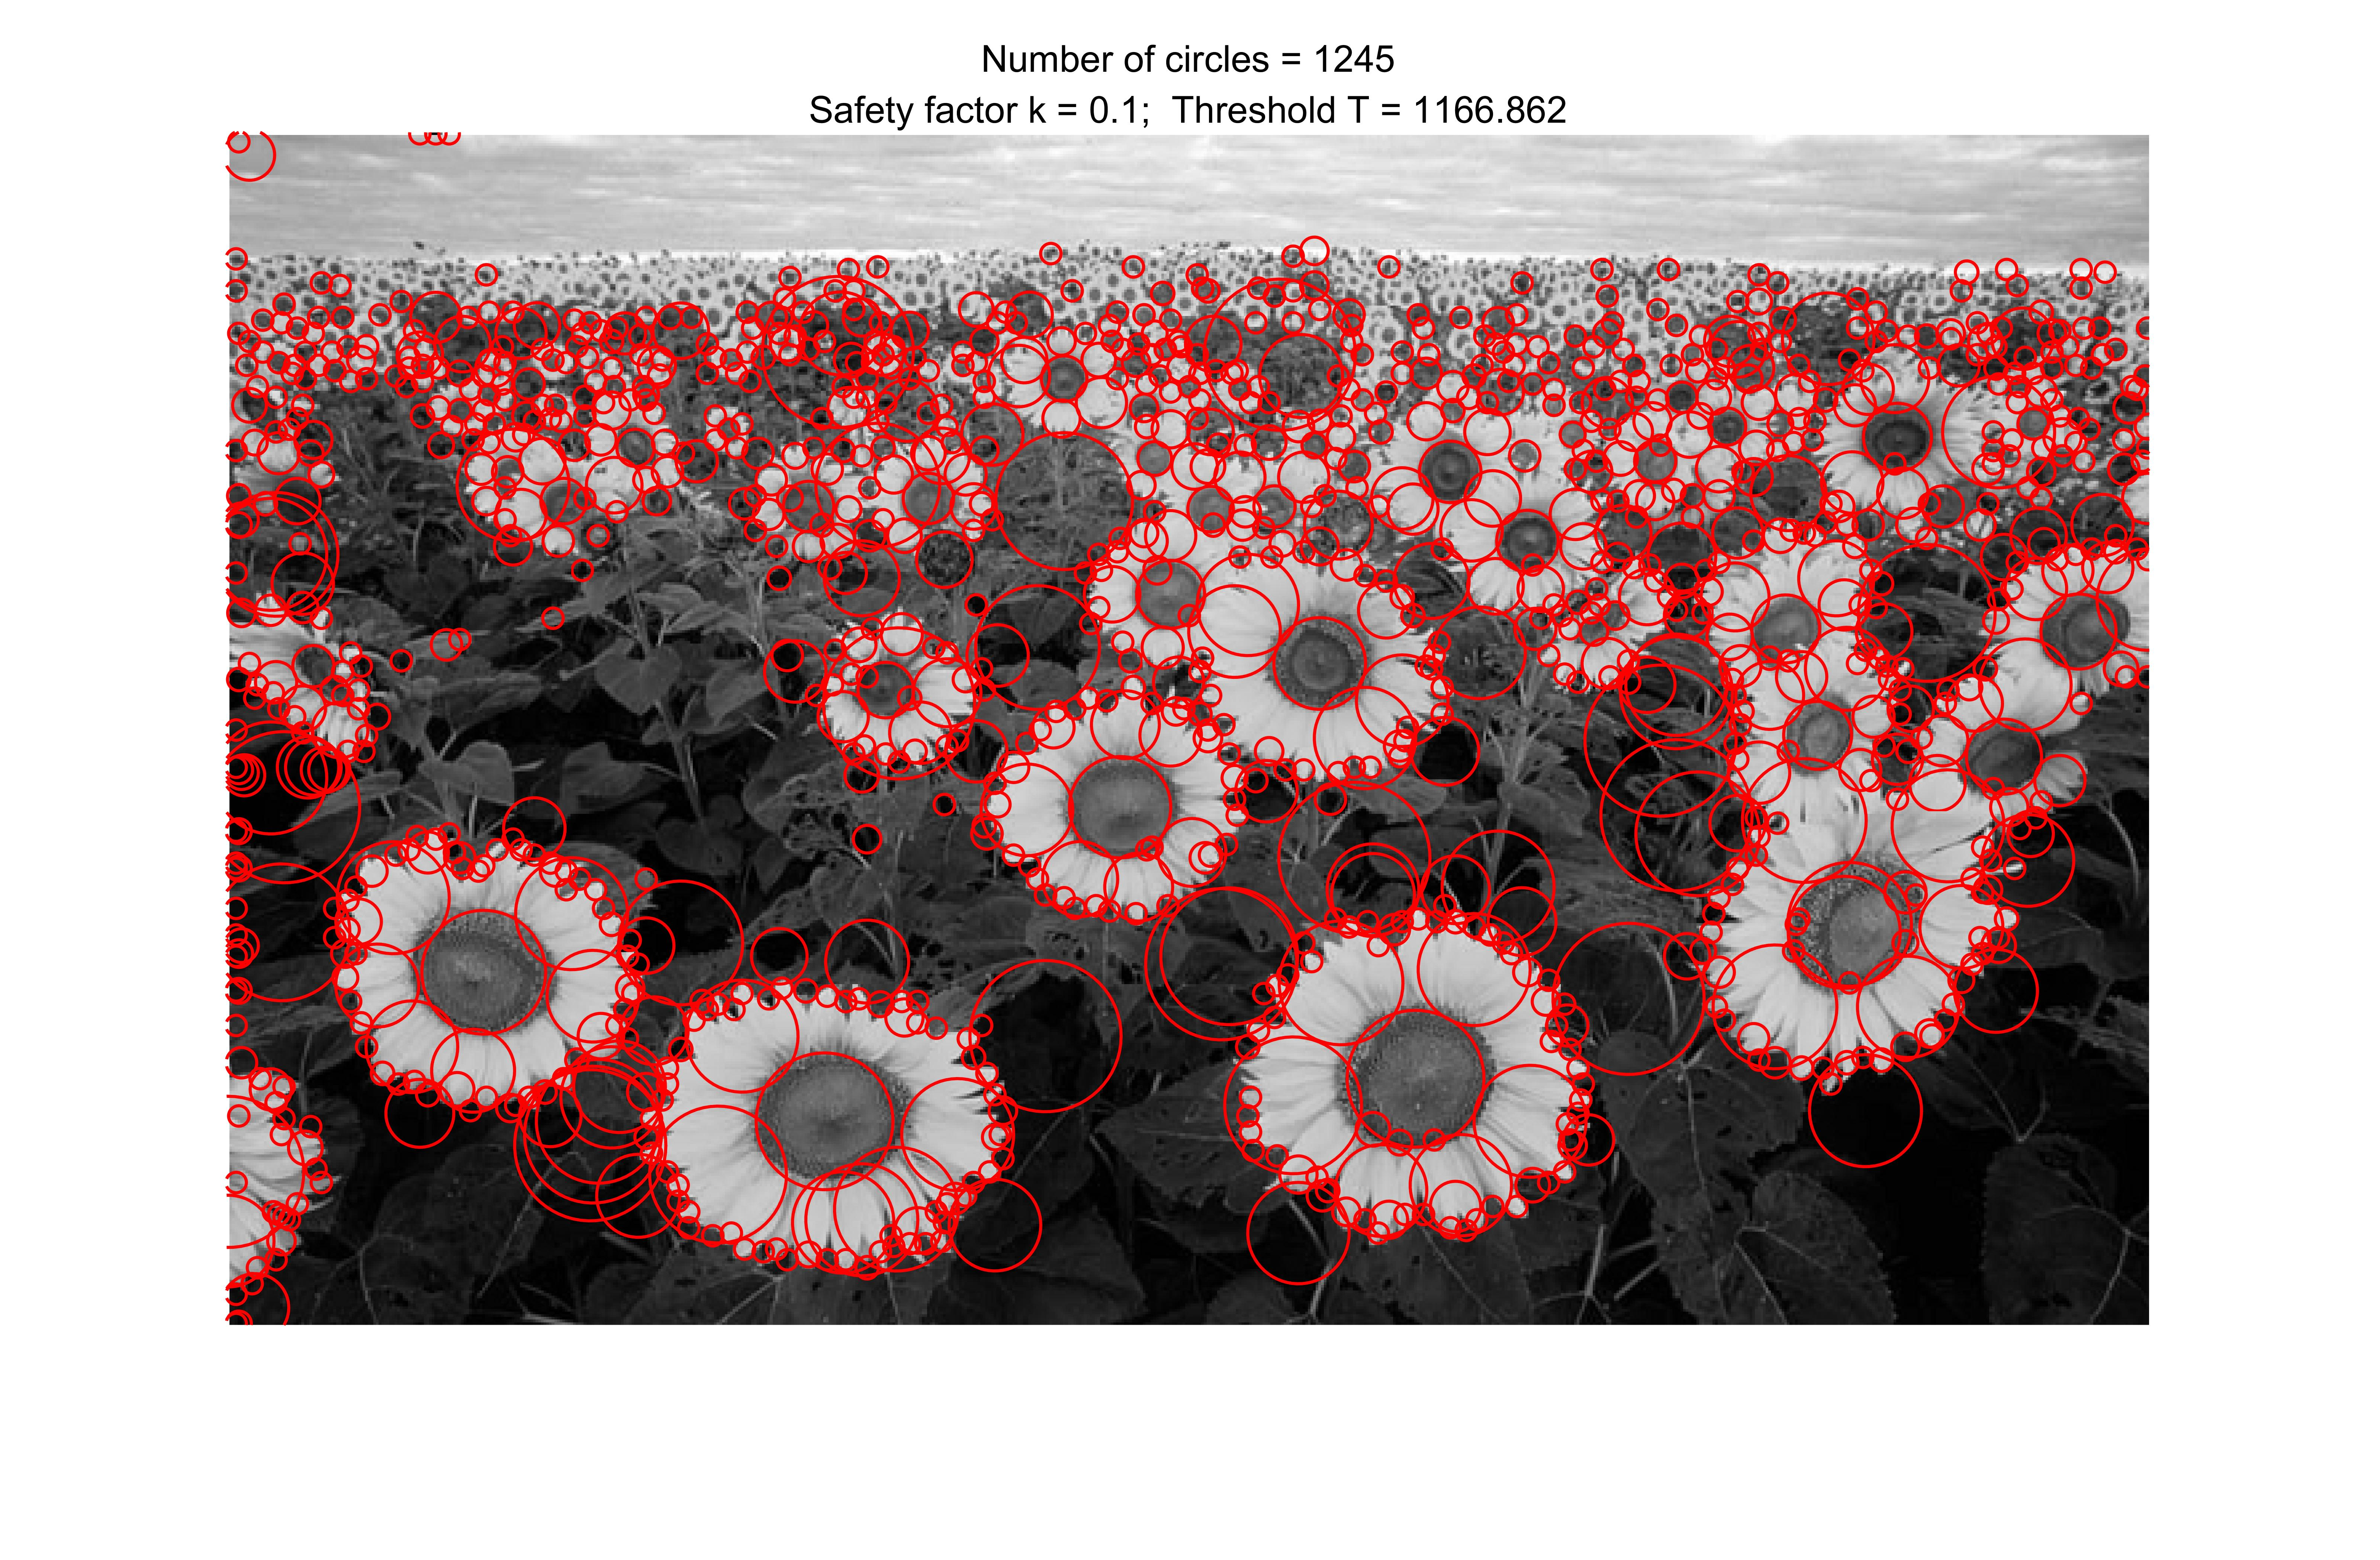
\includegraphics[width = 14cm]{HW4_q2_k_01.jpeg}
\end{center}
\caption{Harris Corner Detection results with $k=0.1$, $T\approx 1166$}
\label{HW4_q2_k_01}
\end{figure}

\begin{figure}[H]
\begin{center}
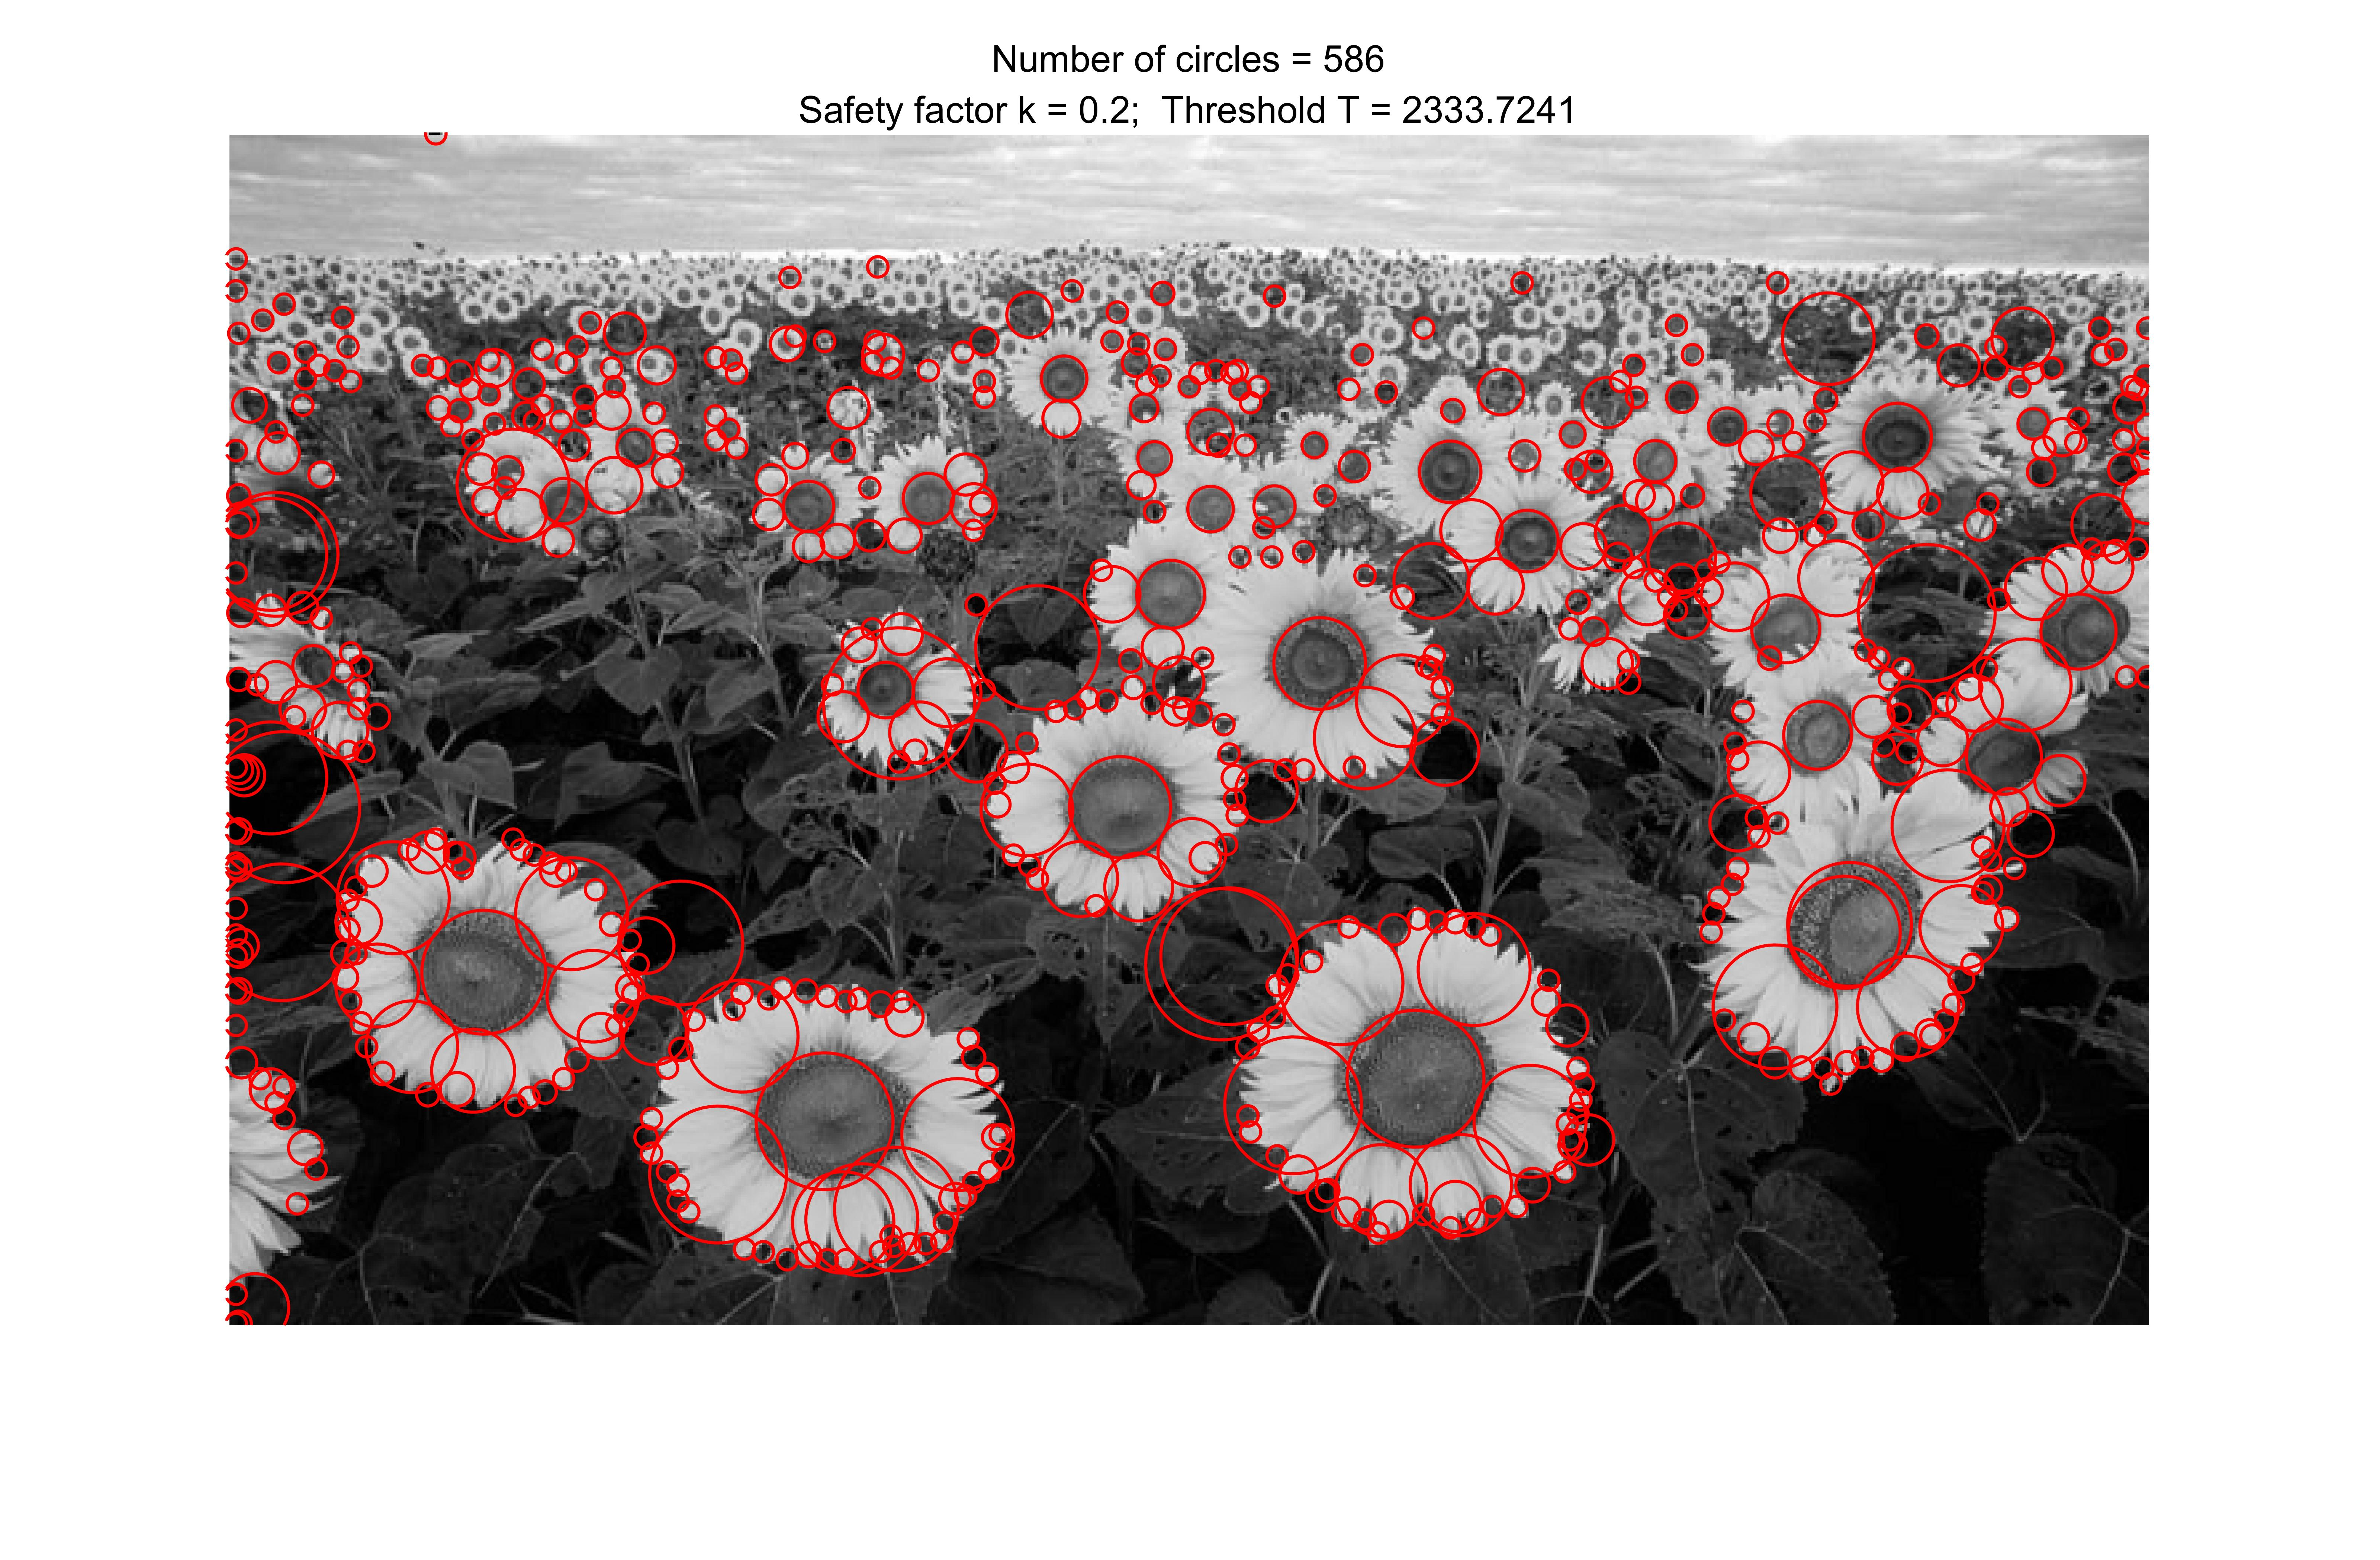
\includegraphics[width = 14cm]{HW4_q2_k_02.jpeg}
\end{center}
\caption{Harris Corner Detection results with $k=0.2$, $T\approx 2333$}
\label{HW4_q2_k_02}
\end{figure}

\begin{figure}[H]
\begin{center}
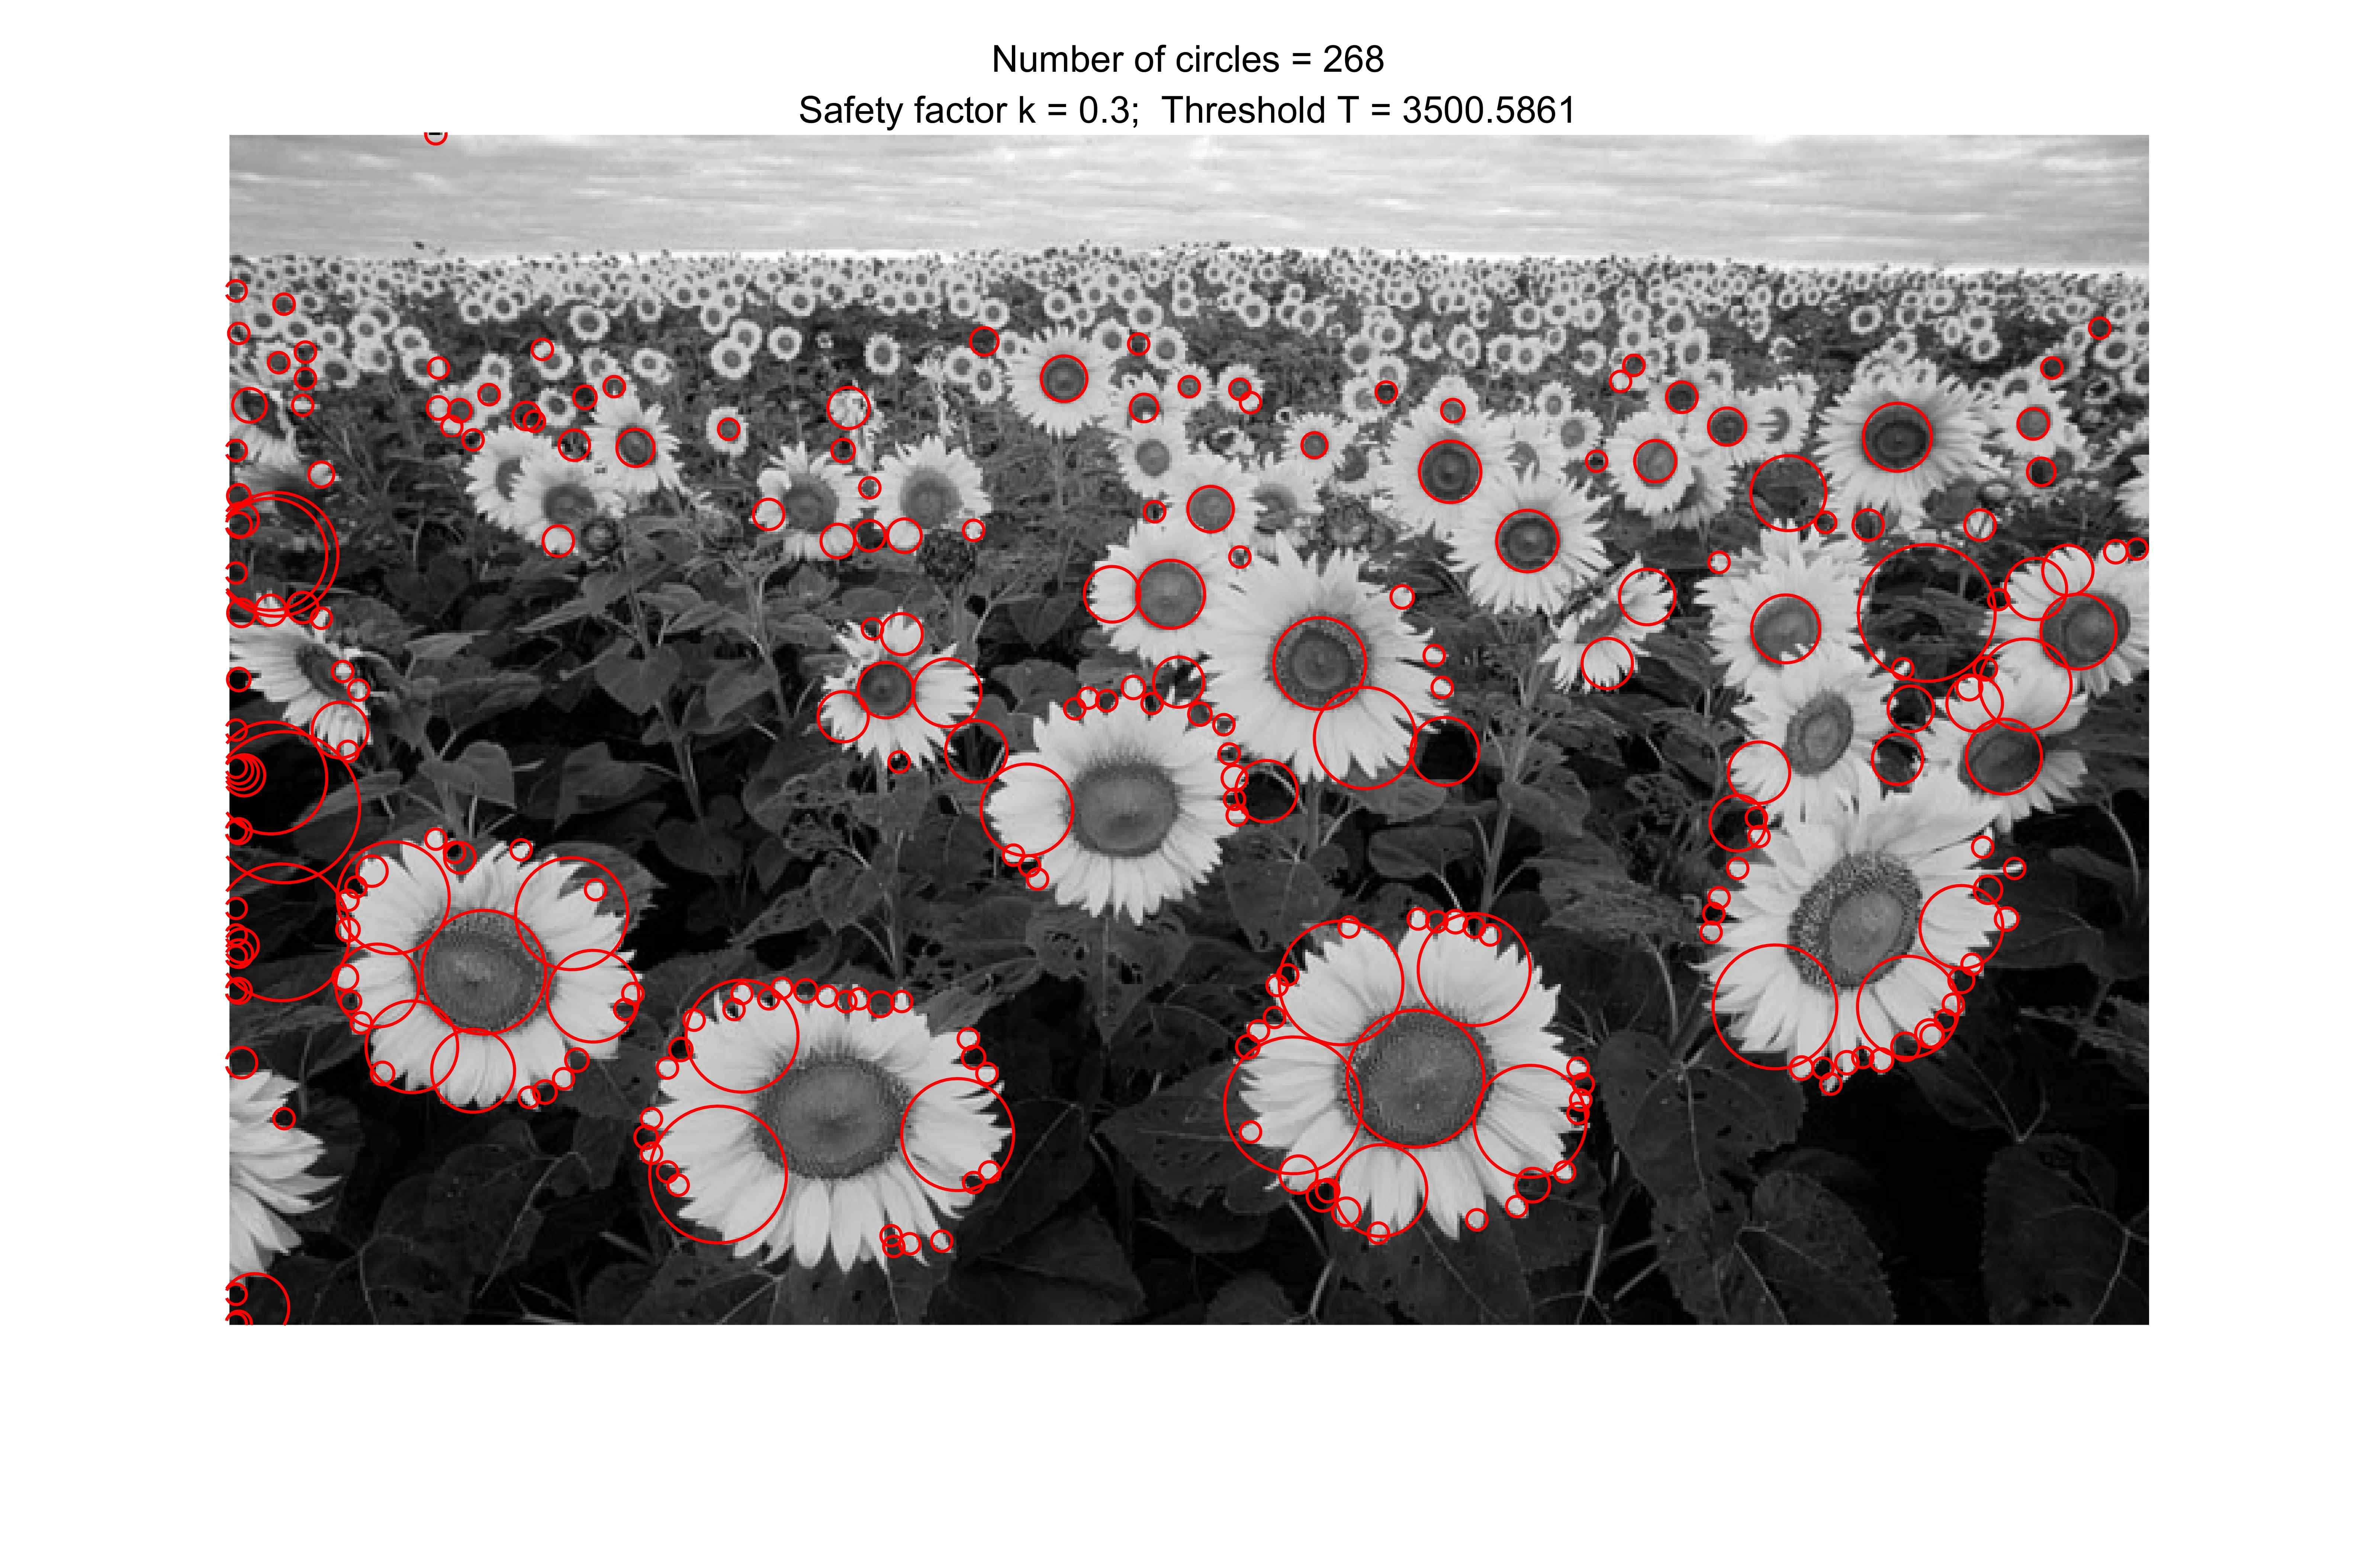
\includegraphics[width = 14cm]{HW4_q2_k_03.jpeg}
\end{center}
\caption{Harris Corner Detection results with $k=0.3$, $T\approx 3500$}
\label{HW4_q2_k_03}
\end{figure}

\begin{figure}[H]
\begin{center}
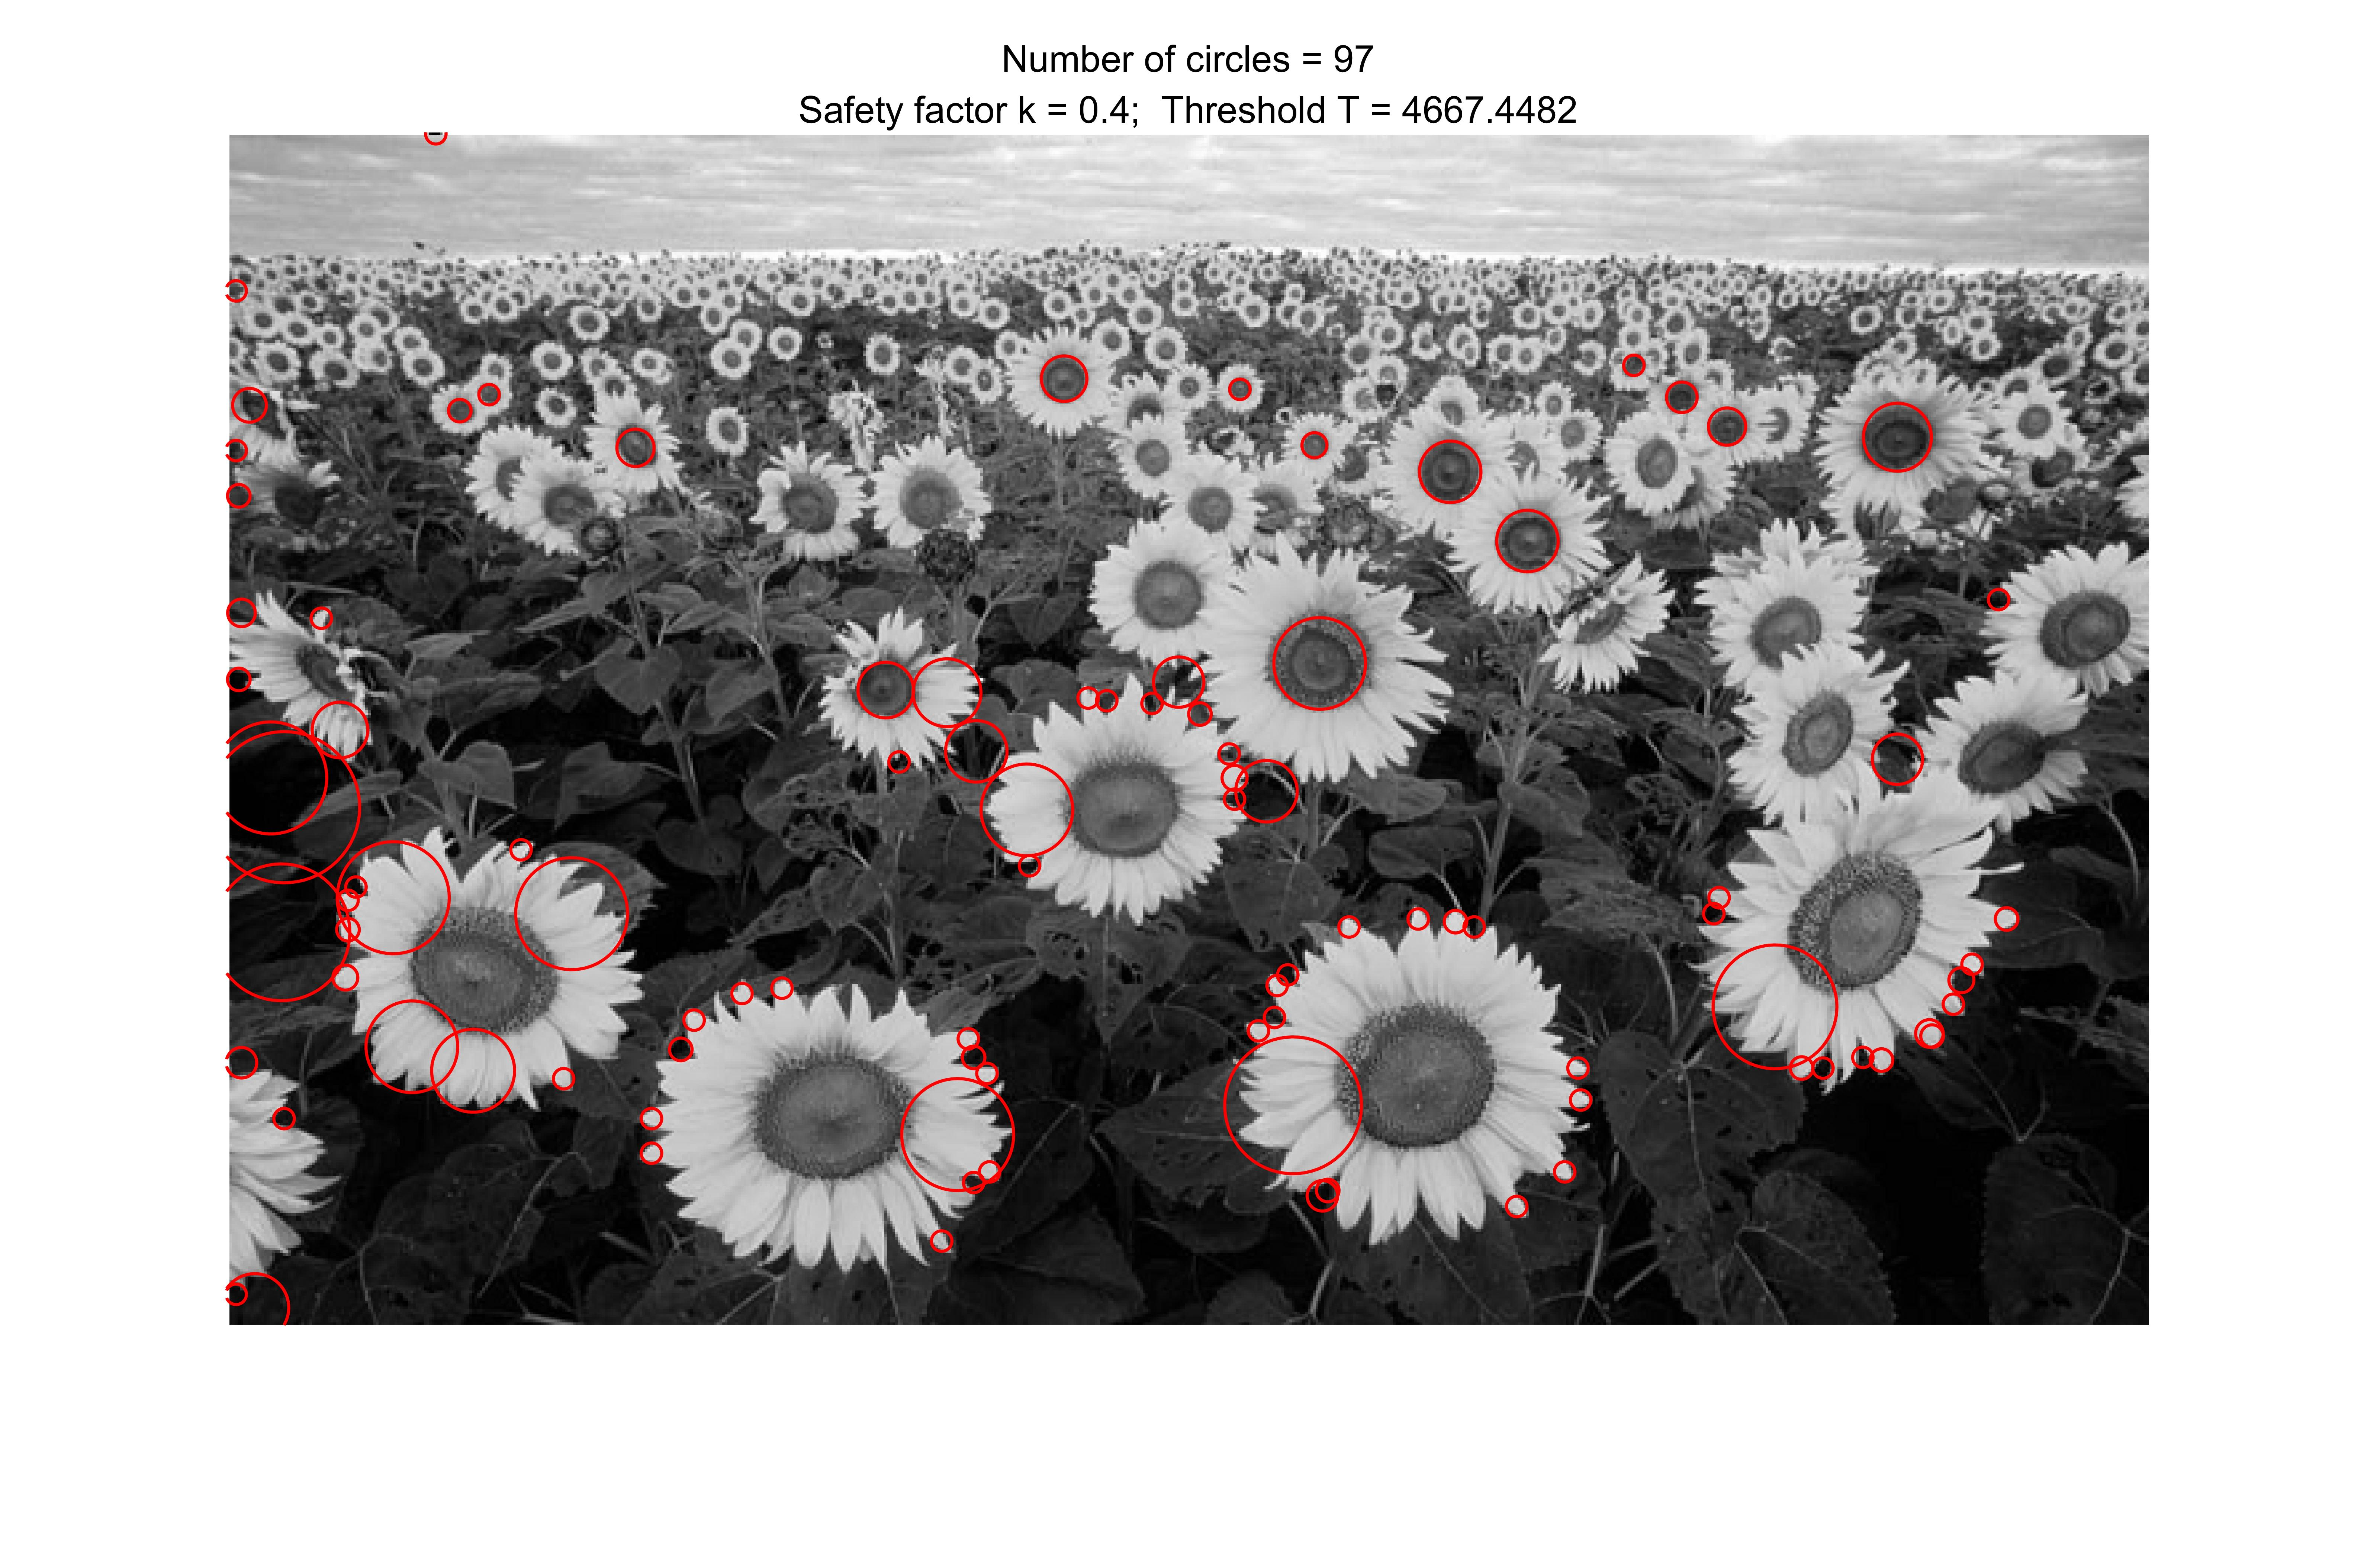
\includegraphics[width = 14cm]{HW4_q2_k_04.jpeg}
\end{center}
\caption{Harris Corner Detection results with $k=0.4$, $T\approx 4667$}
\label{HW4_q2_k_04}
\end{figure}

From the figures above, we can see that while $k = 0.2$ captures a reasonable result. When $k = 0.3$, less blobs are detected but still acceptable. \\
While $k = 0.1$ includes some dummy points in the picture, for example those blobs in the sky, indicating this threshold is too small. Same reasoning, when $k = 0.4$, the detection only capture very limited nearby blobs. In that case, the threshold is too high. \\

\subsection*{(b)}
The detection result of $T = 1500$ is shown below in Figure \ref{HW4_q2_c_k_012855}:\\
\begin{figure}[H]
\begin{center}
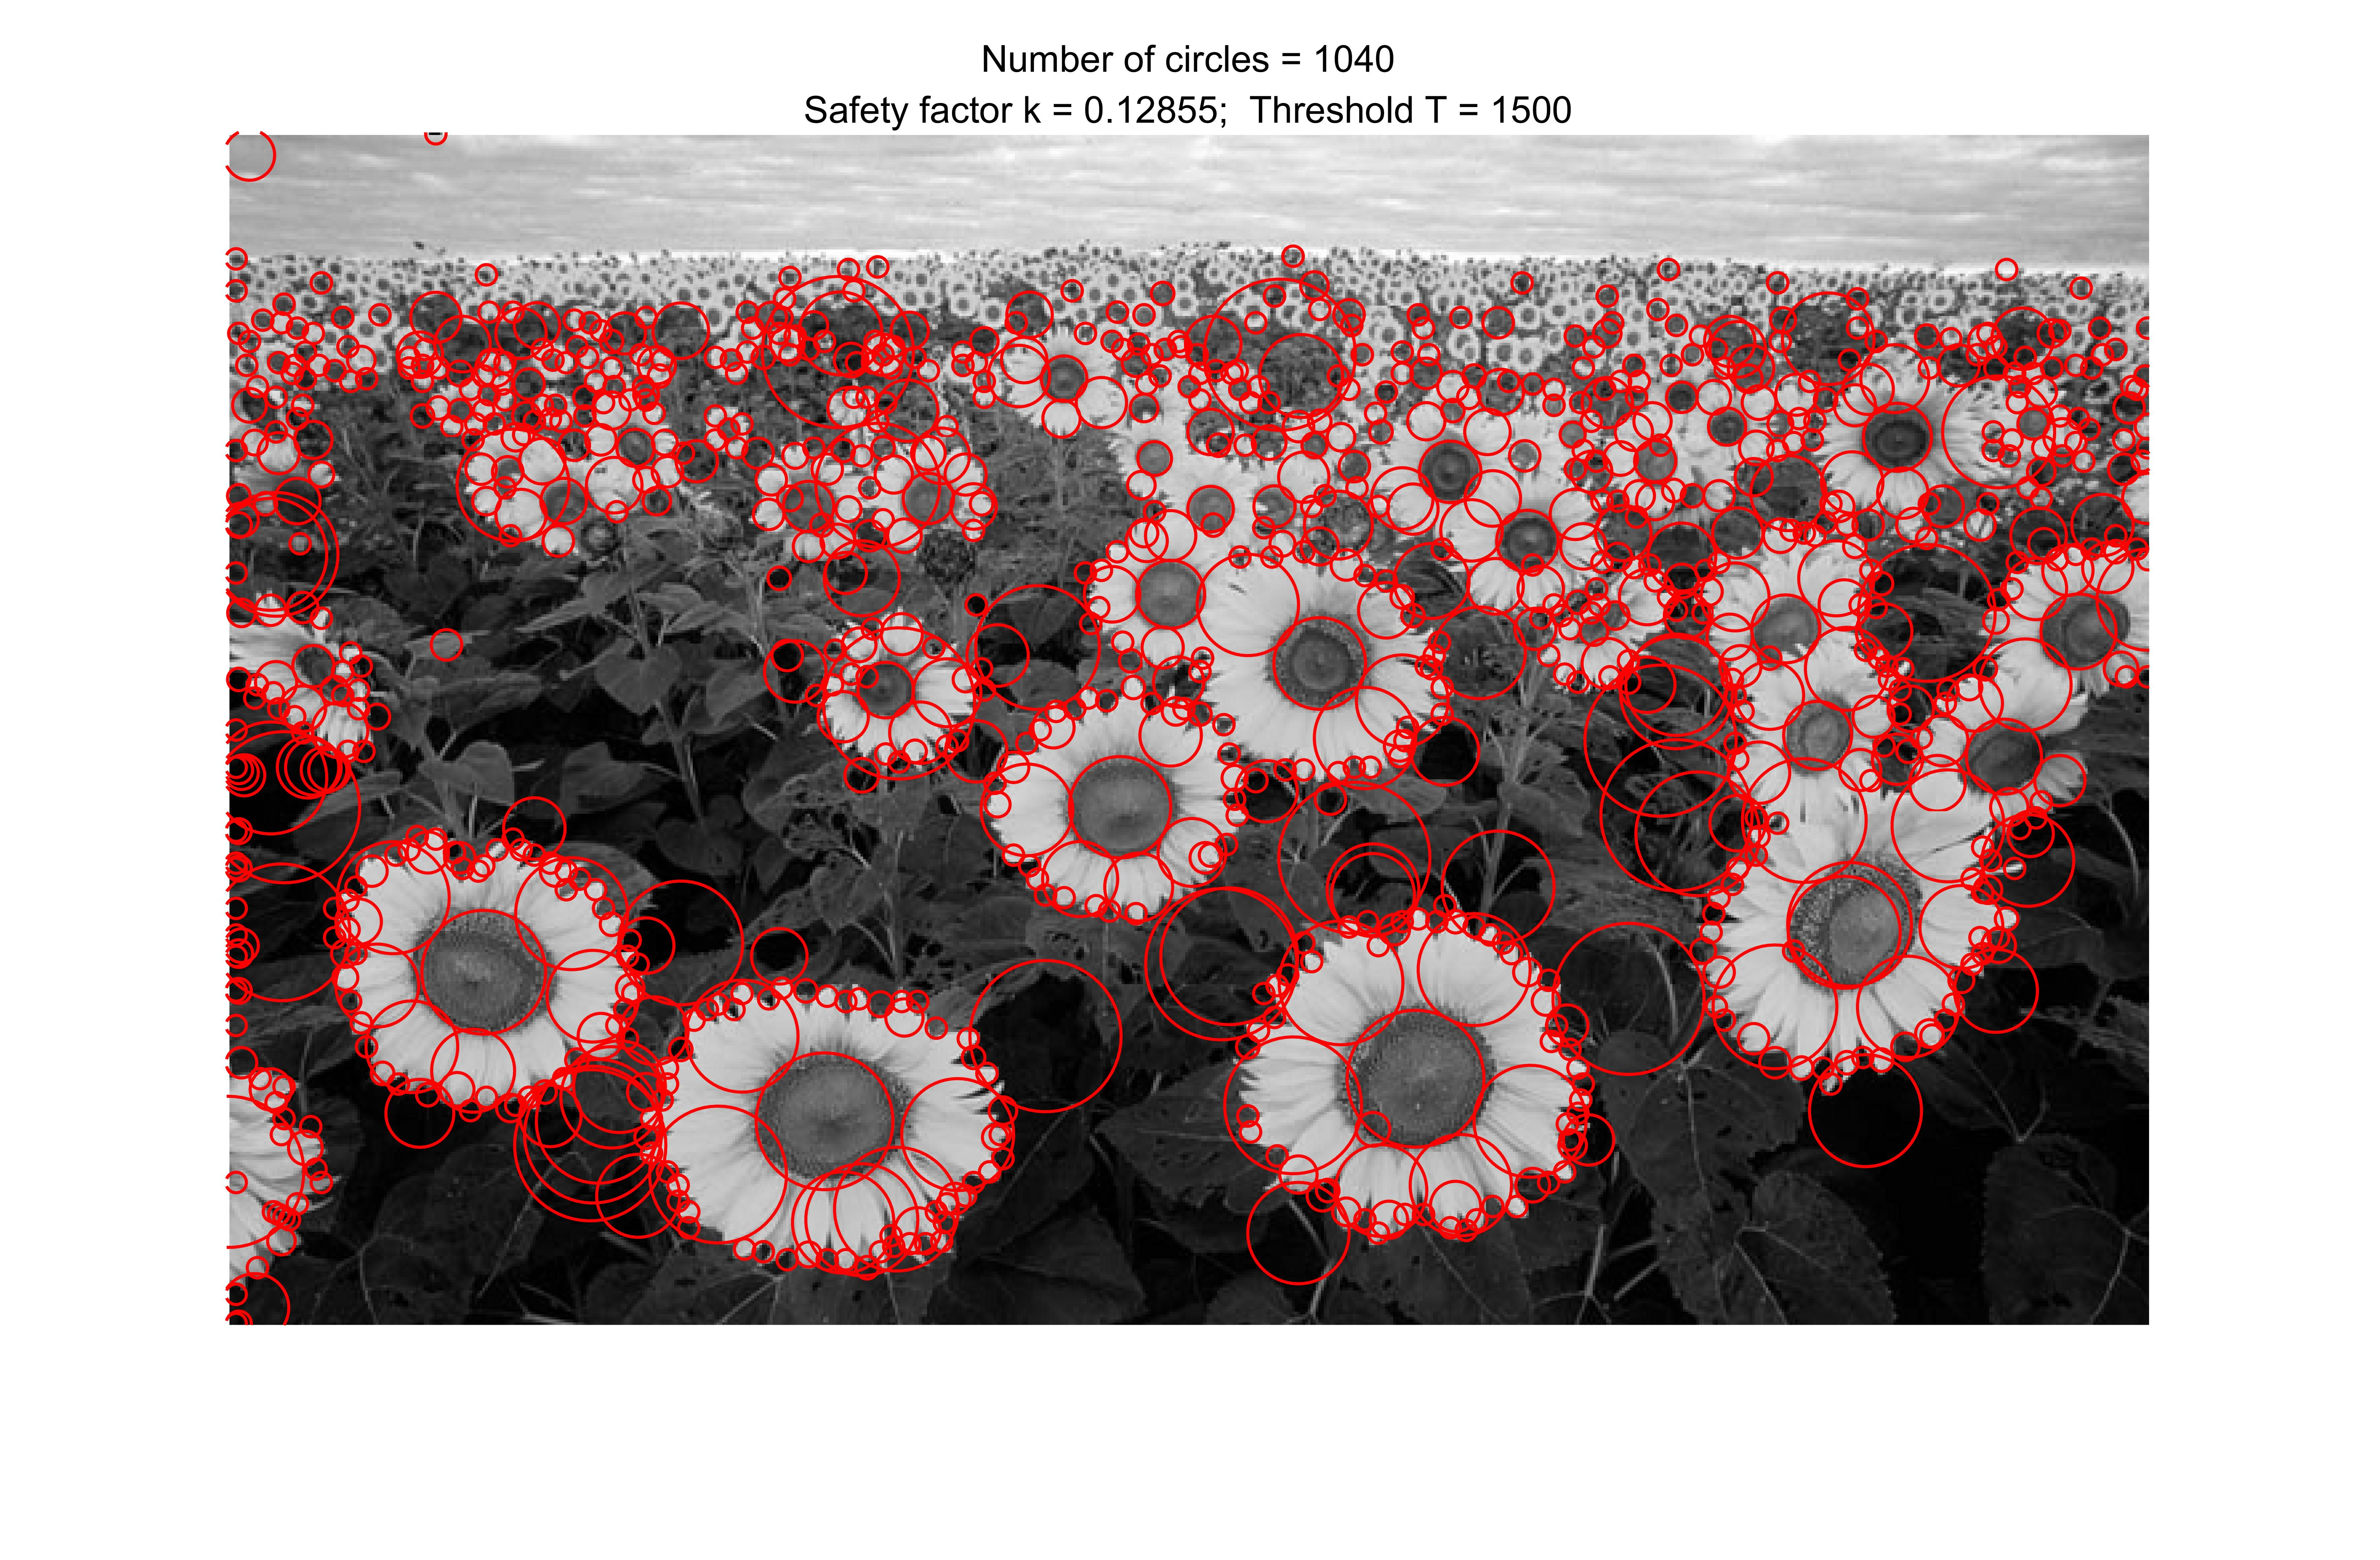
\includegraphics[width = 12cm]{HW4_q2_c_k_012855.jpeg}
\end{center}
\caption{Harris Corner Detection results with $k=0.12855$, $T = 1500$}
\label{HW4_q2_c_k_012855}
\end{figure}

The histogram of normalized radii is shown in Figure \ref{HW4_q2_c_hist}, and maximum radius is also shown on the title.\\
\begin{figure}[H]
\begin{center}
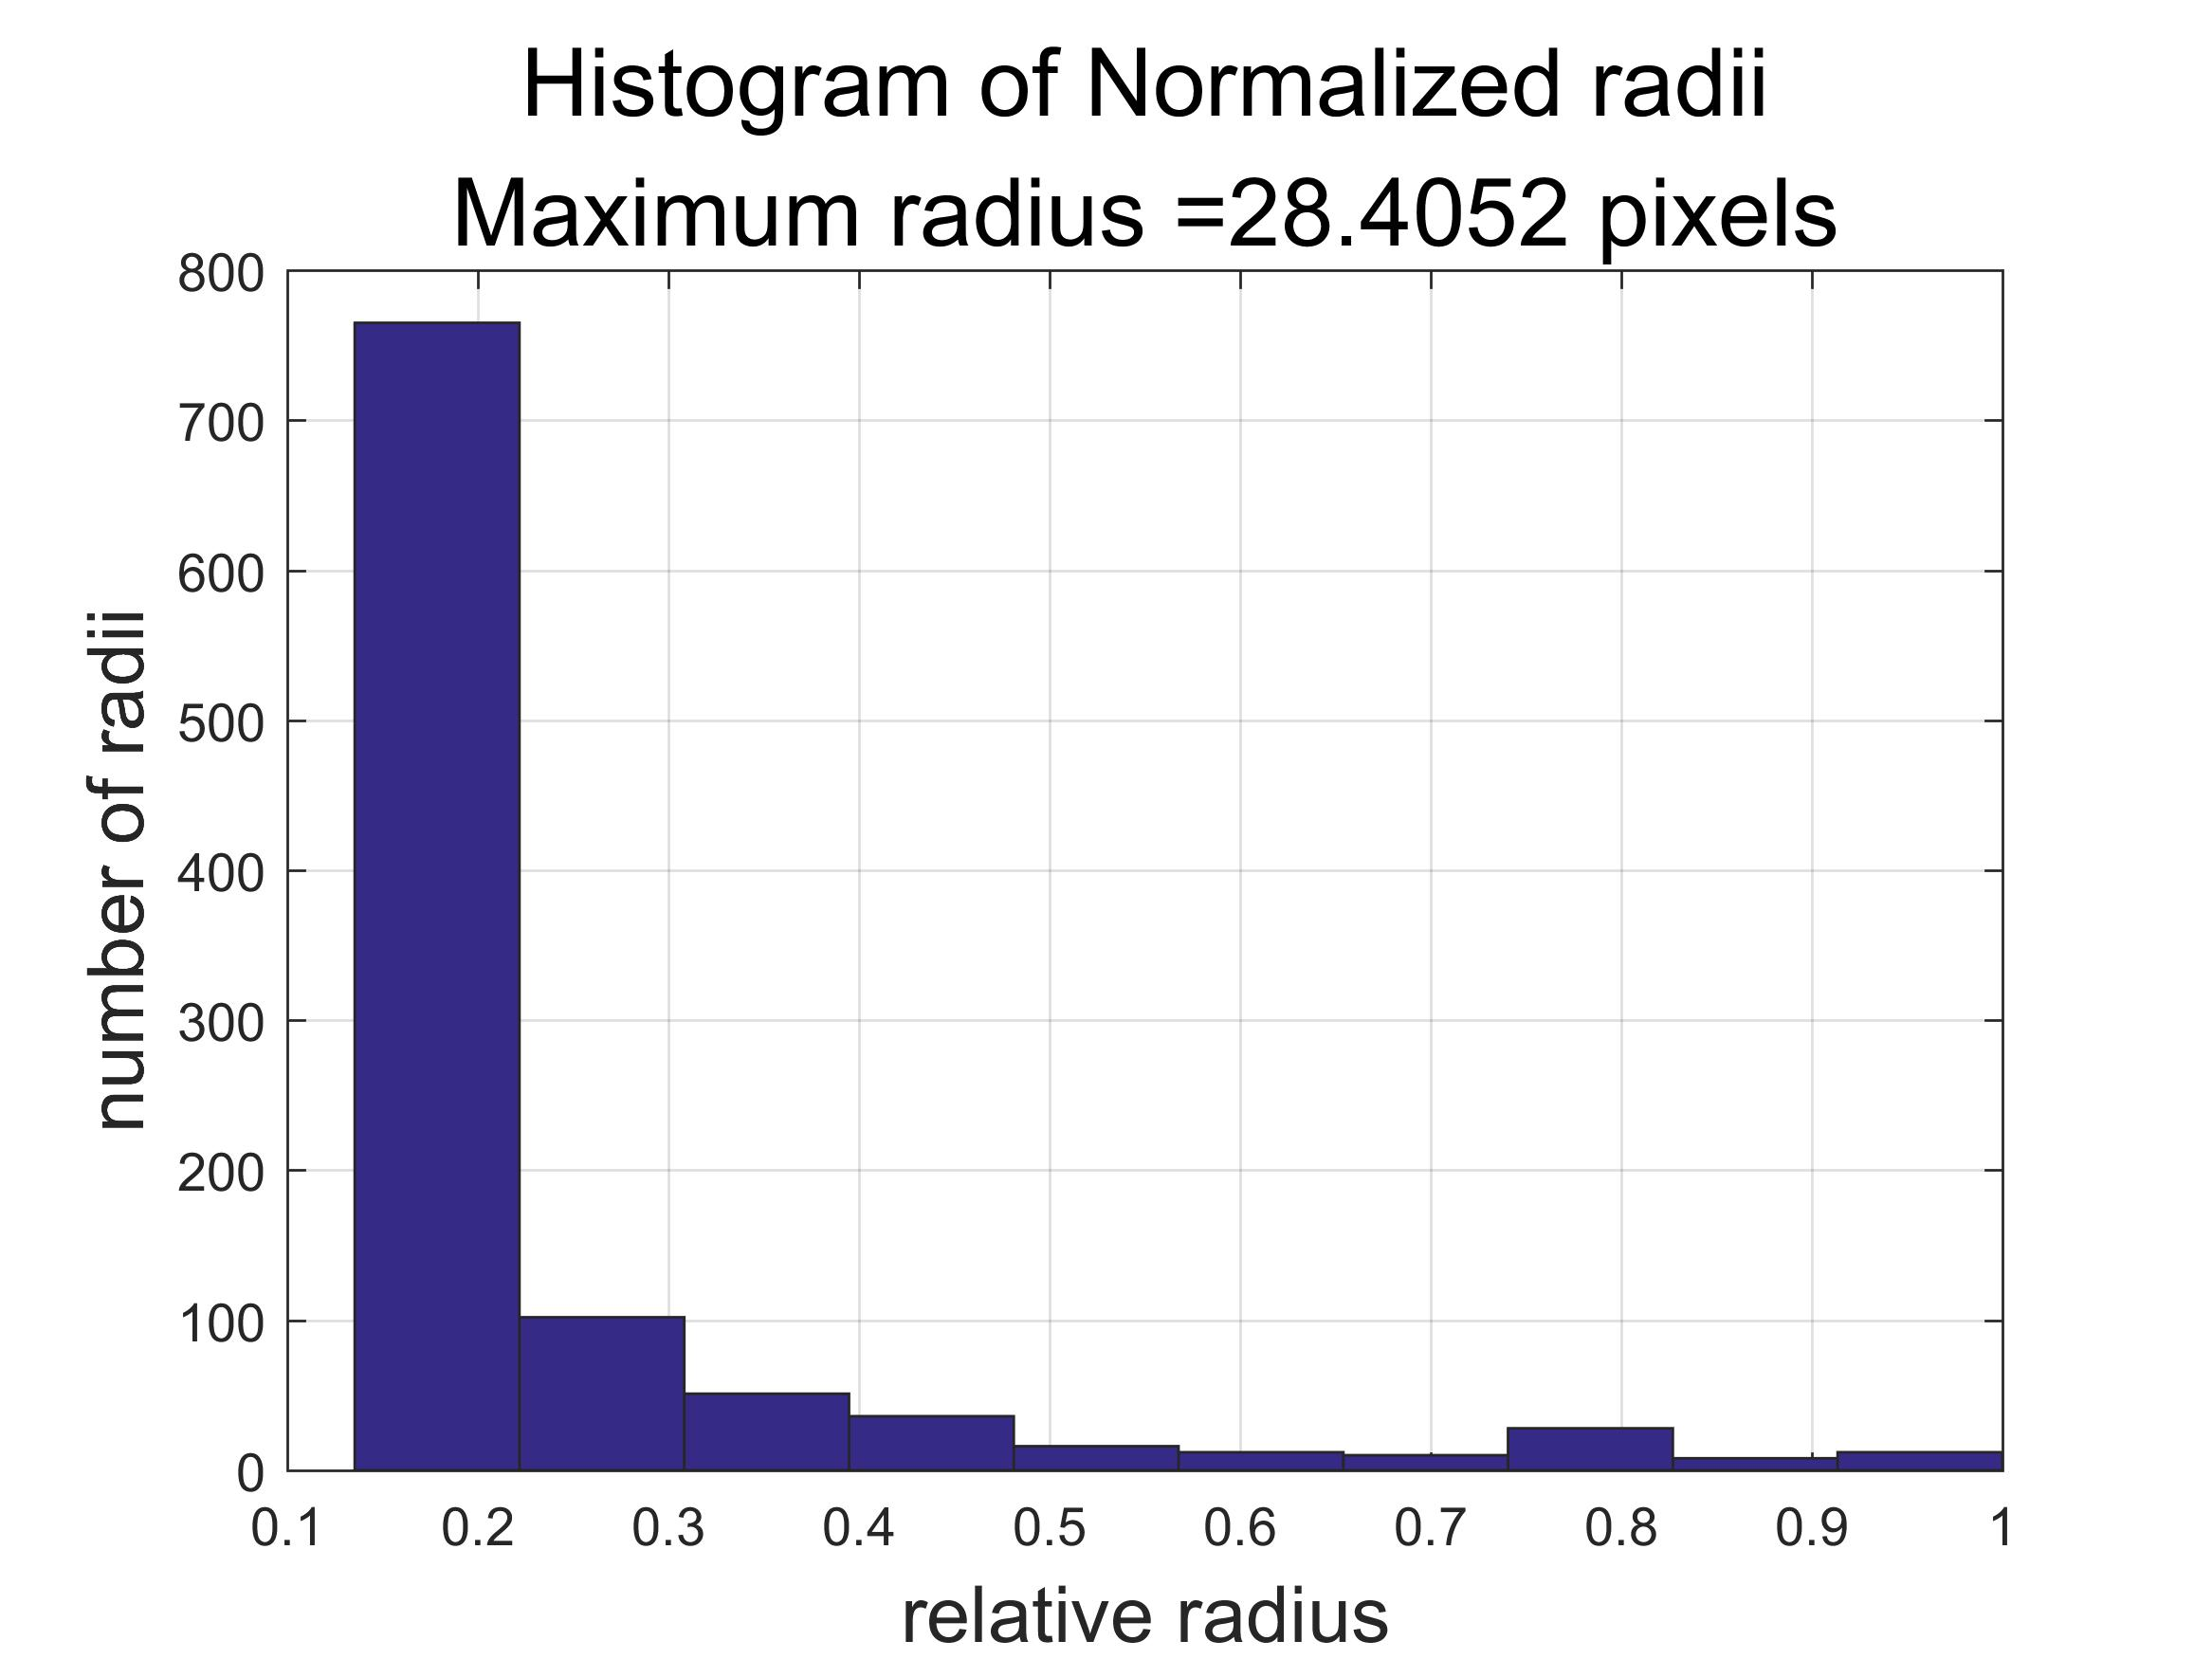
\includegraphics[width = 12cm]{HW4_q2_c_hist.jpeg}
\end{center}
\caption{Histogram of Normalized radii with $T = 1500$, $bin = 10$}
\label{HW4_q2_c_hist}
\end{figure}

\subsection*{Matlab Codes}
\begin{lstlisting}
%% EECS 442 - HW 04 - Q2 Blob Detection
%  ------------------------------------------------------------------------
%  Date: 11 / 21 / 2016
%  Author: Fan Bu
%  ------------------------------------------------------------------------
%  show_all_circles(I, cx, cy, rad, color, ln_wid)
%  ------------------------------------------------------------------------
%  Instructions:
%  Implement a blob detector based on the Laplacian operator and
%  characteristic scale concept introduced by Lindeberg. Compute the radius
%  of each blob (in pixels) and report the histogram (dis- tribution)
%  of radii computed for the whole image.
%
% Algorithm outline:\\
% 1. Build a Laplacian scale space, starting with some initial scale and going for $n$ iterations.\\
% 2. Generate a scale-normalized Laplacian of Gaussian filter at a given scale "$sigma$".\\
% 3. Filter image with the scale-normalized Laplacian. \\
% 4. Save square of Laplacian filter response for current level of scale space. \\
% 5. Determine threshold by multiply the scale with a factor $k$. \\
% 6. Perform non-maximum suppression in scale space. \\
% 7. Display resulting circles at their characteristic scales.\\

%% Initialization
clear all;
close all;
clc;
%% ------------------- Parameter selection -----------------------
t = 1:0.1:3;
sigma = exp(t);
sigma = sigma';
levels = length(sigma);
%% ------------------- Load data --------------------------------
img = imread('3.bmp');
img = rgb2gray(img);
double_img = double(img);

% Build a Laplacian scale space, starting with some initial scale and going for $n$ iterations.
[height width] = size(img);
scale_space = zeros(height,width,levels);

%% ------------------- Perform detection ------------------------

for i=1:levels

% Generate a scale-normalized Laplacian of Gaussian filter at a given scale "$sigma$".
filter_size = 2*ceil(3*sigma(i))+1;
kernel = fspecial('log', filter_size, sigma(i));
% Filter image with the scale-normalized Laplacian.
nLoG = sigma(i)^2 * kernel;
Filtered_img = imfilter(double_img, nLoG, 'same', 'replicate');
Filtered_img = Filtered_img .^ 2;
% Save square of Laplacian filter response for current level of scale space.
scale_space(:,:,i) = Filtered_img;
end
% choose the right thresold T, as T = k * scaleSpace_{max}.
k = 0.4;
max_scale_space = max(max(max(scale_space)))
T = k * max_scale_space
% choose the right thresold T =1500 for this question.
T = 1500
k = T/max_scale_space
% Perform non-maximum suppression in the 3D scale space
scale_space_filtered = zeros(height,width,levels);
for i=1:levels
    scale_space_filtered(:,:,i) = ordfilt2(scale_space(:,:,i),9,ones(3));
end
for i = 1:levels
    scale_space_filtered(:,:,i) =  max(scale_space_filtered(:,:,max(i-1,1):min(i+1,levels)),[],3);
end
scale_space_filtered  = scale_space_filtered .* (scale_space_filtered == scale_space);

% calculate perameters for show_all_circles
row = [];
col = [];
radius = [];
for i=1:levels
    [new_rows,new_cols] = find(scale_space_filtered(:,:,i)>=T);
    num = length(new_rows);
    radii = sigma(i)*sqrt(2);
    radii = repmat(radii,num,1);
    row = [row;new_rows];
    col = [col;new_cols];
    radius = [radius;radii];
end
show_all_circles(img,col,row,radius);
set(gcf,'units','normalized','position',[0,0,0.8,1]);
h_title=title({['Number of circles = ', num2str(size(col,1))]
    ['Safety factor k = ',num2str(k), ';  Threshold T = ',num2str(T)]});
set(h_title,'FontSize',18);
print(gcf,'-djpeg' ,['HW4_q2_c_k_',num2str(k),'.jpeg'],'-r400')

% recompute 3d-indices of maxima
s = [height width levels];
%%  ------------------- draw blobs on image  ---------------------
figure
max_rad = max(radius);
radius = radius / max_rad;
hist(radius,10);
h_title=title({['Histogram of Normalized radii']
    ['Maximum radius =', num2str(max_rad),' pixels']});
set(h_title,'FontSize',18);
grid on
xlabel('relative radius','FontSize',15)
ylabel('number of radii','FontSize',15)
print(gcf,'-djpeg' ,['HW4_q2_c_hist.jpeg'],'-r400')
\end{lstlisting}
\end{document}
